\documentclass[letterpaper,12pt]{article}
%\documentclass[draft,twoside,letterpaper,12pt]{article}

\title{The Physics of God and the Quantum Gravity Theory of Everything\footnote{Originally published at the Social Science Research Network (SSRN) on December 19, 2011, doi:\discretionary{}{}{}\href{http://dx.doi.org/10.2139/ssrn.1974708}{10.2139/\dsc ssrn.1974708}\thinspace. Herein revised on \today . This article and its contents are released in the public domain. If one desires a copyright for this work, then this article and its contents are also released under Version 3.0 of the ``Attribution (By)'' Creative Commons license and\slash or Version 1.3 of the \textsc{Gnu} Free Documentation License. Note that this article incorporates various priorly-published writings of mine in diverse locations.}}

\author{James Redford\footnote{Email address: \textless\href{mailto:jrredford@yahoo.com}{jrredford@yahoo.com}\textgreater .}}

%\date{July 26, 2010} %\today

\usepackage[OT2,T1]{fontenc}
\usepackage{scalefnt}
\usepackage{afterpage}
\usepackage[absolute]{textpos}% showboxes
\usepackage[ibycus,english]{babel}
\usepackage{cjhebrew}
\usepackage[format=plain,small,bf]{caption}
\usepackage{subfig}
\usepackage{graphicx}
\usepackage{amsmath}
\usepackage[runin]{abstract}
\usepackage{thinsp}
\usepackage[charter]{mathdesign}
\usepackage{helvet}
\usepackage[hyphens,obeyspaces,spaces]{url}
\usepackage{epigraph}
\usepackage{geometry}
\usepackage{appendix}
\usepackage[noadjust,space]{cite}
%\usepackage[numbers,sort&compress]{natbib}
\usepackage[backref=page]{hyperref}% hyperref options: hyperindex, backref=page, breaklinks
\usepackage[sanitize={symbol=false},acronym,section,toc]{glossaries}% nonumberlist
\usepackage{tikz}
\usepackage{calc}
\usepackage{attachfile}
%\usepackage[hyphenbreaks]{breakurl}

% used by textpos
\setlength{\TPHorizModule}{1in}
\setlength{\TPVertModule}{1in}

\newlength{\Urlname}
\newcommand{\doubleprint}[1]{\setlength{\Urlname}{\widthof{#1}}}
\newcommand{\textattachfileandprintout}[2]{%
\textattachfile[color=0 0 1]{#1}{#2}\doubleprint{#2}\hspace{-\Urlname}#2}

\newcounter{HawkingEnergyZ}

\newcounter{UniverseAccelerationZ}

\newcounter{AnimalSacrificesZ}

\urlstyle{sf}
%\urlstyle{rm}
%\urlstyle{same}

%\noindent

\abslabeldelim{\mbox{:\hspace{-0.25em}\quad}}

\newcommand\textcyr[1]{{\fontencoding{OT2}\fontfamily{wncyr}\selectfont #1}}

\setlength{\epigraphwidth}{3.67in}

\renewcommand{\sfdefault}{fvs}

\newcommand{\dsc}{\discretionary{}{}{}}

\newcommand{\asterism}{\smash{%
  \raisebox{-.5ex}{%
    \setlength{\tabcolsep}{-.5pt}%
    \begin{tabular}{@{}cc@{}}%
      \multicolumn2c*\\[-2ex]*&*%
    \end{tabular}}}}

\newcommand\chirho[1][1]{%
\begin{tikzpicture}[x=1.8mm,y=1.8mm,scale=#1,inner sep=0pt,outer sep=0pt,baseline=(b)]
  \coordinate[baseline] (b) at (1,-1.6);
  \fill[black]
    (1.18, -1.98) .. controls (1.16, -1.78) and (1.18, -1.57) ..
    (1.16, -1.37) .. controls (1.01, -1.43) and (0.81, -1.64) ..
    (0.67, -1.75) .. controls (0.62, -1.72) and (0.52, -1.63) ..
    (0.63, -1.59) .. controls (0.80, -1.47) and (0.97, -1.35) ..
    (1.13, -1.21) .. controls (0.98, -1.05) and (0.80, -0.92) ..
    (0.64, -0.77) .. controls (0.65, -0.72) and (0.72, -0.65) ..
    (0.77, -0.70) .. controls (0.90, -0.82) and (1.03, -0.94) ..
    (1.17, -1.05) .. controls (1.18, -0.94) and (1.18, -0.81) ..
    (1.18, -0.69) .. controls (1.17, -0.55) and (1.17, -0.42) ..
    (1.15, -0.28) .. controls (1.11, -0.16) and (1.53, -0.24) ..
    (1.59, -0.27) .. controls (1.70, -0.36) and (1.71, -0.56) ..
    (1.58, -0.63) .. controls (1.50, -0.68) and (1.40, -0.70) ..
    (1.30, -0.71) .. controls (1.30, -0.83) and (1.29, -0.95) ..
    (1.31, -1.07) .. controls (1.47, -0.95) and (1.62, -0.81) ..
    (1.79, -0.68) .. controls (1.83, -0.73) and (1.95, -0.80) ..
    (1.86, -0.84) .. controls (1.68, -0.96) and (1.51, -1.07) ..
    (1.35, -1.21) .. controls (1.45, -1.36) and (1.71, -1.52) ..
    (1.87, -1.64) .. controls (1.92, -1.69) and (1.82, -1.75) ..
    (1.78, -1.78) .. controls (1.63, -1.65) and (1.49, -1.49) ..
    (1.32, -1.37) .. controls (1.30, -1.57) and (1.31, -1.78) ..
    (1.30, -1.98) .. controls (1.26, -1.98) and (1.22, -1.99) ..
    (1.18, -1.98) -- cycle
    % Eye of the rho
    (1.32, -0.31) .. controls (1.29, -0.37) and (1.30, -0.45) ..
    (1.30, -0.52) .. controls (1.34, -0.79) and (1.78, -0.36) ..
    (1.32, -0.31) -- cycle;
\end{tikzpicture}}

\newcommand\Bibliocomment{\vspace{0.25em}\normalsize
\paragraph{Information on the Bibliography:}
\label{parag:InformationOnBibliography}

The text strings beginning with ``doi:'' are Digital Object Identifiers (DOI), which are unique identifying strings of text that some publishers (often journal publishers) give for works published by them. They can be used in a similar way as URL website addresses, in that typically the abstract or sometimes the document itself can be looked up online by putting the string following the ``doi:'' after the addresses \textless http://\dsc \href{http://dx.doi.org/}{dx.doi.org/}\textgreater , \textless http://\dsc \href{http://hdl.handle.net/}{hdl.handle.net/}\textgreater , or \textless http://\dsc \href{http://hdl.loc.gov/}{hdl.loc.gov/}\textgreater . For example, if one has the DOI doi:\discretionary{}{}{}\href{http://dx.doi.org/10.1088/0034-4885/68/4/R04}{10.1088/\dsc 0034-4885/\dsc 68/\dsc 4/\dsc R04}\thinspace, one would form the URL \textless http://\dsc \href{http://dx.doi.org/10.1088/0034-4885/68/4/R04}{dx.doi.org/\dsc 10.1088/\dsc 0034-4885/\dsc 68/\dsc 4/\dsc R04}\textgreater .

Bibcodes (short for bibliographic codes) are unique identifying strings of text that reference entries in the online database of the Smithsonian Astrophysical Observatory (SAO)\slash National Aeronautics and Space Administration (\textsc{Nasa}) Astrophysics Data System (ADS). The ADS contains bibliographic information for works relating to physics, and it usually contains abstracts for the publications. It also sometimes contains the full article for free in PDF and \textsc{Gif} formats. The online bibcode entry can be looked up by appending the bibcode string at the end of one of the ADS mirrors, such as \textless http://\dsc \href{http://adsabs.harvard.edu/abs/}{adsabs.harvard.edu/\dsc abs/}\textgreater , or \textless http://\dsc \href{http://ukads.nottingham.ac.uk/abs/}{ukads.nottingham.ac.uk/\dsc abs/}\textgreater . Thus, bibcode: \href{http://adsabs.harvard.edu/abs/2005RPPh...68..897T}{2005RPPh...68..897T} would become the URL \textless http://\dsc \href{http://adsabs.harvard.edu/abs/2005RPPh...68..897T}{adsabs.harvard.edu/\dsc abs/\dsc 2005RPPh...68..897T}\textgreater .

The strings of text beginning with ``arXiv:'' are unique identifiers to articles on the arXiv preprint archive, which contains papers on physics and mathematics available for free. One can go to the online arXiv entry by adjoining the string after the ``arXiv:'' to one of the arXiv mirrors---e.g., \textless http://\dsc \href{http://arxiv.org/abs/}{arxiv.org/\dsc abs/}\textgreater , or \textless http://\dsc \href{http://xxx.lanl.gov/abs/}{xxx.lanl.gov/\dsc abs/}\textgreater ---like so: arXiv:\dsc \href{http://arxiv.org/abs/0704.3276}{0704.3276} becomes the URL \textless http://\dsc \href{http://arxiv.org/abs/0704.3276}{arxiv.org/\dsc abs/\dsc 0704.3276}\textgreater . The European Organization for Nuclear Research (\textsc{Cern}) Document Server \textless http://\dsc \href{http://cdsweb.cern.ch}{cdsweb.cern.ch}\textgreater\ also contains copies of arXiv articles; it uses a different URL format, but they are available through its search function.

If a URL has gone dead or its content has changed, one can check the Internet Archive's Wayback Machine at \textless http://\dsc \href{http://www.archive.org/web/web.php}{www.archive.org/\dsc web/\dsc web.php}\textgreater\ and \textless http://\dsc \href{http://www.bibalex.org/isis/frontend/archive/archive_web.aspx}{www.bibalex.org/\dsc isis/\dsc frontend/\dsc archive/\dsc archive\dsc\_web.aspx}\textgreater\ to see if they have archived a URL's content.

The text strings starting with ``WebCite:'' are to the WebCite archive, which allows individuals to archive the content of a URL. One can look up the archived content by subjoining the string following the ``WebCite:'' to \textless http://\dsc \href{http://webcitation.org/}{webcitation\dsc .org/}\textgreater . For instance, WebCite: \href{http://www.webcitation.org/5nx3CxKm0}{5nx3CxKm0} would become the URL \textless http://\dsc \href{http://webcitation.org/5nx3CxKm0}{webcitation\dsc .org/\dsc 5nx3CxKm0}\textgreater .

One can also query WebCite at \textless http://\dsc \href{http://webcitation.org/query}{webcitation.org/\dsc query}\textgreater\ to see if someone has already archived a URL's content.

Note that an archived webpage can sometimes break out of WebCite's frame. If one wishes to prevent this so that one can see the originating URL and the date it was archived, then one can attempt this by turning off JavaScript in one's web-browser. Alternatively, one can use a website downloader or check the cache of one's browser in order to locate the source file of WebCite's frame so as to inspect its source code to find the archival information.

Sometimes WebCite either goes offline or is temporarily unable to return the archived content. If the latter occurs while yet still presenting the WebCite webpage frame containing the archival information, then one can try the URL presented to see if the resource is still at the originating URL. Alternatively, even if the originating URL has gone dead or no longer contains the referenced content, one can sometimes use the information presented in the text of the URL itself in order to help locate a resource via a web-search. And of course one can try the URL in the Internet Archive's Wayback Machine.

The Google URL Shortener service at \textless http://\dsc \href{http://goo.gl}{goo.gl}\textgreater\ is used instead of using the original URLs because URLs can often be very long and hence unwieldy for a bibliography designed to present its information in a printable form. One can obtain the original URL by appending a ``+'' character at the end of the respective \textless http://\dsc \href{http://goo.gl}{goo.gl}\textgreater\ URL. For example, one can take the shortened URL \textless http://\dsc \href{http://goo.gl/aKHlf}{goo.gl/\dsc aKHlf}\textgreater\ to form \textless http://\dsc \href{http://goo.gl/aKHlf+}{goo.gl/\dsc aKHlf+}\textgreater\ in order to view the originating URL.

The International Standard Book Numbers (ISBN) can be looked up on the WorldCat website by attaching the ISBN number string to the end of the address \textless http://\dsc \href{http://worldcat.org/ISBN/}{worldcat.org/ISBN/}\textgreater . Thus, e.g., ISBN \href{http://www.worldcat.org/ISBN/0385514247}{0385514247} becomes the URL \textless http://\dsc \href{http://worldcat.org/ISBN/0385514247}{worldcat.org/\dsc ISBN/\dsc 0385514247}\textgreater .

The Library of Congress Control Numbers (LCCN) can be looked up on the Library of Congress website by adding the LCCN number string to the end of the URL \textless http://\dsc \href{http://lccn.loc.gov/}{lccn.loc.gov/}\textgreater . For instance, LCCN \href{http://lccn.loc.gov/2006039028}{2006039028} is turned into the address \textless http://\dsc \href{http://lccn.loc.gov/2006039028}{lccn.loc.gov/\dsc 2006039028}\textgreater .

The numbers at the end of the bibliographic entries are the page numbers of this article upon which the entries are cited.

For online content, standard publication data---when available---are given, and so if all the above services fail then one can do web-searches in an attempt to locate a resource. Furthermore, the originating URLs are given in a file provided with the source code of the PDF file version of this article (see Appendix \ref{sec:AdditionalResources}, p. \pageref{parag:SourceFiles}).\small\vspace{0.5em}}
\makeatletter
\renewenvironment{thebibliography}[1]
     {\section*{\refname}%
      \@mkboth{\MakeUppercase\refname}{\MakeUppercase\refname}%
      \Bibliocomment
      \list{\@biblabel{\@arabic\c@enumiv}}%
           {\settowidth\labelwidth{\@biblabel{#1}}%
            \leftmargin\labelwidth
            \advance\leftmargin\labelsep
            \@openbib@code
            \usecounter{enumiv}%
            \let\p@enumiv\@empty
            \renewcommand\theenumiv{\@arabic\c@enumiv}}%
      \sloppy
      \clubpenalty4000
      \@clubpenalty \clubpenalty
      \widowpenalty4000%
      \sfcode`\.\@m}
     {\def\@noitemerr
       {\@latex@warning{Empty `thebibliography' environment}}%
      \endlist}
\makeatother

\newenvironment{squote}
  {\small\quote}
  {\endquote\normalsize}
  
\newenvironment{squotation}
  {\small\quotation}
  {\endquotation\normalsize}
  
\newenvironment{sverse}
  {\small\verse}
  {\endverse\normalsize}

\hyphenation{bib-code non-locality trans-humanist Web-Cite}

\frenchspacing
\sloppy
%\fussy
\widowpenalty=10000%1100%10000
\clubpenalty=10000%1100%10000
\raggedbottom

%\gls\glspl\Gls\Glspl\glssymbol

% Define a new glossary type
\newglossary[slg]{symbols}{sym}{sbl}{List of Symbols}

% The following definitions will go in the main glossary

\newcommand{\MYLONGDESCRIPTIONthreesphere}{\small three-sphere; \glssymbol{S3}. A sphere with four spatial dimensions. It has a surface of three spatial dimensions, which is where it gets its name, so-named by topologists. Sometimes referred to as a 4-sphere by geometers, after its four total spatial dimensions.\glspar\vspace{-0.5em}
    \hspace{1.5em}In a spatial topology of \glssymbol{S3}, one could see the back of one's own head by looking forward were it not for event horizons or perceptual limitations due to distance. In such a spatial topology, the 3-dimensional space that we live in is unbounded yet compact---what is called a closed manifold. ``[U]nbounded'' here meaning that there are no walls or edges that one can run into; and ``compact'' meaning that the space is finite in extent, i.e., finite in volume, in the case of the 3-sphere.\glspar\vspace{-0.5em}
    \hspace{1.5em}The surface of the familiar sphere (i.e., the 2-sphere; \( S^2 \)) is another example of a closed manifold, i.e., a compact manifold without boundary. The surface area of a common sphere is finite, yet in two dimensions it has no boundary: one can go all around its surface and never come to a wall or edge.\glspar\vspace{-0.5em}
    \hspace{1.5em}In the same way that the common 2-sphere can be constructed as a stack of circular cross-sections (i.e., planar slices) that start as a point, expand to the diameter of the sphere, and then shrink to another point, the 3-sphere is a series of 2-sphere cross-sections sliced with a 3-space hyperplane (a hyperplane is a plane generalized to dimensions higher than the familiar 2-space plane). (For computer-animated visualizations of the 3-sphere using stereographic projection, see Ch.~4 of Ref. \citen{LeysEtAl2008}.)\nopostdesc }
\newglossaryentry{3sphere}{name={\small 3-sphere},
description={\MYLONGDESCRIPTIONthreesphere}}

\newcommand{\MYLONGDESCRIPTIONBekensteinBound}{the fundamental upper limit on the amount of information (i.e., bits) required to perfectly describe a given physical system contained within a finite region of space which has a finite amount of energy. For more details on the Bekenstein Bound, see Appendix~\ref{sec:BekensteinBound}}
\newglossaryentry{BekensteinBound}{name={Bekenstein Bound},
description={\MYLONGDESCRIPTIONBekensteinBound}}

\newcommand{\MYLONGDESCRIPTIONentropy}{a measure of information; also, a measure (given a particular conversion factor) of possible quantum states a given system can be in. In the International System of Units (SI), entropy is given in units of joules per kelvin (J/K). The conversion factor for entropy in the natural units of nats (i.e., the form of entropy units often used by theoretical physicists, from having normalized Boltzmann's constant to~1) into information in bits is \( I = S/\ln 2 \), where \( I \) is information in bits, \( S \) is entropy, and \( \ln 2 \) is the natural logarithm of~2. For the more common form of entropy units used by chemists (the SI unit of entropy of J/K), the conversion factor is \( I = S/(\ln 2 \times k) \), where \( k \) is Boltzmann's constant of \( \approx 1.3806504\times 10^{-23} \) J/K.\glspar\vspace{-0.5em}
    \hspace{1.5em}The Second Law of Thermodynamics requires the entropy of the universe to increase or stay the same. In other words, it requires the number of bits of information of the universe to increase or stay the same, i.e., the information measure of the universe can never decrease.\glspar\vspace{-0.5em}
    \hspace{1.5em}Heat Death is a related topic. One can have Heat Death with low entropy or with high entropy. What Heat Death means is a state where everything has become the same temperature, and hence no more work can be performed (since all work is possible due to there being a temperature differential). If no work can be performed, then no processed bits can be stored (since work is required in order to record processed bits), and hence no consciousness can exist.\glspar\vspace{-0.5em}
    \hspace{1.5em}Heat Death represents the \emph{maximum} amount of entropy a system with a given amount of energy and spatial size can obtain. That is, given a system with a fixed amount of energy and spatial size, the maximum amount of entropy it can obtain would also be its Heat Death. But this could still be a very low amount of entropy compared to a different system with a greater amount of energy and spatial size which is not at maximum entropy yet which also has a much greater amount of entropy.\glspar\vspace{-0.5em}
    \hspace{1.5em}And so entropy increasing, in and of itself, says nothing about Heat Death. Indeed, due to the \gls{QuantumRecurrenceTheorem}, the only way life can continue going on forever is for entropy to diverge to infinity (or for it to already be at infinity): if the amount of entropy were finitely bounded, then eventually quantum states would start to repeat, meaning that only a finite number of experiences could occur}
\newglossaryentry{entropy}{name={entropy},
plural={entropies},
description={\MYLONGDESCRIPTIONentropy}}

\newcommand{\MYLONGDESCRIPTIONhaecceity}{an attribute that uniquely identifies a thing, i.e., a property which differentiates a thing from all other things that are not that thing; the quiddity of a thing. Everything (objects [including persons], locations, actions, ideas, etc.) has at least one haecceity, although things can have more than one haecceity. If two or more different things share the same property, then that property is not a haecceity. A good definition should identify at least one haecceity of the thing being defined, otherwise (1) the definition given doesn't actually state what it is that makes the thing being defined \emph{what it is} as opposed to something that is different than that thing, and (2) the definition given is not unique to that thing in that it would also apply to other things that are not that thing. In other words, a ``definition'' that fails to identify a haecceity isn't actually a \emph{definition}, since it doesn't \emph{define} the thing; it may be a \emph{description}, but a description isn't necessarily \emph{definitive}, e.g., saying that a sphere has a curved surface is a \emph{description} but not a \emph{definition} of a sphere.\glspar\vspace{-0.5em}
    \hspace{1.5em}As a corollary, a thing is \emph{by definition} the thing which its haecceity (or haecceities) defines. Consequently, if there arises a dispute over whether or not \emph{a thing} actually is \emph{the thing} referred to by a word (or a multi-word term), one must look for the haecceity (or haecceities) given by the word's definition. (And of course, by ``the word's definition'' I mean the definition of the thing referred to by the word, i.e., the word's \emph{meaning}, as opposed to how the word is spelled, pronounced and its history---though the etymology of a word can sometimes be helpful in shedding light on its meaning. In linguistics and analytic philosophy, this difference is called the ``use\slash mention distinction''.) If \emph{a thing} has even a single haecceity given by the word's definition, then \emph{by definition} that thing is \emph{the thing} to which the word refers, as the haecceity (or haecceities) uniquely \emph{defines} a thing}
\newglossaryentry{haecceity}{name={haecceity},
plural={haecceities},
description={\MYLONGDESCRIPTIONhaecceity}}

\newcommand{\MYLONGDESCRIPTIONhyperbolicgrowthrate}{a process which has an output variable that goes to infinity as an input variable is varied a finite interval. Contrast this with an exponential growth rate, which always remains finite given a variation of a finite interval for its input variable. The reciprocal function (i.e., the multiplicative inverse), \( 1/x \), is an example of a function which features a hyperbolic growth rate: because \( \lim_{x\searrow 0}\frac{1}{x} = +\infty \), which means that the limit of the function \( \frac{1}{x} \) as \( x > 0\) goes to 0 is positive infinity. The function \( 1/(1-x) \) also has a hyperbolic growth rate: \( \lim_{x\nearrow 1}\frac{1}{1-x} = +\infty \). Hyperbolic growth is so-named because when the reciprocal function is graphed it forms a hyperbola}
\newglossaryentry{hyperbolicgrowthrate}{name={hyperbolic growth rate},
description={\MYLONGDESCRIPTIONhyperbolicgrowthrate}}

\newcommand{\MYLONGDESCRIPTIONmiracle}{traditional Christian theology has maintained that God never violates natural law, as God, in His omniscience, knew in the beginning all that He wanted to achieve and so, in His omnipotence, He formed the laws of physics in order to achieve His goal. The idea that God would violate His own laws would mean that God is not omniscient. In traditional Christian theology, miracles do not violate natural law---rather, they are events which are so improbable that they can only be explained by the existence of God and His acting in the world. As Augustine of Hippo wrote concerning miracles [\citen{Augustine413}, Book 21, Ch. 8], \begin{quote}\footnotesize
For we say that all portents are contrary to nature; but they are not so. For how is that contrary to nature which happens by the will of God, since the will of so mighty a Creator is certainly the nature of each created thing? A portent, therefore, happens not contrary to nature, but contrary to what we know as nature.
\end{quote}
    \hspace{1.5em}That is, traditional Christian theology has maintained that if we had the ultimate physical law, then we would be able to explain how God's existence and His miracles are possible [cf. Romans 1:19,20; \citen{ThomasTheologiae}, 1st Part, Question~2, Arts.~2--3]. According to the known laws of physics, we now have that ultimate physical law, the Omega Point\slash Feynman--DeWitt--Weinberg quantum gravity\slash Standard Model Theory of Everything (\textsc{toe}) correctly describing and unifying all the forces in physics, and so we are now able to explain God's existence and His miracles. Within the Omega Point cosmology, miracles are physically allowed via the Principle of Least Action, as the universe is logically forced by the known laws of physics (i.e., the Second Law of Thermodynamics, General Relativity, and Quantum Mechanics) to evolve into the Omega Point final singularity, and so any event which is required in order for this evolutionary process to occur is certain to occur. Thus, a miracle within the known laws of physics is an event which is so improbable that it can only be rationally explained due to the end-state that said physical laws require the universe evolve to.\glspar\vspace{-0.5em}
    \hspace{1.5em}The English word \emph{miracle} etymologically means ``object of wonder'' \cite{SimpsonWeiner1989}. The Old Testament words translated as miracle are in the original Hebrew \cite{Strong1890}: \emph{oth} (\textcjheb{tw'}), ``sign'', ``token''; \emph{mopheth} (\textcjheb{tpwm|}), ``sign'', ``wonder''; and \emph{pala} (\textcjheb{'lp|}), ``marvelous'', ``wondrous''. The New Testament words translated as miracle are in the original Greek \cite{Strong1890}: \emph{dunamis} (\ibygr{du'namis}), ``power'', ``mighty work''; \emph{semeion} (\ibygr{shmei=on}), ``sign''; and \emph{teras} (\ibygr{te'ras}), ``wonder''. So the meaning of these words in their Biblical context has nothing to do with violating natural law}
\newglossaryentry{miracle}{name={miracle},
description={\MYLONGDESCRIPTIONmiracle}}

\newcommand{\MYLONGDESCRIPTIONpropertime}{roughly speaking, the time measured by atomic clocks}
\newglossaryentry{propertime}{name={proper time},
description={\MYLONGDESCRIPTIONpropertime}}

\newcommand{\MYLONGDESCRIPTIONQuantumRecurrenceTheorem}{a theorem in Quantum Mechanics \cite{BocchieriLoinger1957,HoggHuberman1983,Ono1949,Percival1961,Percival1962,Schulman1978} which requires a finitely-bounded quantum state to eventually start repeating after a finite number of different states, i.e., if the \gls{entropy} (i.e., informational complexity) of a system is finitely-bounded then it will eventually start repeating. (It is the quantum-mechanical version of the Poincar\'{e} Recurrence Theorem. The Poincar\'{e} Recurrence Theorem applies to classical mechanics, i.e., to continuous [as opposed to discrete] systems.) In outline it is conceptually easy to understand by considering the simple example of two bits, which have \( 2^2 \) possible different states: once these four different states are exhausted, this system will start repeating previous states. As a consequence this means that life can only have an infinite lifespan if the universe's entropy diverges to infinity (or if the universe's entropy is already at infinity), otherwise experiences will start repeating after finite time instead of new experiences occurring (\`{a} la the Eternal Return). (For more on the Quantum Recurrence Theorem, see Ref. \citen{Tipler1994}, pp. 97--101 and 424--427.)\nopostdesc }
\newglossaryentry{QuantumRecurrenceTheorem}{name={Quantum Recurrence Theorem},
description={\MYLONGDESCRIPTIONQuantumRecurrenceTheorem}}

\newcommand{\MYLONGDESCRIPTIONsupernatural}{a descriptor for a thing to which no possible laws of physics can be applied. In the sense used here \cite{SimpsonWeiner1989}, ``supernatural'' does not mean \emph{unnatural}, nor does it mean that it violates natural law---just as ``superintelligent'' does not mean \emph{unintelligent}.\glspar\vspace{-0.5em}
    \hspace{1.5em}The cosmological singularity is quite literally supernatural, and it is the only supernatural entity that exists. While although no possible laws of physics can apply to the singularity, this does not mean that the singularity \emph{violates} the laws of physics, as indeed the known laws of physics logically \emph{require} the cosmological singularity to exist. Infinity doesn't \emph{violate} arithmetic. Rather, arithmetic \emph{doesn't apply} to infinity, as infinity is not a number on the real line \( \mathbb{R} \), which is the open interval \( (-\infty, +\infty) \); or to be more exacting, \emph{some} arithmetical procedures can be applied to infinities [\citen{BeesonWiedijk2005}; \citen{Burris2001}, p.~3], but not in a way that is useful for deriving physical results (e.g., \( \infty - 172.9 \) is still infinity). This is the precise reason why no laws of physics can apply to the singularity: because physical values are at infinity at the singularity, and hence arithmetic cannot be usefully applied to any physics equations involving those physical values. Yet the singularity does not \emph{violate} the laws of physics. Rather, no physical law can \emph{apply} to the singularity.\glspar\vspace{-0.5em}
    \hspace{1.5em}The foregoing uses physical law in the conventional sense to mean laws of nature confirmed through experimentation. While although no such laws can apply to the singularity, logic itself still applies to the singularity}
\newglossaryentry{supernatural}{name={supernatural},
description={\MYLONGDESCRIPTIONsupernatural}}

\newcommand{\MYLONGDESCRIPTIONsupertask}{an infinite number of events that occur in a finite time. As an example, a supertask which takes \( 1/2^n \) (or equivalently, \( 2^{-n} \)) units of time to perform its \( n \)th step completes an infinite number of steps in 1 unit of time: \( \sum_{n=1}^{\infty} \frac{1}{2^n} = 1 \), which is the infinite series \( \frac{1}{2}+\frac{1}{4}+\frac{1}{8}+\frac{1}{16}+\cdots = 1 \)}
\newglossaryentry{supertask}{name={supertask},
description={\MYLONGDESCRIPTIONsupertask}}

\newcommand{\MYLONGDESCRIPTIONunitarity}{a fundamental law of quantum mechanics requiring that the probabilities of all outcomes for a given event must sum to unity, i.e., to one. Thus, e.g., if members in a set of particles have the option of only going in two different directions in a particular event, direction \( x \) with \( 1/3 \) probability, and direction \( y \) with \( 2/3 \) probability, then this is a unitary outcome, since the probabilities of \( x + y \) occurring add up to~1. Another way of stating unitarity is that probability must be conserved, which requires that information cannot be destroyed: because if information were destroyed there would be no way to preserve probabilities, since the outcomes of quantum states (and hence their probabilities) making up that information would also be destroyed}
\newglossaryentry{unitarity}{name={unitarity},
description={\MYLONGDESCRIPTIONunitarity}}

% The following definitions will go in the list of acronyms

\newacronym{CMBR}{\small CMBR}{\small cosmic microwave background radiation}

\newacronym{QED}{QED}{Quantum Electrodynamics}

\newacronym{SM}{SM}{Standard Model of particle physics}

% The following definitions will go in the list of symbols

\newglossaryentry{equiv}{type={symbols},
name={\small\ensuremath{\equiv}},
description={\small defined as},
symbol={\ensuremath{\equiv}},
sort={equiv}}

\newglossaryentry{rightarrow}{type={symbols},
name={\ensuremath{\rightarrow}},
description={right arrow, meaning the left-hand side ``goes to'' the right, as in a process that goes from one state to another},
symbol={\ensuremath{\rightarrow}},
sort={rightarrow}}

\newglossaryentry{S3}{type={symbols},
name={\ensuremath{S^3}},
description={\protect\gls{3sphere}},
symbol={\ensuremath{S^3}},
sort={S3}}

\makeglossaries

\begin{document}

\definecolor{GraySSRN}{RGB}{56,56,56}

\begin{textblock}{8.5}(0,10.757)% (0,10.867) to the bottom of the p and y; (0,10.868) to the bottom of the bounding box; (0,10.736) to meet the top of the bounding box at (0,10.868)
\centering
{\fontfamily{phv}\selectfont\textcolor{GraySSRN}{\scalefont{0.95}Electronic copy available at: http://ssrn.com/abstract=1974708}}
\end{textblock}

\afterpage{
  \newpage
  \begin{textblock}{8.5}(0,10.757)
  \centering
  {\fontfamily{phv}\selectfont\textcolor{GraySSRN}{\scalefont{0.95}Electronic copy available at: http://ssrn.com/abstract=1974708}}
  \end{textblock}
}

\maketitle

\renewcommand{\abstractname}{\textsc{Abstract}}
\setlength{\absparindent}{0.5em}
\begin{abstract}
Analysis is given of the Omega Point cosmology, an extensively peer-reviewed proof (i.e., mathematical theorem) published in leading physics journals by professor of physics and mathematics Frank J. Tipler, which demonstrates that in order for the known laws of physics to be mutually consistent, the universe must diverge to infinite computational power as it collapses into a final cosmological singularity, termed the Omega Point. The theorem is an intrinsic component of the Feynman--DeWitt--Weinberg quantum gravity\slash Standard Model Theory of Everything (\textsc{toe}) describing and unifying all the forces in physics, of which itself is also required by the known physical laws. With infinite computational resources, the dead can be resurrected---never to die again---via perfect computer emulation of the multiverse from its start at the Big Bang. \Glspl{miracle} are also physically allowed via electroweak quantum tunneling controlled by the Omega Point cosmological singularity. The Omega Point is a different aspect of the Big Bang cosmological singularity---the first cause---and the Omega Point has all the \glspl{haecceity} claimed for God in the traditional religions.

\hspace{0.8em}From this analysis, conclusions are drawn regarding the social, ethical, economic and political implications of the Omega Point cosmology.
\end{abstract}

%\clearpage
\newpage

\tableofcontents

\listoffigures

\newpage

%\nocite{*}

\section{A Brief Description of the Omega Point Cosmology}
\label{sec:BriefDescriptionOPC}

The Omega Point cosmology by Tulane University professor of physics and mathematics Frank J. Tipler is a proof of God's existence according to the known laws of physics, i.e., the Second Law of Thermodynamics, General Relativity, and Quantum Mechanics \cite{Tipler1997,Tipler1998,TiplerEtAl2000,Tipler2000b,Tipler2001b,Tipler2003a,Tipler2003b,Tipler2005,Tipler2007}. The theorem is an integral part of the Feynman--DeWitt--Weinberg quantum gravity\slash Standard Model Theory of Everything (\textsc{toe}), which is also required by the known physical laws \cite{Tipler2001b,Tipler2005,Tipler2007}.

The Omega Point is a term used by Prof. Tipler to designate the final cosmological singularity, which according to the known laws of physics is a physically-necessary cosmological state in the far future of the universe. Per the laws of physics, as the universe comes to an end at this singularity in a particular form of the Big Crunch, the computational capacity of the universe (in terms of both its processor speed and memory storage) increases unlimitedly with a \gls{hyperbolicgrowthrate} as the radius of the universe collapses to zero, allowing an infinite number of bits to be processed and stored before the end of spacetime. Via this \gls{supertask}, a simulation run on this cosmological computer can thereby continue forever in its own terms (i.e., in computer clock time, or experiential time), even though the universe lasts only a finite amount of \gls{propertime}.

The known laws of physics require there be intelligent civilizations in existence at the appropriate time in order to force the collapse of the universe and then manipulate its collapse so that the computational capacity of the universe can diverge to infinity. Due to the increasing temperature of the universe during the collapse phase (wherein the temperature diverges to infinity), life will have to transfer its information processes to higher energy states, eventually using elementary particles to directly compute on via traveling waves and standing waves. As the radius of the universe goes to zero, the matter energy of the universe goes to positive infinity,\footnote{For how the matter energy of the universe can diverge to positive infinity without violating the conservation of energy, see the excerpt of Prof. Stephen Hawking on p. \pageref{HawkingEnergy}.} thereby allowing the number of particle states in which to store information to diverge to infinity.

The Omega Point final singularity and its state of infinite informational capacity is by definition God, due to it having all the \glspl{haecceity} claimed for God by the traditional religions (as is detailed in Section \ref{subsec:HaecceitiesOfGod}). The final singularity is actually a different aspect of the Big Bang initial singularity, i.e., the first cause, a definition of God held by all the Abrahamic religions. The implication of the Omega Point cosmology for present-day humans is that the cosmic-scale computer close in proper time to the Omega Point will be able to run computer emulations which are perfectly accurate down to the quantum level of every physically-possible universe, and of any life contained in them, from the start of the Big Bang (which starts at zero informational capacity and diverges to infinite informational capacity as the universe progresses in time, thereby allowing sufficiently later states of the universe to perfectly render earlier states). The recreated inhabitants at the states near the Omega Point will thereby be resurrected in an infinite-duration afterlife, which can take any imaginable form due to its computer-rendered nature.

The interstellar colonization phase required for achieving the Omega Point will be accomplished by naturally-evolved sapient lifeforms (with such species independently evolved on average roughly every Hubble volume\footnote{Ref. \citen{Tipler2003a}, p. 147 of the \emph{Int. J. Astrobio.} version, or p.~8 of the \emph{arXiv} version.}) whose brains have been transformed (e.g., with nanotechnology) into artificial computers (such as quantum computers) onboard tiny starships of circa one kilogram that will exponentially colonize space, many times faster than mortal human beings. The incredible expense of keeping flesh-and-blood humans alive in space makes it highly improbable that such humans will ever personally travel to other stars. Instead, highly efficient substrate-transformations of naturally-evolved sapient minds and artificial intelligences will spread civilization throughout space. Given the rate of exponential growth of human technological development, this colonization phase should likely start before 2100. Small spaceships under heavy acceleration up to relativistic speeds can then reach nearby stars in less than a decade. In one million years, these superintelligent self-replicating spacecraft will have completely colonized the Milky Way Galaxy. In 100 million years, the Virgo Supercluster will be colonized. From that point on, the entire visible universe will be engulfed by these sapient spaceships as it approaches the point of maximum expansion. The final singularity of the Omega Point itself will be reached between \( 10^{18} \) and \( 10^{19} \) years of proper time (i.e., one quintillion to ten quintillion years, using the US short scale convention for names of large numbers).\footnote{Ref. \citen{Tipler2005}, pp. 915--916 of the \emph{Rep. Prog. Phys.} version, or pp. 28--29 of the \emph{arXiv} version.}

\section{History of the Omega Point Cosmology}
\label{sec:HistoryOPC}

Prof. Tipler's Omega Point cosmology has been peer-reviewed and published in many prestigious physics and science journals since 1986 \cite{Tipler1986,Tipler1987b,Tipler1987c,Tipler1988,Tipler1989,Tipler1992,Tipler1993,Tipler1997,Tipler1998,TiplerEtAl2000,Tipler2000b,Tipler2003a,Tipler2005}. The first book wherein the Omega Point Theory was described was 1986's \emph{The Anthropic Cosmological Principle}, written by astrophysicist John D. Barrow (professor at the University of Cambridge) and Tipler, wherein they concluded the book by writing that\footnote{Ref. \citen{BarrowTipler1986}, Ch. 10: ``The Future of the Universe'', pp. 676--677. The first mention that I could find of Tipler's Omega Point cosmology is Ref. \citen{Thomsen1985}.}

\begin{squote}
if life evolves in all of the many universes in a quantum cosmology, and if life continues to exist in all of these universes, then \emph{all} of these universes, which include \emph{all} possible histories among them, will approach the Omega Point. At the instant the Omega Point is reached, life will have gained control of \emph{all} matter and forces not only in a single universe, but in all universes whose existence is logically possible; life will have spread into \emph{all} spatial regions in all universes which could logically exist, and will have stored an infinite amount of information, including \emph{all} bits of knowledge which it is logically possible to know. And this is the end.
\end{squote}

In an endnote to the above paragraph, Barrow and Tipler added that ``A modern-day theologian might wish to say that the totality of life at the Omega Point is omnipotent, omnipresent, and omniscient!''\footnote{Ref. \citen{BarrowTipler1986}, p. 682.} The first book solely concentrating on the Omega Point Theory was Tipler's \emph{The Physics of Immortality: Modern Cosmology, God and the Resurrection of the Dead} in 1994 \cite{Tipler1994}.

An atheist since the age of 16 years \cite{Garber2010}, what motivated Tipler's investigation as to how long life could go on was not religion---indeed, Tipler didn't even set out to find God---but instead mathematician and physicist Prof. Freeman J. Dyson's 1979 \emph{Reviews of Modern Physics} paper ``Time without end: Physics and biology in an open universe''.\footnote{Ref. \citen{Dyson1979}. For a nontechnical exposition of the ideas presented in this paper, see Ref. \citen{Dyson1988}. See Refs. \citen{Liversidge1994}; and \citen{Tipler1994}, pp. 108, 116--119, 139--140 and 451 for Tipler's discussion of Dyson's ideas and their influence on him. Dyson himself twice cites a paper by Barrow and Tipler \cite{BarrowTipler1978} in his aforementioned 1979 \emph{Rev. Mod. Phys.} paper.}

The term ``Omega Point'' was coined by Jesuit priest, paleontologist and geologist Pierre Teilhard de Chardin in his book \emph{The Phenomenon of Man} \cite{Teilhard1955}, published posthumously in 1955, the same year of his death. Teilhard used the term to mean the condition he maintained the Earth is evolving to, whereupon superintelligence becomes dominate, of which state Teilhard identified as Christ. While both Teilhard and Tipler's Omega Point concepts share similarities in their mutual meliorism, their physical cosmologies are fundamentally different. Unlike Tipler, Teilhard was not a cosmologist, and his Omega Point doesn't go beyond the Earth, a fatal flaw that dooms life in Teilhard's cosmology on the grounds of physics. Teilhard's Omega Point conception is quite vague in physical details, being more of a philosophic idea. Tipler chose Teilhard's term upon realizing that life can continue forever only if the universe ends in a solitary-point final singularity.\footnote{\label{foot:InfiniteLifeRequiresOP}Ref. \citen{Tipler1994}, pp. 110--117. See ibid., pp. 119, 139--142 (which makes reference to Conditions 1--3 on pp. 132--133) for why it is physically impossible for life to continue forever if the universe does not end in an Omega Point final singularity.} In Tipler's use of the term, ``Omega Point'' means \emph{end-point}, in the sense of the literal end of spacetime at a literal geometric point of infinite sharpness.

The world's leading quantum physicist, David Deutsch (professor at the University of Oxford, and inventor of the quantum computer, being the first person to mathematically formulate how such a device operates\footnote{Ref. \citen{Deutsch1985}. In 1998 Deutsch won the Institute of Physics' Paul Dirac Medal and Prize for his work. Prof. Ellis \cite{Ellis2000} in part describes Deutsch's contribution to the field of quantum computation in the following passage: ``He [Dennis Sciama] supervised over 70 PhD students, among them Stephen Hawking, Brandon Carter (formulator of the Anthropic Principle in cosmology), Sir Martin Rees, Philip Candelas, John Barrow and David Deutsch (originator of quantum computing).'' (Among other postdoctoral positions Tipler held, he was also a postdoctoral researcher under Sciama.) See also the Royal Society of London's announcement \cite{RoyalSociety2008} of Deutsch becoming a Fellow of the Royal Society (FRS) in 2008, wherein the Society conveys some of his achievements.\par
    Deutsch's book \emph{The Beginning of Infinity} was published in 2011 \cite{Deutsch2011}. In it Deutsch argues that infinite progress by humans along with their eventual obtainment of immortality is allowed by the known laws of physics. Although on p. 451 of the book, Deutsch mistakenly thinks that the universe's accelerating expansion disconfirms the Omega Point cosmology. In this book, Deutsch displays no awareness of the advancements in the Omega Point cosmology (see p. \pageref{UniverseAcceleration} of this article regarding the accelerating expansion). Moreover, were the Omega Point cosmology actually disconfirmed, then Deutsch's infinite-progress worldview would also be disconfirmed, for unless the laws of physics are considerably different than the current known laws of physics, then endless progress would be physically impossible (for details on that, see the second sentence in footnote \ref{foot:InfiniteLifeRequiresOP} on p. \pageref{foot:InfiniteLifeRequiresOP} of this article; Deutsch's suggestion [\citen{Deutsch2011}, p. 451] of using the dark energy for life's energy requirements does nothing to negate Tipler's points here, since the amount of dark energy is still finite over the entire universe). However, in a November 28, 2011 email communication with me, Deutsch allowed for the possibility that the Omega Point cosmology could be correct.}), in his 1997 book \emph{The Fabric of Reality} defends the physics of Tipler's Omega Point Theory in Chapter 14: ``The Ends of the Universe''\footnote{Ref. \citen{Deutsch1997}, pp. 344--366; extracts from said chapter with additional comments by Tipler are available at WebCite: \href{http://www.webcitation.org/5olRwXSFX}{5olRwXSFX}, \textless http://\dsc \href{http://goo.gl/nDkHa}{goo.gl/\dsc nDkHa}\textgreater.} (of which chapter concentrates mainly on the Omega Point Theory):\footnote{Ref. \citen{Deutsch1997}, p. 355.}

\begin{squote}
I believe that the omega-point theory deserves to become the prevailing theory of the future of spacetime until and unless it is experimentally (or otherwise) refuted. (Experimental refutation is possible because the existence of an omega point in our future places certain constraints on the condition of the universe today.)
\end{squote}

Deutsch later comments within a concluding paragraph of the same chapter regarding the synthesis of his ``four strands'' conception of fundamental reality, which includes the strengthened version of mathematician Alan Turing's theory of universal computation in the form of the Omega Point Theory:\footnote{Ref. \citen{Deutsch1997}, p. 366.}

\begin{squote}
It seems to me that at the current state of our scientific knowledge, this is the `natural' view to hold. It is the conservative view, the one that does not propose any startling change in our best fundamental explanations. Therefore it ought to be the prevailing view, the one against which proposed innovations are judged. That is the role I am advocating for it. I am not hoping to create a new orthodoxy; far from it. As I have said, I think it is time to move on. But we can move to better theories only if we take our best existing theories seriously, as explanations of the world.
\end{squote}

One of the world's foremost theologians, Wolfhart Pannenberg (professor emeritus at the University of Munich, who holds five honorary Doctor of Divinity degrees), defends the theology of the Omega Point cosmology in a number of articles \cite{Pannenberg1989,Pannenberg1995,Pannenberg1997,Pannenberg2003}.

In 2007 Tipler's book \emph{The Physics of Christianity} was published \cite{Tipler2007}, which gives an update to the latest findings of the Omega Point cosmology while also analyzing its pertinence to Christian theology. \emph{The Physics of Christianity} is written more for a popular audience than is \emph{The Physics of Immortality}, with much less technical details being given (of which technical details Tipler instead confines to his papers in the science journals). In the book, Tipler identifies the Omega Point as being the Judeo-Christian God, particularly as described by Christian theological tradition, e.g., that the Omega Point cosmology when formulated in multiversal terms (of which multiverse conception isn't necessary for the physics upon which the Omega Point itself is based\footnote{On the inherent multiversal nature of Quantum Mechanics, see Refs. \citen{Tipler1994}, pp. 483--488; \citen{Tipler2000b0,Tipler2010}.}) is fundamentally triune in its structure: the Final Singularity (i.e., the Omega Point), the All-Presents Singularity (which exists at all times at the edge of the multiverse), and the Initial Singularity (i.e., the beginning of the Big Bang), which Tipler identifies with the Father, the Son and the Holy Spirit, respectively (successively, the First, Second and Third Persons of the Trinity).\footnote{See Figures \ref{fig:Multiverse-Omega-Point.pdf} and \ref{fig:Circle-Multiverse-Omega-Point.pdf} on pp. \pageref{fig:Multiverse-Omega-Point.pdf} and \pageref{fig:Circle-Multiverse-Omega-Point.pdf}, respectively, for diagrams of the multiverse formulation of the Omega Point cosmology.}

% In order for paragraphs to work inside caption or subfloat requires brackets after the command, like so: \caption[]{} or \subfloat[][]{} .

\begin{figure}[htbp]
  \centering
    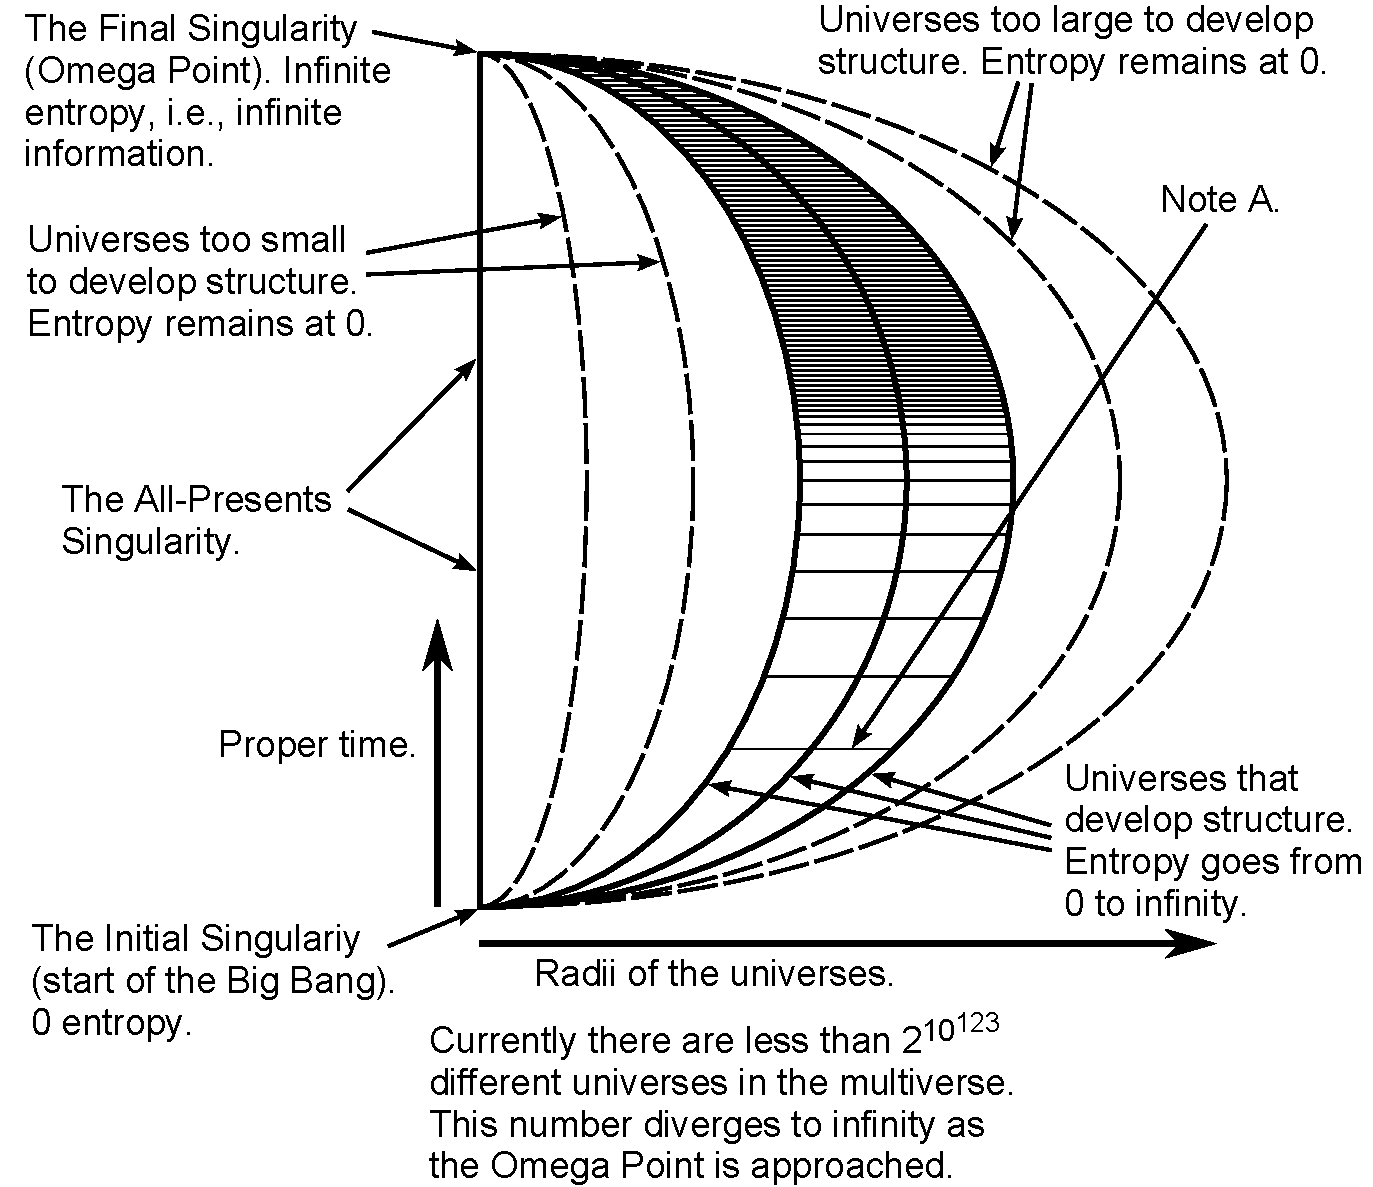
\includegraphics[width=0.8\textwidth]{Multiverse-Omega-Point.pdf}
  \caption[The Multiversal Formulation of the Omega Point Cosmology 1]{A diagram of the multiverse formulation of the Omega Point cosmology. Note that the physics of the Omega Point cosmology aren't dependent on a multiverse formulation. See also Figure \ref{fig:Circle-Multiverse-Omega-Point.pdf} on p. \pageref{fig:Circle-Multiverse-Omega-Point.pdf} for a different visualization of the multiversal Omega Point cosmology.\par\vspace{1em}
    \footnotesize\hspace{1em}\textbf{Note A:} Sapient life develops, gradually taking over control of more resources in the universes with structure, eventually becoming ubiquitous throughout and in control over all resources in each of these universes.\par
    \hspace{1em}During the colonization phase, life uses baryon annihilation for its energy requirements and for interstellar travel. In the process, the annihilation of baryons forces the Higgs field toward its absolute vacuum, thereby canceling the positive cosmological constant and forcing these universes to collapse.\par
    \hspace{1em}During the collapse phase, life in each of these universes uses energy from gravitational shear by forcing Taub universe collapses, thereby creating a temperature differential whereby usable energy can be obtained. The Taublike collapses, first in one direction, and then another direction (i.e., Mixmaster oscillations), are also used to eliminate event horizons, which is necessary for information processing (and hence life) to continue. This mode of collapse ends (in proper time) in a single \emph{c}-boundary (i.e., causal boundary) point: the Omega Point. The gravitational shear energy thereby available to life diverges to infinity as the Omega Point is approached.\par
    \hspace{1em}Due to the increasing temperature of these universes during the collapse phase (wherein the temperature diverges to infinity as the Omega Point is approached), life will have to transfer its information processes to higher energy states, eventually using elementary particles to directly compute on.}
  \label{fig:Multiverse-Omega-Point.pdf}
\end{figure}

\begin{figure}[htbp]
  \centering
    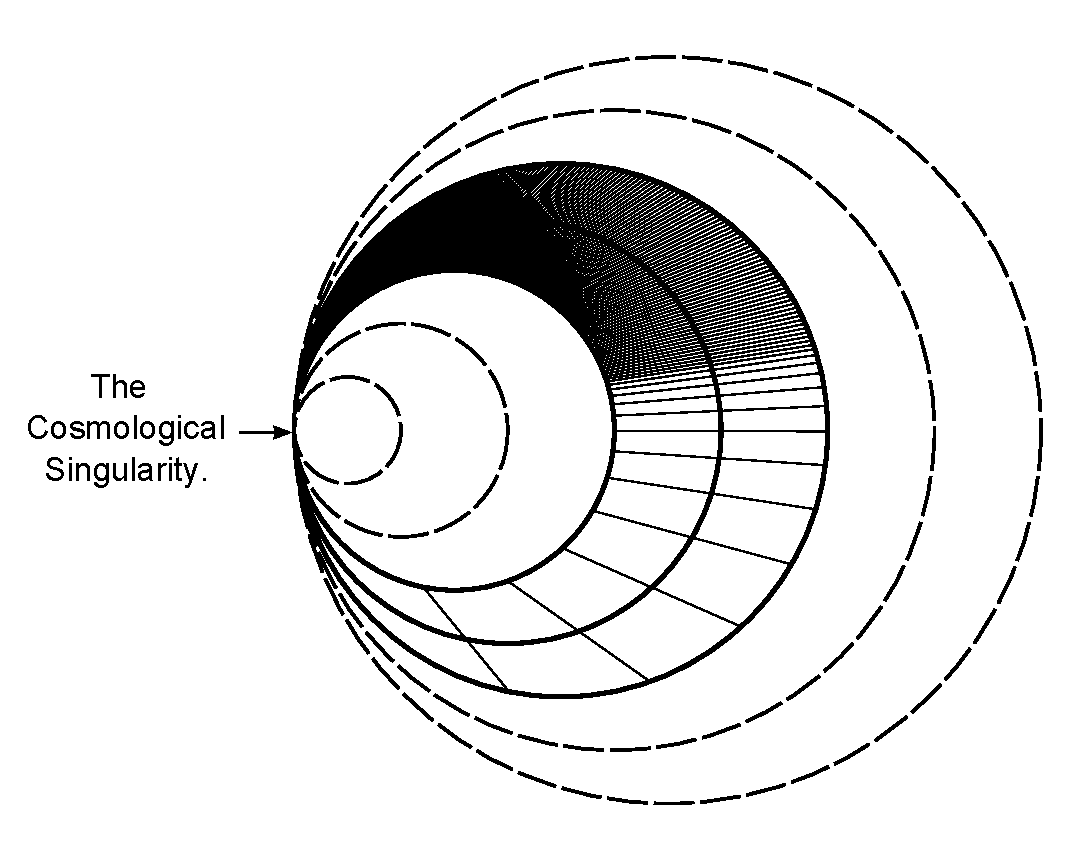
\includegraphics[width=0.7\textwidth]{Circle-Multiverse-Omega-Point.pdf}
  \caption[The Multiversal Formulation of the Omega Point Cosmology 2]{A diagram of the multiverse formulation of the Omega Point cosmology, here showing the unified nature of the Cosmological Singularity, with its different aspects being the Initial Singularity, the All-Presents Singularity and the Final Singularity, as depicted in Figure \ref{fig:Multiverse-Omega-Point.pdf} on p.~\pageref{fig:Multiverse-Omega-Point.pdf}. See also that diagram for an explanation of the other visual features of this diagram.}
  \label{fig:Circle-Multiverse-Omega-Point.pdf}
\end{figure}

In this book Tipler also analyzes how Jesus Christ could have performed the \glspl{miracle} attributed to him in the New Testament without violating any known laws of physics, even if one were to assume that we currently don't exist on a level of implementation in a computer simulation (in the case that we did, then such miracles would be trivially easy to perform for the society which was running the simulation, even though it would seem amazing from our perspective). This proposed process uses baryon annihilation, and its inverse, by way of electroweak quantum tunneling\footnote{\label{foot:BaryonMechanism}For the mechanism in the Standard Model of particle physics that allows for the nonconservation of baryon number (i.e., baryon annihilation, and its inverse, baryogenesis), see Refs. \citen{Hooft1976,ChengLi1984,RubakovShaposhnikov1996}; and \citen{Weinberg1996}, Ch. 23: ``Extended Field Configurations'', pp. 421--477. Weinberg gives a derivation of this mechanism from the Atiyah--Singer Index Theorem in Ref. \citen{Weinberg1996}. Gerardus 't Hooft, who discovered this new physical law in 1976 \cite{Hooft1976}, was awarded the Nobel Prize in Physics in 1999.} caused via the Principle of Least Action by the physical requirement that the Omega Point final cosmological singularity exists. Tipler also proposes that the virgin birth of Jesus by Mary could be possible via Jesus being a special type of XX male who obtained all of his genetic material from Mary (i.e., an instance of parthenogenesis). Tipler concludes that the Star of Bethlehem was either a Type Ic hypernova located in the Andromeda Galaxy, or a Type Ia supernova located in a globular cluster of our own Milky Way Galaxy.\footnote{Ref. \citen{Tipler2007}, Ch. 6: ``The Christmas Miracle: The Star of Bethlehem'', pp. 141--153, of which chapter is based upon Ref. \citen{Tipler2005-6}.}

If the Incarnation of Jesus Christ and the miracles attributed to him in the New Testament were necessary in order to lead to the formation of the Omega Point---and if the known laws of physics are correct---then the probability of these events occurring is certain. Furthermore, Tipler proposes tests on particular relics associated with Jesus which, if the relics are genuine, could verify whether in fact said miracles took place via the aforementioned mechanisms. Tipler writes in this book that miracles, if they indeed exist, do not violate physical law, but instead are events which are so improbable that they would only be likely to occur within human history via the Least-Action Principle if the universe is required to evolve into the Omega Point.

\emph{The Physics of Christianity} shows a change from Tipler's earlier position within \emph{The Physics of Immortality} regarding theism and Christianity. In the opening paragraph of Chapter XII: ``The Omega Point and Christianity'' of \emph{The Physics of Immortality}, Tipler wrote the following:\footnote{Ref. \citen{Tipler1994}, p. 305.}

\begin{squote}
To emphasize the scientific nature of the Omega Point Theory, let me state here that I am at present forced to consider myself an atheist, in the literal sense that I am not a theist. (\emph{A-theist} means ``not theist.'') I do not yet even believe in the Omega Point. The Omega Point Theory is a viable scientific theory of the future of the physical universe, but the only evidence in its favor at the moment is theoretical beauty, for there is as yet no confirming experimental evidence for it. Thus scientifically one is not compelled to accept it at the time of my writing these words. So I do not. [Antony] Flew, among others, has in my opinion made a convincing case for the presumption of atheism. If the Omega Point Theory and all possible variations of it are disconfirmed, then I think atheism in the sense of Flew, [David] Hume, [Bertrand] Russell, and the other self-described atheists is the only rational alternative. But of course I also think the Omega Point Theory has a very good chance of being right, otherwise I would never have troubled to write this book. If the Omega Point Theory is confirmed, I shall then consider myself a theist.
\end{squote}

Tipler is now a theist due to advancements in his Omega Point cosmology which occurred after the publication of \emph{The Physics of Immortality}.\footnote{Ref. \citen{Meddis1998}; see Part~1 concerning Tipler no longer being an atheist. And see Ref. \citen{Tipler2007}, p. 62.} Namely, Tipler has shown that the known laws of physics---specifically, the Second Law of Thermodynamics, General Relativity, and Quantum Mechanics---require the existence of the Omega Point singularity in order to avoid their violation \cite{Tipler1997,Tipler1998,TiplerEtAl2000,Tipler2000b,Tipler2001b,Tipler2003a,Tipler2003b,Tipler2005,Tipler2007}; whereas in \emph{The Physics of Immortality}, Tipler investigated what would be necessary from the postulate that life continues forever while still keeping the analysis confined to the known laws of physics.

These physical laws have been repeatedly confirmed by every experiment to date, constituting a massive body of empirical evidence for the Omega Point cosmology's correctness. And as indicated above, Tipler is also now a Christian due to the triune structure of the Omega Point cosmology preferentially selecting God as described by Christian theological tradition.

\section{Physics of the Omega Point Cosmology}
\label{sec:PhysicsOPT}

\subsection{The Omega Point}
\label{subsec:TheOmegaPoint}

From his 2005 paper in the journal \emph{Reports on Progress in Physics}, Prof. Tipler gives the following proof that the universe must end in the Omega Point in order for the known laws of physics (i.e., the Second Law of Thermodynamics, General Relativity, and Quantum Mechanics) to be mutually consistent at all times:\footnote{Ref. \citen{Tipler2005}, p. 925 of the \emph{Rep. Prog. Phys.} version; see also pp. 904--905. Citation formatting in the quoted passage has been modified for the sake of clarity, including the footnote numbers within superscript brackets that have been added by me. For this same proof given elsewhere by Tipler, see Refs. \citen{Tipler1997,Tipler1998,TiplerEtAl2000,Tipler2000b,Tipler2001b,Tipler2003a,Tipler2003b,Tipler2005,Tipler2007}.}

\begin{squote}
Astrophysical black holes almost certainly exist, but Hawking \cite{Hawking1976} and Wald\( ^[ \)\footnote{Ref. \citen{Wald1994}, Ch. 7: ``The Hawking Effect'', Sec. 7.3: ``Evaporation of Black Holes and Loss of Quantum Coherence'', pp. 175--187.}\( ^] \) have shown that if black holes are allowed to exist for unlimited proper time, then they will completely evaporate, and \gls{unitarity} will be violated. Thus, unitarity requires that the universe must cease to exist after finite proper time, which implies that the universe has spatial topology \glssymbol{S3}.\( ^[ \)\footnote{Tipler [\citen{Tipler2005}, p. 926 of the \emph{Rep. Prog. Phys.} version] writes that ``A dynamical proof for \glssymbol{S3} can be found in Barrow (1986)'', which is Ref. \citen{BarrowEtAl1986}.}\( ^] \) The Second Law of Thermodynamics says the amount of \gls{entropy} in the universe cannot decrease, but Ellis and Coule \cite{EllisCoule1994} and I\( ^[ \)\footnote{Ref. \citen{Tipler1994}, App.~C: ``The Bekenstein Bound'', pp. 410--411. Said Appendix is reproduced in Ref. \citen{Tipler2001b}, Sec. 2: ``Apparent Inconsistencies in the Physical Laws in the Early Universe'', Subsec. a: ``Bekenstein Bound Inconsistent with Second Law of Thermodynamics'', p.~7.}\( ^] \) have shown that the amount of entropy already in the \glslocalunset{CMBR}\gls{CMBR} will eventually contradict the \gls{BekensteinBound} near the final singularity unless there are no event horizons, since in the presence of horizons the Bekenstein Bound implies the universal entropy \( S \leq \text{constant [i.e., the Bekenstein Bound]} \times R^2 \), where \( R \) is the radius of the universe, and general relativity requires \( R \) \glssymbol{rightarrow} \( 0 \) at the final singularity. If there are no horizons then the (shear) energy density can grow as \( R^{-6} \) which means that the total available energy grows as \( (R^{-6})R^3 \sim R^{-3} \), and so the Bekenstein Bound yields \( ER \sim (R^{-3})R \sim R^{-2} \) which diverges as \( R^{-2} \) as \( R \) \glssymbol{rightarrow} \( 0 \) at the final singularity.\( ^[ \)\footnote{Ref. \citen{Tipler1994}, pp. 410--411 and 462. And Ref.  \citen{Tipler2003a}.}\( ^] \) The absence of event horizons by definition means that the universe's future c-boundary is a single point, call it the \emph{Omega Point}. MacCallum \cite{MacCallum1971} has shown that an \glssymbol{S3} closed universe with a single point future c-boundary is of measure zero in initial data space. Barrow \cite{Barrow1982,BarrowLevin1997}, Cornish and Levin \cite{CornisLevin1996} and Motter \cite{Motter2003} have shown that the evolution of an \glssymbol{S3} closed universe into its final singularity is chaotic. Yorke \emph{et al} \cite{ShinbrotEtAl1990,ShinbrotEtAl1992} have shown that a chaotic physical system is likely to evolve into a measure zero state if and only if its control parameters are intelligently manipulated. Thus life (\glssymbol{equiv}intelligent computers) almost certainly must be present \emph{arbitrarily close} to the final singularity in order for the known laws of physics to be mutually consistent at all times. Misner \cite{Misner1968,Misner1969-5,Misner1969-10} has shown in effect that event horizon elimination requires an infinite number of distinct manipulations, so an infinite amount of information must be processed between now and the final singularity. The amount of information stored at any time diverges to infinity as the Omega Point is approached, since \( S \) \glssymbol{rightarrow} \( +\infty \) there, implying divergence of the complexity of the system that must be understood to be controlled.
\end{squote}

\paragraph{Explanation of the Proof:}
\label{parag:ExplanationofProof}

Thus it's shown that the Omega Point cosmology is a logically-inescapable consequence of the known laws of physics.\footnote{Ergo, the title of Omega Point \emph{Theorem} is now correct to apply to the Omega Point cosmology, since it is now a mathematical theorem per the Second Law of Thermodynamics, General Relativity, and Quantum Mechanics. For more on this, see App. \ref{subsec:BekensteinBoundUltimateFutureUniverse}.} In the above, the phrase ``almost certainly'' (also called ``almost surely'' or ``with probability~1'') is a technical term in probability theory that means the likelihood of an event occurring has a probability of~1 (with the range of possible values being from 0 to~1 on the real line), i.e., that it is infinitely improbable that the event does not occur.\footnote{Ref. \citen{MSJ1993}, p. 1269.} However, another way to state the Second Law of Thermodynamics is that the universe evolves from less probable states to more probable states.\footnote{Ref. \citen{YourgrauEtAl2002}, Ch. 2: ``General Principles of Statistical Thermodynamics'', p. 94.} An infinitely improbable state is not a ``more probable'' state. Hence, in order for an infinitely improbable state to occur would require violation of the Second Law of Thermodynamics. Consequently, if the known laws of physics are true statements of how the world works, then the Omega Point cosmology is logically unavoidable.

In the above-quoted paragraph, ``measure zero'' is a technical term in measure theory (an area of mathematics which deals with the sizes of sets) that means ``null set'' (also called ``measure~0 set''). A null set corresponds to a probability of~0 in probability space, which in the above means that its occurrence is infinitely improbable if the selection-process is unguided.\footnote{Refs. \citen{Berry1978}, p. 73 (or p. 41 of the reprint); \citen{Gupta2006}, pp. 1--2.} Here the ``initial data space'' is the \emph{superset} in which this ``measure zero'' set exists. The initial data space is all the possible outcomes which could come about given particular physical conditions---the reason for it being called ``initial'' is because as time progresses, events occur which preclude other events from taking place.\footnote{Refs. \citen{Tipler1989}, p. 171 of the reprint; \citen{Tipler1994}, p. 161; \citen{BarrowTipler1986}, pp. 495--496, 501--502.} Hence, the \emph{initial} data space is the largest set of possible outcomes for a given physical system. In the context of the above, what it means is that the Omega Point cosmological singularity is infinitely improbable acting only on blind and dead forces, i.e., that the probability of the universe evolving into the Omega Point without intelligent control is infinitely improbable. The reason for this is because in order for the universe to evolve into the Omega Point, event horizons must be eliminated, otherwise one doesn't get a solitary-point final singularity (which is one of the definitions of the Omega Point), but instead a singularity with many different points due to different locations of the universe being out of causal contact with each other (which is what the term ``event horizon'' means), which would be completely lethal to life as eventually even a single computer with the complexity and intelligence of a human mind would be out of causal contact with the rest of itself, thereby making human-level intelligence impossible (and progressing further in time, eventually even the simplest form of life would become out causal contact with the rest of itself). Yet in order to eliminate event horizons requires intelligence to direct the collapse trajectories of the universe, necessitating an infinite number of distinct manipulations as the universe collapses toward the Omega Point. Because the complexity of the universe grows without bound, and because the universe must be understood so that its collapse trajectories can be controlled, life growing in intelligence without bound---becoming literally infinite in intelligence at the end of proper time---is a logically inherent consequence of the known laws of physics.\footnote{To elaborate on this matter, in order to eliminate event horizons life will have to understand the universe to \emph{some} degree. Life can't understand the universe in which it lives \emph{perfectly}, since that would involve a proper subset perfectly modeling its proper superset. Here the degree of life's understanding doesn't matter to this argument, as the issue is that the complexity of the universe is increasing, and this will necessarily increase the complexity of far-future life's imperfect models of how the universe is to evolve and thus how they are to respond to it so as to manipulate the universe's collapse trajectories---the point being here is that whatever their degree of understanding, said knowledge will still have to diverge to infinity.}

The phrase ``arbitrarily close'' in the foregoing block quotation of Tipler is a technical term in analysis (a branch of mathematics which includes calculus) that refers to the limit of a function. It means infinitesimally close, or infinitely close.\footnote{Ref. \citen{GowersEtAl2008}, Sec. 5.1: ``Limits'', p. 31.} The reason for this term being used here is because while the known laws of physics say that the cosmological singularity must exist, no possible laws of physics can apply to the singularity itself, because physical values are at infinity there, and hence it's not possible to perform the arithmetical operations of addition or subtraction (nor multiplication or division) on those physical values in order to apply a physics equation to them.

\paragraph{Further Elaboration:}
\label{parag:FurtherElaboration}

During the collapse phase of the universe, life obtains gravitational shear energy by forcing cycles of Taub universe collapses (named after physicist Abraham Haskel Taub\footnote{Refs. \citen{Taub1951,MisnerTaub1968,MacCallum2004,NewmanEtAl1963}; and \citen{RyanShepley1975}, Ch.~8: ``T--NUT--M Space---Open to Closed to Open'', pp. 132--146. Taub collapses have also been termed Kasner crushings, after mathematician Edward Kasner.}), whereby the universe collapses in one direction into the shape of an oblate spheroid by life directing trajectories of mass, thereby creating greater heating in the direction of collapse and hence a temperature differential whereby usable energy can be obtained.\footnote{Ref. \citen{Tipler1994}, pp. 136--144 and 462--463. This process which avoids Heat Death is depicted in Figure~\ref{fig:oblate-spheroid} on p. \pageref{fig:oblate-spheroid}.} The Taublike collapses, first in one direction, and then another direction (i.e., Mixmaster oscillations\footnote{Refs. \citen{Misner1968,Misner1969-5,Misner1969-10}. A Mixmaster universe is also called a Bianchi Type IX universe.}), are also used to eliminate event horizons by allowing communication across the universe in the direction of collapse, which is necessary for information processing (and hence life) to continue.\footnote{Black hole event horizons are eventually eliminated via the trapped surfaces of today's black holes merging with the future trapped surfaces of the collapsing universe. See Ref. \citen{Tipler1994}, App.~H: ``The Classical Omega Point Universe: Mathematical Details'', pp. 478--479. Cf. Ref. \citen{TiplerEtAl2000}, 2nd sentence of Sec.~6.} This mode of collapse ends (in proper time, as in computer clock time it never ends) in a single \emph{c}-boundary (i.e., causal boundary) point: the Omega Point. The gravitational shear energy thereby available to life diverges to infinity as the Omega Point is approached. That is, by making the negative gravitational energy go to minus infinity, the positive energy available to life goes to plus infinity, as the total energy of the universe at all times sums to exactly zero, as physicist Stephen Hawking has pointed out:\footnote{Ref. \citen{Hawking1996}, Ch.~8: ``The Origin and Fate of the Universe'', pp. 166--167.}

\begin{squotation}
The\refstepcounter{HawkingEnergyZ}\label{HawkingEnergy} answer [to where the universe's energy came from] is that the total energy of the universe is exactly zero. The matter in the universe is made out of positive energy. However, the matter is all attracting itself by gravity. Two pieces of matter that are close to each other have less energy than the same two pieces a long way apart, because you have to expend energy to separate them against the gravitational force that is pulling them together. Thus, in a sense, the gravitational field has negative energy. In the case of a universe that is approximately uniform in space, one can show that this negative gravitational energy exactly cancels the positive energy represented by the matter. So the total energy of the universe is zero.

Now twice zero is also zero. Thus the universe can double the amount of positive matter energy and also double the negative gravitational energy without violation of the conservation of energy.\thinspace\ldots\ As [physicist Alan] Guth has remarked, ``It is said that there's no such thing as a free lunch. But the universe is the ultimate free lunch.''
\end{squotation}

\begin{figure}[htbp]
  \centering
  \subfloat[]{\label{fig:oblate-spheroid-1.png}
\includegraphics[width=0.3\textwidth]{oblate-spheroid-1.png}}~
  \subfloat[]{\label{fig:oblate-spheroid-2.png}
\includegraphics[width=0.3\textwidth]{oblate-spheroid-2.png}}~
  \subfloat[]{\label{fig:oblate-spheroid-3.png}
\includegraphics[width=0.3\textwidth]{oblate-spheroid-3.png}}
  \caption[The Universe's Taublike Collapse Cycles]{2-Sphere representations of the universe during stages of one of its Taublike collapses. The actual spatial topology of the universe is that of a \protect\gls{3sphere}. The technical term for this squashed sphere shape is \emph{oblate spheroid}, which is a type of ellipsoid, and which has a 3-sphere analogue in addition to the 2-sphere form depicted above. In order to overcome event horizons so that light will circumnavigate the universe just once in the collapsing direction---hence allowing communication across the universe---the size of the universe in that direction must decrease by a factor of approximately 70 [\citen{Tipler1994}, p. 144], as depicted in frame~(c). Collapse in that direction is then halted and the universe undergoes collapse in a different direction, with an infinite number of these different Taublike collapses (i.e., Mixmaster oscillations) occurring before the final singularity, thereby allowing light to circumnavigate the universe an infinite number of times before the end of \protect\gls{propertime}, thus creating an infinite-communication universe whereby every point in the universe is able to signal to every other point in the universe an infinite number of times. These anisotropic collapse cycles additionally provide gravitational shear energy for life by creating a temperature differential across the universe, because greater heating occurs in the direction of collapse.}
  \label{fig:oblate-spheroid}
\end{figure}

The distance traversed in order for a signal (such as from a photon) to make a complete transition across the universe gets shorter and shorter as the universe collapses into the final singularity.\footnote{This process is depicted in the Penrose Diagram of Figure \ref{fig:Penrose-Omega-Point.pdf} on p. \pageref{fig:Penrose-Omega-Point.pdf}.} In other words, the universe's processor speed diverges toward becoming infinitely fast as the universe collapses into the singularity, as the amount of time it takes to send a signal across the universe is getting shorter. A light ray thereby traverses an infinite number of times across the entire universe before the final singularity, allowing an infinite number of computer clock cycles before the end of proper time. Hence, experiential time lasts forever, i.e., the number of thoughts that occur is infinite.

At the same time, the universe's entropy (i.e., informational complexity) diverges to infinity. In other words, the universe's memory space diverges to infinity at the same time that the universe's processor speed is diverging to infinity, with both becoming infinite at the final singularity (i.e., infinite processor speed and infinite memory space at the final singularity).

Some\refstepcounter{UniverseAccelerationZ}\label{UniverseAcceleration} have suggested that the current acceleration of the universe's expansion due to the positive cosmological constant would appear to obviate the Omega Point. Although physicists Profs. Lawrence M. Krauss and Michael S. Turner have pointed out \cite{Krauss1999} that

\begin{squote}
The recognition that the cosmological constant may be non-zero forces us to re-evaluate standard notions about the connection between geometry and the fate of our Universe. An open Universe can recollapse, and a closed Universe can expand forever. As a corollary, we point out that there is no set of cosmological observations we can perform that will unambiguously allow us to determine what the ultimate destiny of the Universe will be.
\end{squote}

The reason why cosmological observations cannot tell us whether the universe will expand forever or eventually collapse is because that is dependent on the actions of intelligent life. The known laws of physics provide the mechanism for the universe's collapse. As required by the Standard Model of particle physics, the net baryon number was created in the early universe by baryogenesis via electroweak quantum tunneling. This necessarily forces the Higgs field to be in a vacuum state that is not its absolute vacuum, which is the cause of the observed cosmological constant. But by sapient life annihilating baryons in the universe---again via electroweak quantum tunneling (which is allowed in the Standard Model, as baryon number minus lepton number, \( B-L \), is conserved\footnote{Again, see footnote \ref{foot:BaryonMechanism} on p. \pageref{foot:BaryonMechanism} for the details of this mechanism.})---the Higgs field is forced toward its absolute vacuum state, canceling the observed cosmological constant and thereby allowing the universe to collapse. Moreover, this process will provide the ideal form of energy resource and rocket propulsion during the colonization phase of the universe. As Tipler writes:\footnote{Ref. \citen{Tipler2003b}. Citation numbering in the quoted passage has been modified for the sake of clarity. See also Refs. \citen{Tipler2001b,Tipler2003a,Tipler2005,Tipler2007} for more on this mechanism of the universe's collapse. In his 1994 book, Tipler recognized that the Higgs field could stop the collapse of the universe but did not at the time investigate the full implications of this [\citen{Tipler1994}, p. 465; cf. p. 150]: ``The only known mechanism that could stop the contraction [of the universe] is the positive cosmological constant \( \Lambda \) [Lambda] that must exist (if the standard model is correct) to cancel the current negative energy density of the Higgs field;~\ldots''.}

\begin{squote}
The \glslocalunset{SM}\gls{SM} provides such a mechanism, which I actually discussed in the last section of the Appendix for Scientists in (\cite{Tipler1994}, p. 515). This mechanism is the creation\slash destruction of baryon number by electroweak quantum tunneling. (Baryons are the heavy particles made up of quarks. Examples are neutrons and protons.) In my book, I pointed out that this mechanism would be ideal for propelling interstellar spacecraft, but I did not discuss its implications for the Higgs vacuum, a serious oversight on my part. (An oversight which invalidates the second part of my Fifth Prediction on page 149 of \cite{Tipler1994}.) If the \gls{SM} is true---ALL experiments conducted to date indicate that it is (e.g. \cite{Wilczek2002} and \cite{Quinn2003}, last full paragraph on p.~35)---then the net baryon number observed in the universe must have been created in the early universe by this mechanism of electroweak quantum tunneling. If the baryons were so created, then this process necessarily forces the Higgs field to be in a vacuum state that is not its absolute vacuum. But if the baryons in the universe were to be annihilated by this process, say by the action of intelligent life, then this would force the Higgs field toward its absolute vacuum, canceling the positive cosmological constant, stopping the acceleration, and allowing the universe to collapse into the Omega Point. Conversely, if enough baryons are not annihilated by this process, the positive cosmological constant will never be cancelled, the universe will expand forever, unitarity will be violated, and the Omega Point will never come into existence. Only if life makes use of this process to annihilate baryons will the Omega Point come into existence.
\end{squote}

\begin{figure}[htbp]
  \centering
    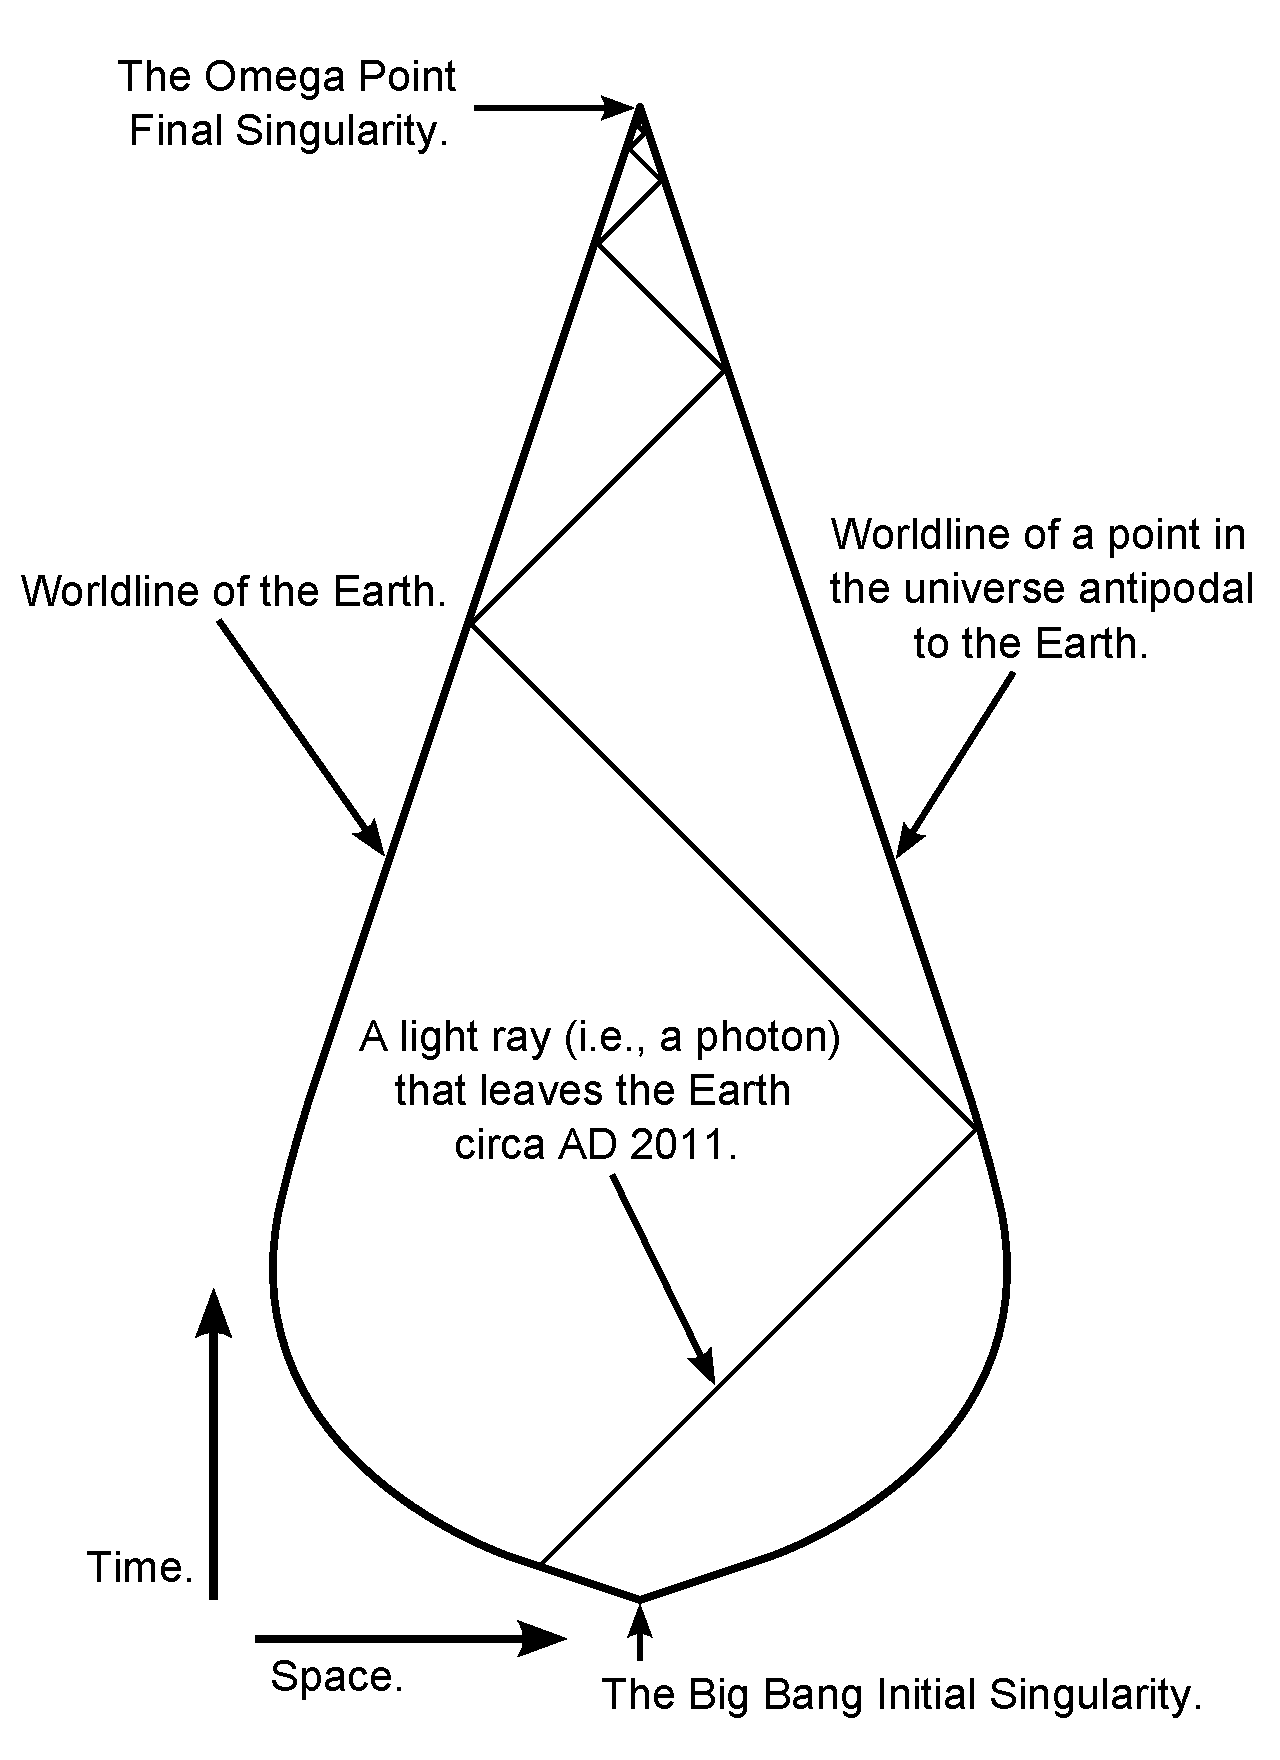
\includegraphics[width=0.6\textwidth]{Penrose-Omega-Point.pdf}
  \caption[Penrose Diagram of the Omega Point Cosmology]{A Penrose Diagram (named after physicist Roger Penrose \cite{Tipler1987}) of the Omega Point cosmology, showing the \emph{c}-boundary (i.e., causal boundary) of a solitary-point final singularity, termed the Omega Point. A photon traverses the entire length of the universe an infinite number of times before the final singularity is reached. Furthermore, the distance between antipodal points in the universe becomes closer and closer as the universe collapses into the final singularity, meaning that the time it takes a photon to travel between opposite points of the universe becomes shorter and shorter, i.e., the time it takes to send a signal between different points in the universe is decreasing. In other words, an infinite number of computer processor cycles occur before the final singularity (i.e., an infinite number of bits are processed, i.e., an infinite number of thoughts occur), and the processor speed of the universe diverges to infinity as the universe collapses into the final singularity.} 
  \label{fig:Penrose-Omega-Point.pdf}
\end{figure}

\begin{figure}[htbp]
  \centering
    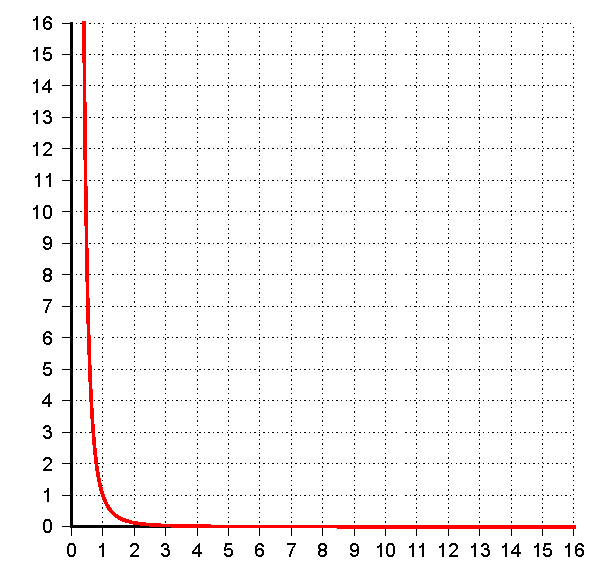
\includegraphics[width=0.66666667\textwidth]{Universe-Energy.pdf}
  \caption[Available Energy During the Universe's Collapse]{Total available energy as the radius of the universe goes to zero: \( E = R^{-6}\times R^3 = R^{-3} = 1/R^3 \). That is, for every halving of the universe's radius \( R \), the total available energy \( E \) increases by 8 times. In the graph, the horizontal axis is the radius, and the vertical axis is the energy. The limit of this function is \( \lim_{R\searrow 0}\frac{1}{R^3} = +\infty\times E \).}
  \label{fig:Universe-Energy.pdf}
\end{figure}

\begin{figure}[htbp]
  \centering
    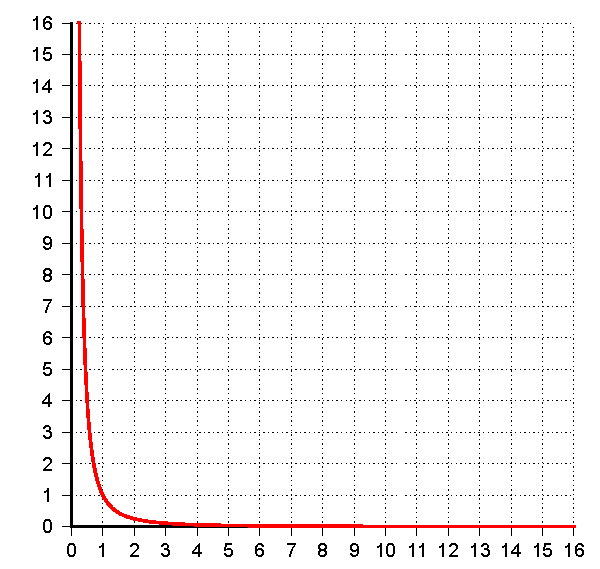
\includegraphics[width=0.66666667\textwidth]{Universe-Entropy.pdf}
  \caption[Entropy Growth Allowed During the Universe's Collapse]{Entropy growth allowed by the Bekenstein Bound as the radius of the universe goes to zero: \( S \leq R^{-3}\times R = R^{-2} = 1/R^2 \). That is, for every halving of the universe's radius \( R \), the entropy \( S \) allowed by the Bekenstein Bound can increase by 4 times. In the graph, the horizontal axis is the radius, and the vertical axis is the entropy.}
  \label{fig:Universe-Entropy.pdf}
\end{figure}

\subsection{The Omega Point and the Quantum Gravity Theory of Everything}
\label{subsec:OPQuantumGravityTOE}

In his 2005 paper in the journal \emph{Reports on Progress in Physics} \cite{Tipler2005}, Tipler demonstrates that the correct\footnote{That is, correct according to the known laws of physics.} quantum gravity theory has existed since 1962, first discovered in that year by Richard Feynman \cite{Feynman1963,Feynman1995,Feynman1972a,Feynman1972b} (awarded the 1965 Nobel Prize in Physics), and further independently developed by Bryce DeWitt \cite{DeWitt1967-8,DeWitt1967-10a,DeWitt1967-10b,DeWitt1968}, Steven Weinberg \cite{Weinberg1979} (awarded the 1979 Nobel Prize in Physics), and others \cite{FaddeevPopov1967,Mandelstam1968a,Mandelstam1968b,FradkinTyutin1970}. But because these physicists were looking for equations with a finite number of terms (i.e., differential equations with derivatives no higher than second order), they abandoned this qualitatively unique quantum gravity theory since in order for it to be consistent it requires an arbitrarily higher number of terms \cite{Tipler2007}. ``They also did not realize that the correct quantum gravity theory is consistent only if a certain set of boundary conditions are imposed~\ldots'', writes Tipler (which includes the initial Big Bang, and the final Omega Point, cosmological singularities).\footnote{Ref. \citen{Tipler2005}, p. 899 of the \emph{Rep. Prog. Phys.} version.} The equations for this theory of quantum gravity are term-by-term finite, but the same mechanism that forces each term in the series to be finite also forces the entire series to be infinite (i.e., infinities that would otherwise occur in spacetime, consequently destabilizing it, are transferred to the cosmological singularities, thereby preventing the universe from immediately collapsing into nonexistence\footnote{On this matter, see Refs. \citen{BarrowTipler1987,Tipler1986b}, in addition to Tipler's 2005 \emph{Rep. Prog. Phys.} paper \cite{Tipler2005} and his 2007 book \cite{Tipler2007}.}). Tipler writes that\footnote{Ref. \citen{Tipler2007}, p. 49, and the endnote on p. 279 to the sentence before the ellipsis.}

\begin{squotation}
It is a fundamental mathematical fact that this [infinite series] is the best that we can do.\thinspace\ldots

This is somewhat analogous to Liouville's theorem in complex analysis, which says that all analytic functions other than constants have singularities either a finite distance from the origin of coordinates or at infinity.
\end{squotation}

From the aforesaid \emph{Reports on Progress in Physics} paper, Tipler elaborates on the mathematics and physics of this issue, in part explained below:\footnote{Ref. \citen{Tipler2005}, p. 914 of the \emph{Rep. Prog. Phys.} version. Citation formatting in the quoted passage has been modified for the sake of clarity. Typographical errors in this quoted passage have been corrected, again for clarity.}

\begin{squotation}
So basic quantum field theory quickly forces upon us the general invariant action \begin{align*}
S = \int d^4x\, \sqrt{-g}\bigg(\Lambda + \frac{1}{8\pi G}R + c^2_1R^2 + c^3_1R^3 \cdots\nonumber\\
+\ c^2_2R_{\mu\nu}R^{\mu\nu} + \cdots + c^3_1R_{\mu\nu;\alpha}R^{\mu\nu;\alpha} + \cdots\bigg)
\tag{3}
\label{eq:gravS}
\end{align*}

This is the qualitatively unique gravitational Lagrangian picked out by quantum mechanics. Physicists do not like it because (1) it has an infinite number of (renormalizable) constants \( c^i_j \), all of which must be determined by experiment and (2) it will it not yield second order differential equations which all physicists know and love. But the countable number of constants are in effect axioms of the theory, and I pointed out in an earlier section that the L\"owenheim--Skolem theorem suggests there is no real difference between a theory with a countable number of axioms and a theory with a finite number of axioms. The finite case is just easier for humans to deal with, provided the `finite' number is a small number. Further, as Weinberg (\cite{Weinberg1995}, pp 499, 518--519) has emphasized, this Lagrangian generates a quantum theory of gravity that is just as renormalizable as \glslocalunset{QED}\gls{QED} and the \gls{SM}.

Since quantum field theory itself is forcing the Lagrangian (\ref{eq:gravS}) on us, I propose that we accept the judgement of quantum mechanics and accept (\ref{eq:gravS}) (and the countable number of additional terms involving the non-gravitational fields interacting with the \( h_{\mu\nu} \)) as the actual Lagrangian of reality.

Donoghue \cite{Donoghue1994} and Donoghue and Torma \cite{DonoghueTorma1996} have shown that Lagrangian (\ref{eq:gravS}) will not contradict experiment provided the (renormalized) values of the infinite number of new coupling constants are sufficiently small.\thinspace\ldots
\end{squotation}

One consequence of the above Lagrangian being the true description of quantum gravity is that so long as one is within spacetime, then one can never obtain a \emph{complete} description of quantum gravity and hence of physics: there will always be infinitely more to learn and discover in the field of physics, including by requiring the use of experiment \cite{Tipler2007}. Physics will become ever-more refined, knowledgeable and precise, but never complete (i.e., within spacetime). Only at the final singularity of the Omega Point (which is not in spacetime\footnote{Ref. \citen{HawkingEllis1973}, Ch.~6: ``Causal structure'', Sec. 6.8: ``The causal boundary of space-time'', pp. 217--221.}) will the full description of physics be obtained.

In the same journal article, Tipler combines the above theory of quantum gravity with the extended Standard Model of particle physics in order to form the Theory of Everything (\textsc{toe}) correctly describing and unifying all the forces in physics.\footnote{See also Refs. \citen{Tipler2001b,Tipler2005,Tipler2007} for where Tipler has described the Omega Point \textsc{toe} elsewhere.}

The Feynman--DeWitt--Weinberg quantum gravity\slash Standard Model \textsc{toe} solves all the outstanding problems in physics and cosmology, such as the black hole information issue; the dark matter and the dark energy; the observed isotropy, homogeneity, and spatial flatness of the universe; the observed excess of matter over antimatter; the observed photon to baryon ratio; the Harrison--Zel'dovich perturbation spectrum; the Greisen--Zatsepin--Kuzmin Ultra-High-Energy Cosmic Rays issue; the Gauge Hierarchy Problem; the free parameters to the Standard Model; etc.

Out of 50 articles, Tipler's said paper was selected \cite{Palmer2006} as one of 12 for the ``Highlights of 2005'' accolade as

\begin{squote}
the very best articles published in \emph{Reports on Progress in Physics} in 2005 [Vol. 68]. Articles were selected by the Editorial Board for their outstanding reviews of the field. They all received the highest praise from our international referees and a high number of downloads from the journal Website.
\end{squote}

\emph{Reports on Progress in Physics} is the leading peer-reviewed journal of the Institute of Physics, Britain's main professional body for physicists. Further, \emph{Reports on Progress in Physics} has a higher impact factor (according to \emph{Journal Citation Reports}\footnote{Refs. \citen{CSIR2007}; and \citen{IOPPublishing2008}, p. 37.}) than \emph{Physical Review Letters}, which is the most prestigious American physics journal (one, incidently, which Prof. Tipler has been published in more than once). A journal's impact factor is a measure of the importance the science community places in that journal in the sense of actually citing its papers in their own papers, with a higher number meaning more citations. Impact factors published by \emph{Journal Citation Reports} are the standard measure used to compare a journal's influence.

\subsection{The Universal Resurrection of the Dead}
\label{subsec:UniversalResurrectionOfTheDead}

Given an infinite amount of computational resources, recreating the exact quantum state of our present universe is trivial (per the \gls{BekensteinBound}), requiring at most a mere \( 10^{123} \) bits (the number which Roger Penrose calculated), or at most a mere \( 2^{10^{123}} \) bits for every different quantum configuration of the universe logically possible (i.e., the powerset, of which the multiverse in its entirety at this point in universal history is a proper subset of this powerset).\footnote{Ref. \citen{Tipler2005}, pp. 903--904 of the \emph{Rep. Prog. Phys.} version.} So the Omega Point will be able to resurrect us using merely an infinitesimally small amount of total computational resources: indeed, the multiversal resurrection will occur between \( 10^{-10^{10}} \) and \( 10^{-10^{123}} \) seconds before the Omega Point is reached, as the computational capacity of the universe at that stage will be great enough that doing so will require only a trivial amount of total computational resources.\footnote{Ref. \citen{Tipler1994}, Ch. IX: ``The Physics of the Resurrection of the Dead to Eternal Life'', Sec.: ``When Will the Dead Be Raised?'', pp. 225.}

\paragraph{The Continuity of Consciousness:}
\label{parag:ContinuityOfConsciousness}

Logically speaking, an exact emulation \emph{is} the thing being emulated. If it were not, then this would violate the Law of Identity in the field of logic, and thus it would be a logical contradiction. An exact emulation of, e.g., a human is merely a very large number.\footnote{For the details on this, see App.~\ref{sec:BekensteinBound}.} Indeed, even the entire lifetime of a human can be perfectly described by a single number---a tremendously large number compared to the numbers we're used to dealing with, but still quite finite.

To say that a perfect emulation is \emph{not} the thing being emulated would be the same as saying that 3765258724 \( \neq \) 3765258724, i.e., that there is something about the number 3765258724 on the left-hand side of the foregoing relation which makes it nonequivalent to the version on the right-hand side. But this is a logical contradiction, as it violates the Law of Identity that \( A = A \).

So as conclusively as one can maintain that \( A = A \) (and one can be logically certain of this), then one can be confident that one's resurrected self will \emph{be} oneself in every possible way, and that one's consciousness will continue. Again, to suppose otherwise involves a logical contradiction.

\subsection{The Omega Point Cosmology Vis-\`{a}-Vis String Theory and Other Proposed New Physics}
\label{subsec:StringTheory}

According to string theorist Prof. Brian Greene, it is unknown if singularities of gravitational collapse are possible or excluded in String Theory as applied to the actual geometry of the universe, although he states that string theorists suspect that no object can be compressed below the Planck length within String Theory.\footnote{Ref. \citen{Greene1999}, Ch. 10: ``Quantum Geometry'', Sec.: ``How General Is This Conclusion?'', pp. 254--255; cf. pp. 236, 239, 252--255 and 357--358.} If such singularities are not possible in String Theory, then String Theory would violate the known laws of physics in this regard, specifically General Relativity (for details on this, see the discussion regarding the Penrose--Hawking--Geroch Singularity Theorems in Section~\ref{sec:BigBang}). As well, the Omega Point cosmology requires the existence of a cosmological singularity at the end of proper time, and the Omega Point cosmology is required by the known laws of physics.

Prof. Stephen Hawking has proposed \cite{Hawking2005} a solution to the black hole information issue in order to preserve unitarity but without the universe collapsing which is dependent on the conjectured String Theory-based anti-de Sitter space\slash conformal field theory correspondence (AdS\slash CFT correspondence). Besides proposing new physical laws that have no experimental confirmation in an effort to solve the black hole information problem, Hawking's proposal also violates the known laws of physics (see Appendix \ref{subsec:BekensteinBoundUltimateFutureUniverse} for the details on that).

Whereas the known laws of physics have been confirmed by every experiment conducted to date, String Theory has never been confirmed by even a single experiment. As yet, String Theory has been nothing more than pure mathematics with the aspiration held by its proponents of someday becoming physics---a goal that has so far been a wild-goose chase. Tipler himself argues against the validity of String Theory in its current state \cite{Tipler2005}. The same lack of experimental confirmation presently applies to all other forms of proposed new physics, and such proposed new physics also violate the known laws of physics.

\section{Criticisms of the Omega Point Cosmology}
\label{sec:Criticisms}

To date the only peer-reviewed paper in a physics journal that has criticized Tipler's Omega Point cosmology has been in 1994 by physicists Prof. George Ellis and Dr. David Coule in the journal \emph{General Relativity and Gravitation} \cite{EllisCoule1994}. In the paper, Ellis and Coule unwittingly gave an argument that the Bekenstein Bound violates the Second Law of Thermodynamics if the universe collapses without having event horizons eliminated.\footnote{See Ref. \citen{EllisCoule1994}, p. 733, Equation No.~3, and the discussion by Tipler on this paper in Ref. \citen{Tipler1994}, pp. 410--411.} Yet in order to bring about the Omega Point, event horizons must be eliminated, and Tipler cites this paper in favor of the fact that the known laws of physics require the Omega Point to exist.\footnote{Ref. \citen{Tipler2005}, p. 925 of the \emph{Rep. Prog. Phys.} version.}

There have also been a number of unrefereed book reviews appearing in science journals and popular science magazines which have been critical of Tipler's Omega Point cosmology. Writing in the ``Book Reviews'' section of the journal \emph{Nature}, Ellis \cite{Ellis1994} described Tipler's book \emph{The Physics of Immortality} as ``a masterpiece of pseudoscience.\thinspace\ldots\ the product of a fertile and creative imagination unhampered by the normal constraints of scientific or philosophical discipline.'' Ellis's criticisms in his review consist of the logical fallacy of bare assertion while ignoring what Tipler actually wrote. If one ignores what the critiqued individual wrote then one can construct any irrelevant objection.

For example, Ellis asserts that Tipler ``ignores the fact'' that life cannot exist at arbitrarily high temperatures, but it is Ellis who ignores the fact that Tipler already addressed this matter in the very book under review. Physics allows life to exist as the temperature diverges to infinity if enough energy is available in which to record processed information (i.e., store manipulated bits) and the information-bearing medium exists at an energy level high enough in which to store information at the given temperatures. Tipler points out in his said book that such energy will be available and that within the Omega Point cosmology the energy levels for the medium in which to store information at the given temperatures automatically scale with the collapse of the universe.\footnote{Ref. \citen{Tipler1994}, pp. 461--463, 465, 473 and 475--476. See also Ref. \citen{Tipler2005}.} It's as if Ellis skimmed parts of the book without reading all of it, and hence is unaware that his objections were already addressed.\footnote{Ellis elsewhere \cite{StoegerEllis1995} makes this same faulty criticism, also with no apparent awareness that Tipler already addressed this matter.}

In the magazine \emph{New Scientist}, physicist Prof. Lawrence M. Krauss \cite{Krauss2007} referred to Tipler's book \emph{The Physics of Christianity} as ``a collection of half-truths and exaggerations, I am tempted to describe Tipler's new book as nonsense---but that would be unfair to the concept of nonsense. It is far more dangerous than mere nonsense~\ldots''. Elsewhere, Krauss has made it a point to emphasize what he considers to be the utter purposelessness of the universe and the futility of human life within in.\footnote{Ref. \citen{Krauss2009}, 43:10 min:sec ff. At 55:53 min:sec ff., Krauss uses an invective to refer to Tipler.} It's quite bizarre then how Tipler's writings could possibly be viewed as ``dangerous'' by Krauss, since per Krauss's \emph{Weltanschauung}, existence is completely pointless. Apparently Krauss believes that Tipler's ``dangerous'' ideas pose the risk of screwing up mankind's pointless fate!

In his review, Krauss repeatedly commits the logical fallacy of bare assertion. Krauss gives no indication that he followed up on the endnotes in the book \emph{The Physics of Christianity} and actually read Tipler's physics journal papers. All that Krauss is going off of in said review is Tipler's mostly nontechnical popular-audience book \emph{The Physics of Christianity} without researching Tipler's technical papers in the physics journals. Krauss's review offers no actual lines of reasoning for Krauss's pronouncements. His readership is simply expected to imbibe what Krauss proclaims, even though it's clear that Krauss is merely critiquing a popular-audience book which does not attempt to present the rigorous technical details.

For instance, Krauss asserts that ``He [Tipler] claims that we have a clear and consistent theory of quantum gravity. We don't.'' Whereas Tipler gives detailed arguments for the Omega Point\slash Feynman--DeWitt--Weinberg quantum gravity\slash Standard Model Theory of Everything (\textsc{toe}) in his 2005 \emph{Reports on Progress in Physics} paper \cite{Tipler2005}. Krauss displays no awareness of this peer-reviewed paper or of Tipler's other refereed papers on the Omega Point cosmology published in many physics journals.

Although in this same review, Krauss does admit that the mechanism that Tipler proposes for Jesus Christ's \glspl{miracle} is physically sound if said miracles were necessary in order to lead to the formation of the Omega Point and if the Omega Point is required in order for existence to exist.

Ironically, Krauss has actually published a paper that greatly helped to strengthen Tipler's Omega Point cosmology. Some have suggested that the current acceleration of the universe's expansion due to the positive cosmological constant would appear to obviate the Omega Point. However, Profs. Krauss and Michael S. Turner point out in Reference \citen{Krauss1999} that ``there is no set of cosmological observations we can perform that will unambiguously allow us to determine what the ultimate destiny of the Universe will be.''

As pointed out with Ellis and Coule's criticism, this isn't the first time that this ironic outcome has befallen critics of Tipler's Omega Point cosmology. So when Tipler's critics actually do real physics instead of issuing bare assertions and \emph{nihil ad rem} cavils, they end up making Tipler's case stronger. Ironic though it is, nevertheless that's the expected result, since the Omega Point cosmology is required by the known laws of physics.

\section{The Big Bang}
\label{sec:BigBang}

Physics, in the form of the Big Bang cosmology, has many decades ago already demonstrated per the known laws of physics that God exists, since the Big Bang singularity is the first cause, one of the ancient definitions of God held by all the Abrahamic religions.

Unfortunately, most modern physicists have been all too willing to abandon the laws of physics if it produces results that they're uncomfortable with, i.e., in reference to religion. It's the antagonism for religion on the part of the scientific community which greatly held up the acceptance of the Big Bang (for some 40 years), due to said scientific community's displeasure with it confirming the traditional theological position of \emph{creatio ex nihilo}, and also because no laws of physics can apply to the singularity itself: i.e., quite literally, the singularity is \gls{supernatural}, in the sense that no form of physics can apply to it, since physical values are at infinity at the singularity, and so it is not possible to perform arithmetical operations on them; and in the sense that the singularity is beyond creation, as it is not a part of spacetime, but rather is the boundary of space and time.\footnote{Ref. \citen{HawkingEllis1973}, Ch.~6: ``Causal structure'', Sec. 6.8: ``The causal boundary of space-time'', pp. 217--221.}

The originator of the Big Bang theory was Roman Catholic priest and physicist Prof. Georges Lema\^{i}tre in 1927;\footnote{Refs. \citen{Lemaitre1927,Lemaitre1931a,Lemaitre1931b,Lemaitre1933,Lemaitre1934}. Alexander Friedmann was the first to derive solutions to Einstein's field equations that require the curvature of space to vary with time \cite{Friedmann1922,Friedmann1924}, but did not suggest that the universe was actually expanding. Lema\^{i}tre independently derived the solutions, and proposed that the universe was in fact expanding (as also the title to his first paper \cite{Lemaitre1927} on the subject indicates), while providing observational evidence that this was so. For histories on this, see Refs. \citen{Blanchard2001,Kragh2003,McVittie1967}. As physicist George C. McVittie wrote [\citen{McVittie1967}, p. 296] in the \emph{Quarterly Journal of the Royal Astronomical Society}'s obituary for Lema\^{i}tre, \begin{quote}
It is true that, unknown to Lemaitre, the Russian mathematician A.~Friedmann had, in 1922 and 1924, published papers in which the general differential equation for [Einstein's field equations' radial scale-factor] \( R \) was considered. But Lemaitre went beyond the determination of a specific form for \( R \): he showed that his model could be used to interpret the observed redshift in the spectra of extragalactic nebulae, regarded as a Doppler effect. With this step, cosmology, as we know it today, was launched.
\end{quote} And as physicist Alain Blanchard wrote [\citen{Blanchard2001}, p. 241], \begin{quote}
the questions he [Lema\^{i}tre] addressed shows that he was the first cosmologist in the modern sense \ldots\ In this sense, [according] to [cosmologist] Jim Peebles, Physical Cosmology during the century was essentially a continuation of Lema\^{i}tre's program (Peebles, 1991).
\end{quote} Wherein ``(Peebles, 1991)'' is Ref. \citen{Peebles1991}.} and it was enthusiastically endorsed by Pope Pius XII in 1951, long before the scientific community finally came to accept it. Indeed, Lema\^{i}tre relates that when he spoke with Albert Einstein regarding his Primaeval Atom Hypothesis, Einstein's response to it was \emph{``Non, pas cela, cela sugg\`{e}re trop la cr\'{e}ation''} (``No, not this---this too much suggests the creation'').\footnote{Ref. \citen{Lemaitre1958-01}. Lema\^{i}tre's meaning of \emph{``atome primitif''} is the initial cosmological singularity of zero radius, with ``atom'' being used in the ancient Greek sense of Leucippus and Democritus as an indivisible unity [\citen{Lemaitre1958}, p. 477]. Lema\^{i}tre's Primaeval Atom Hypothesis would later be mathematically proved per General Relativity with the Penrose--Hawking--Geroch Singularity Theorems, discussed in this section farther below.}

Genesis 1:1 and John 1:1--5 assert that the universe had a beginning, and that God is its First Cause.\footnote{Cf. 2~Maccabees 7:28.} Rabbi Moses Maimonides,\footnote{Ref. \citen{MaimonidesPerplexed}, Part~1, Ch. 69, pp. 102--105, passim.} and Thomas Aquinas in his Five Ways,\footnote{Ref. \citen{ThomasTheologiae}, 1st Part, Question~2, Art.~3.} had both defined God as the uncaused First Cause,\footnote{Interestingly, the First Cause does have a cause in the sense of future-to-past causality. However, in past-to-future causality, all causal chains begin at the Big Bang initial singularity, and so it is uncaused in the sense of how humans commonly think of causality. Another sense in which the cosmological singularity is uncaused is that it is outside of spacetime [\citen{HawkingEllis1973}, pp. 217--221], and therefore eternal, as time does not apply to it.} which is equivalent to Aristotle's conception of God as the Unmoved First Mover (i.e., the Prime Mover).\footnote{Ref. \citen{AristotleMetaphys}, Book 12 (\( \Lambda \)), Ch.~7, Bekker Nos. ca. 1072a20--1073a10.} The physics community was therefore quite reluctant to confirm with the Big Bang that God exists per this traditional and ancient definition of God.

As regards physicists abandoning physical law due to their theological discomfort with the Big Bang cosmology, in an article by Prof. Tipler he gives the following example involving no less than physicist Prof. Steven Weinberg:\footnote{Ref. \citen{Tipler2003a0}. In the quoted passage, the footnote number within the superscript brackets was added by me. Also see Ref. \citen{Tipler2003a0} for a number of other such examples of physicists rejecting physical law if it conflicts with their distaste for religion.}

\begin{squotation}
The most radical ideas are those that are perceived to support religion, specifically Judaism and Christianity. When I was a student at MIT in the late 1960s, I audited a course in cosmology from the physics Nobelist Steven Weinberg. He told his class that of the theories of cosmology, he preferred the Steady State Theory because ``it \emph{least} resembled the account in Genesis'' (my emphasis). In his book \emph{The First Three Minutes} (chapter 6),\( ^[\footnote{Ref. \citen{Weinberg1977}.}^] \) Weinberg explains his earlier rejection of the Big Bang Theory: ``[O]ur mistake is not that we take our theories too seriously, but that we do not take them seriously enough. It is always hard to realize that these numbers and equations we play with at our desks have something to do with the real world. \emph{Even worse, there often seems to be a general agreement that certain phenomena are just not fit subjects for respectable theoretical and experimental effort.}'' [My emphasis---J.~R.]

I have now known Weinberg for over thirty years, and I know that he has \emph{always} taken the equations of physics very seriously indeed. He and I are both convinced that the equations of physics are the best guide to reality, \emph{especially} when the predictions of these equations are contrary to common sense. But as he himself points out in his book, the Big Bang Theory was an automatic consequence of standard thermodynamics, standard gravity theory, and standard nuclear physics. All of the basic physics one needs for the Big Bang Theory was well established in the 1930s, some two decades before the theory was worked out. Weinberg rejected this standard physics not because he didn't take the equations of physics seriously, but because he did not like the religious implications of the laws of physics.\thinspace\ldots
\end{squotation}

Prof. Stephen Hawking reinforces what Einstein, Weinberg and Tipler spoke about concerning the antagonism of the 20th century scientific community for religion, resulting in the scientific community abandoning good physics. In his famous book \emph{A Brief History of Time}, Hawking wrote that\footnote{Ref. \citen{Hawking1996}, p. 62.}

\begin{squote}
Many people do not like the idea that time has a beginning, probably because it smacks of divine intervention. (The Catholic Church, on the other hand, seized on the big bang model and in 1951 officially pronounced it to be in accordance with the Bible). There were therefore a number of attempts to avoid the conclusion that there had been a big bang. The proposal that gained widest support was called the steady state theory.\thinspace\ldots
\end{squote}

In the same chapter, Hawking wrote about how attempts to avoid the Big Bang were dashed in the form of the Penrose--Hawking--Geroch Singularity Theorems \cite{Geroch1966,Geroch1967,Geroch1970,Hawking1965,Hawking1966a,Hawking1966b,Hawking1967,HawkingEllis1968,HawkingPenrose1970,Penrose1965,Penrose1968,Penrose1969}:\footnote{Ibid., pp. 66--67. In this book Hawking is himself dissatisfied with the implications of the Penrose--Hawking--Geroch Singularity Theorems, and on p. 67 goes on to reference the Hartle--Hawking No-Boundary Proposal \cite{Hawking1982,HartleHawking1983} that he formulated with James B. Hartle as an attempt to avoid the initial singularity, which Hawking writes about further on pp. 172--181, esp. p. 175. However, given the Singularity Theorems, the only way this proposal could be correct is if General Relativity is incorrect, i.e., that General Relativity is merely an approximation to true physical law. Regarding the possibility that the energy condition on the universe's matter won't hold at Planck scales, the initial and final cosmological singularities are actually more inevitable when Quantum Mechanics is taken into account: see Refs. \citen{BarrowTipler1987,Tipler1986b}.}

\begin{squote}
The final result [of the Singularity Theorems] was a joint paper by Penrose and myself in 1970, which at last proved that there must have been a big bang singularity provided only that general relativity is correct and the universe contains as much matter as we observe. There was a lot of opposition to our work, partly from the Russians because of their Marxist belief in scientific determinism, and partly from people who felt that the whole idea of singularities was repugnant and spoiled the beauty of Einstein's theory. However, one cannot really argue with a mathematical theorem. So in the end our work became generally accepted and nowadays nearly everyone assumes that the universe started with a big bang singularity.\thinspace\ldots
\end{squote}

Hawking subsequently in the same book mentions that ``In real time, the universe has a beginning and an end at singularities that form a boundary to spacetime and at which the laws of science break down.''\footnote{Ref. \citen{Hawking1996}, p. 179.}

Agnostic physicist Prof. Robert Jastrow, founding director of \textsc{Nasa}'s Goddard Institute for Space Studies, wrote in his book \emph{God and the Astronomers}:\footnote{Ref. \citen{Jastrow1978}, p. 16.}

\begin{squote}
Theologians generally are delighted with the proof that the Universe had a beginning, but astronomers are curiously upset. Their reactions provide an interesting demonstration of the response of the scientific mind---supposedly a
very objective mind---when evidence uncovered by science itself leads to a conflict with the articles of faith in our profession. It turns out that the scientist behaves the way the rest of us do when our beliefs are in conflict with the evidence. We become irritated, we pretend the conflict does not exist, or we paper it over with meaningless phrases.
\end{squote}

Later in this book, Jastrow states that\footnote{Ibid., pp. 113 and 116.}

\begin{squotation}
There is a kind of religion in science; it is the religion of a person who believes there is order and harmony in the Universe. Every event can be explained in a rational way as the product of some previous event; every effect must have its cause; there is no First Cause. Einstein wrote, ``The scientist is possessed by the sense of universal causation.''

This religious faith of the scientist is violated by the discovery that the world had a beginning under conditions in which the known laws of physics are not valid, and as a product of forces or circumstances we cannot discover. When that happens, the scientist has lost control. If he really examined the implications, he would be traumatized.\thinspace\ldots

For the scientist who has lived by his faith in the power of reason, the story ends like a bad dream. He has scaled the mountains of ignorance; he is about to conquer the highest peak; as he pulls himself over the final rock, he is greeted by a band of theologians who have been sitting there for centuries.
\end{squotation}

Although, contrary to Jastrow's somewhat bleak conclusion vis-\`{a}-vis science, this result is the best possible outcome for science, since within the Omega Point cosmology knowledge will grow without bound, and hence anything that can logically be known---no matter how complex---will eventually be known perfectly.\footnote{It's apposite that the epigraph used on both the title page and the masthead of the journal \emph{Nature}---the world's most prestigious science journal---from its first issue of November~4, 1869--April 1870 and for over a hundred years was ``To the solid ground~/ Of Nature trusts the mind which builds for aye'' by poet William Wordsworth [\citen{Wordsworth1849b}, Sonnet 34, p. 36; \citen{Wordsworth1849a}, id., p. 203]. ``[A]ye'' here means ``ever'', as in eternity \cite{SimpsonWeiner1989}. According to the known laws of physics, Wordsworth's worthy words here are in this case literally true.}

It's fitting that science, which began in the modern sense with the Scientific Revolution---its inception dated to the publication of devout Catholic cleric Nicolaus Copernicus's \emph{De revolutionibus orbium coelestium} in 1543---should return to its roots as a religious project: as an endeavor to better know the mind of God.

\section{Science Comes Home}
\label{sec:ScienceComesHome}

Science and Christianity have been closely intertwined since the birth of science. Both the university system and the field of natural science as a systematic discipline are the inventions of Christianity. The Christian \emph{Weltanschauung} was a unique development in the history of thought, since it held that God is rational and that (unlike in, e.g., Judaism or Islam) the mind of God could be better known through the systematic study of His creation---as opposed to the arbitrary and capricious gods of the ancient Greeks and Romans that made serious investigation into the physical world a dubious proposition as contrasted with the idealized perfection of geometry. It was this change in worldview which made systematic study into the physical world possible. Jesus Christ founded the only civilization in history to pull itself out of the muck, and along with it the rest of the world. A great irony is that even antitheists benefit enormously from the civilization that Christ founded: indeed, almost all of the Earth's current population---and hence, almost all antitheists---couldn't even be alive were it not for the advancements made by Christian civilization.\footnote{For much more on the matters discussed in this section, see the books on this by Prof. Woods \cite{Woods2005}, and Dr. Hannam \cite{Hannam2011}. Note that by \emph{antitheist} I mean one having a positive belief in the nonexistence of God, which popularly goes by the etymologically incorrect name \emph{atheist}. \emph{Atheist} etymologically means one lacking a positive belief in God.}

Natural science as a discipline in the modern sense didn't exist before the Scientific Revolution. The Scientific Revolution began with the publication of \emph{De revolutionibus orbium coelestium} by clergyman Nicolaus Copernicus in 1543.\footnote{\label{foot:ScientificThought}Of which publication is itself the resultant product of Christian scientific thought going back to such academicians as Robert Grosseteste, Bishop of Lincoln; Albertus Magnus, Bishop of Regensburg; the Franciscan friars Roger Bacon and William of Ockham; and the intellectual and academic groundwork laid by the monastic and cathedral schools beforehand, which date to before the Sack of Rome by the Visigoths in 410 [\citen{Woods2005}, p. 44]. It was the Christian religious orders which preserved and advanced European civilization through the tumultuous centuries of the Barbarian Invasions (ca. 300--900). Without this salvatory and ameliorative role of the Christian church, there would be no Western civilization to speak of.} Before then, what existed in the Western intellectual world (and originating in ancient Greece) was Aristotelianism, which maintained the verity of geocentrism predicated on philosophical premises. This lead to the persecution of Galileo Galilei, which was demanded by the Aristotelian academics of the time in order to protect their bailiwick; the pope and several of the churchmen were quite enthusiastic about Galileo's observations confirming heliocentrism, but caved-in to the demands of the Aristotelian academics.\footnote{For the details on this, see Refs. \citen{Bergman2004,Lessl1999}. Note that Prof. Lessl on p. 163 of Ref. \citen{Lessl1999} incorrectly states that government support of science was increasingly required since the middle of the 19th century. However, as Prof. Kealey shows in Ref. \citen{Kealey1996}, private donors as a percentage of Gross Domestic Product (GDP) were more generous in funding science (including fundamental science, not just applied science) than government has been, and he also therein shows why government funding of science displaces more funding than it actually provides.}

Many of the top names in the history of science have been deeply devout Christians, such as Nicolaus Copernicus, Galileo Galilei, Johannes Kepler, Isaac Newton, James Clerk Maxwell, Max Planck, and Georges Lema\^{i}tre, just to name a few. For these men, their scientific investigations were driven by their desire to better know the intellect of God.

It might be objected that while Christianity has birthed science and provided considerable inspiration for its advancement, the seeking after God cannot serve as a methodological basis for science, because such an enterprise presupposes that God exists, whereas science must be prepared to accept any answer that's correct. Rather than a methodological basis, the search in understanding God's design instead provides the \emph{raison d'\^{e}tre} for science, for otherwise science is ultimately a pointless undertaking ending in eternal extinction.\footnote{As Max Planck, the father of quantum theory, said [\citen{Planck1950}, pp. 184 and 187 of ``Religion and Natural Science'', a lecture Planck gave in May 1937, pp. 151--187], \begin{quotation}
while both religion and natural science require a belief in God for their activities, to the former He is the starting point, to the latter the goal of every thought process. To the former He is the foundation, to the latter the crown of the edifice of every generalized world view.

\ldots

Religion and natural science are fighting a joint battle in an incessant, never relaxing crusade against scepticism and against dogmatism, against disbelief and against superstition, and the rallying cry in this crusade has always been, and always will be: \emph{``On to God!''}
\end{quotation}} But if God does not exist, then we should still want to know the answer, for the reason that I detail in Section \ref{subsubsec:DysteleologyOfLifeWithoutGod}.

In an interview by \emph{ABC News} anchor Diane Sawyer in 2010, Stephen Hawking said that ``There is a fundamental difference between religion, which is based on authority, and science, which is based on observation and reason. Science will win because it works.''\footnote{Refs. \citen{Heussner2010,Sawyer2010}. This comment by Hawking is unintentionally ironic on every point that he attempted to make with it. In Hawking's book coauthored with physicist Dr. Leonard Mlodinow and published in 2010 \cite{HawkingMlodinow2010}, Hawking uses the String Theory extension M-Theory to argue that God's existence isn't necessary, although M-Theory has no observational evidence confirming it. Yet despite the complete lack of any confirmational observations for M-Theory, people are apparently supposed to be impressed that the authority-figure Hawking has come to this conclusion. As well, it begs the question as to what the prize is that science will win if sapient life is ultimately meaningless---which is a point that Hawking emphasized in his interview by Sawyer---and doomed to extinction.\par
     With String Theory and other nonempirical physics, the physics community is reverting back to the epistemological methodology of Aristotelianism, which held to physical theories based upon \emph{a priori} philosophical ideals. One of the \emph{a priori} ideals held by many present-day physicists is that God cannot exist, and so if rejecting the existence of God requires rejecting empirical science, then so be it.} Yet in order for science to win, God must exist, as God \emph{is} simply that infinite state which is the perfection of all knowledge. If God does not exist, then ultimately there is no such thing as winning---we are all existential losers in that case.

According to the known laws of physics, science \emph{has} won. The prize it has won, instead of inexorable eternal extinction, is divergence to infinite knowledge.

\section{The Nature of God}
\label{sec:NatureOfGod}

\subsection{The Haecceities of God}
\label{subsec:HaecceitiesOfGod}

The Omega Point is omniscient, having an infinite amount of information and knowing all that is logically possible to be known; it is omnipotent, having an infinite amount of energy and power; and it is omnipresent, consisting of all that exists. These three properties are the traditional definitions of God held by almost all of the world's leading religions.\footnote{What omniscience means is knowing all that can logically be known, wherein this knowledge is infinite in extent: in physical terms, consisting of an infinite number of bits (or bytes, or nats) of information. Omnipotence means containing all power and energy that exists, wherein this power and energy is infinite in amount, i.e., physically speaking, an infinite number of watts and joules. Omnipresence means existing everywhere in existence.} Hence, by definition, the Omega Point is God.

The Omega Point final singularity is a different aspect of the Big Bang initial singularity, i.e., the first cause, a definition of God held by all the Abrahamic religions.

The crucial concept of God is as a state of infinite mind. As such, God is inherently \emph{personal}, since the mental resources of God are infinitely greater than that of a sapient human being.

Given a state of infinite mind, anything that can exist can be rendered. Furthermore, any universal Turing machine is mathematically equivalent to any other universal Turing machine, as any universal Turing machine can perfectly emulate any other Turing machine, and indeed, anything that can exist.\footnote{As David Deutsch wrote [\citen{Deutsch1997}, p. 357], ``To the omega-point computers, nothing is intractable. There is only `computable' and `non-computable', and rendering real physical environments definitely comes into the `computable' category.''} Since one of the traditional definitions of God is having an infinite mind, then by definition God would be a universal Turing machine.

Although there is a sense in which not all Turing machines would be equivalent, and that is the time taken to compute a result. Only given infinite computational time can they all compute the same result.

However, one of the traditional \glspl{haecceity} of God is that God knows everything that can logically be known \emph{all at once}. In other words, God has a singular mind, i.e., a mind which is not subject to elapsed time due to spatial distance.

In the Omega Point cosmology, all spacetime points impinge upon the Omega Point singularity all at once. The Omega Point is the collection of all spacetime points in a solitary-point final singularity. Moreover, computational resources (in terms of both processor speed and memory space) become literally infinite at the Omega Point, and so anything which at any time can exist will simply be a subset of what is rendered at the Omega Point. The Omega Point knows all that can logically be known, and it knows it \emph{all at once}.

Moreover, since everything that will ever exist is simply a subset of what is rendered at the Omega Point, the totality of all existence \emph{is} God.\footnote{One might wonder then if God therefore \emph{is} malevolence and suffering, since these things exist. However, the injustices and pains of the current mortal world have a finite existence compared to the infinity of blissful experiences that will be generated by the future immortal societies. Even if it is true that a state of endless anguish is rendered as punishment for unrepentant malignity by the society which performs the general resurrection of the dead, and that consequently such a state would be infinite, it would nevertheless have asymptotic density~0 compared to the infinitely more probable set of ecstatic experiences that are generated with asymptotic density~1, as elaborated upon further in footnote \ref{LogicOfPotentialPunishments} on p. \pageref{AsymptoticDensityAndPunishment}. And thus, either way (i.e., if such eternal punishment is generated or not), God's pleasurable attributes would still be of infinitely greater probability than the pains of existence (in the sense of a random selection process across the entirety of existence, as an individual's own actions would completely determine their ultimate fate).} That is to say, for instance: God doesn't merely \emph{contain} love. God \emph{is} love \emph{itself}.\footnote{See 1~John 4:8,16.} God doesn't merely \emph{contain} truth. God \emph{is} truth \emph{itself}.\footnote{See John 1:1--5; 8:12,31,32; 14:6.}

%check

Another traditional concept of God is that God is eternal. Because the cosmological singularity is outside of spacetime, it is not subject to time. It is eternal. While time is necessary for finite minds to exist, this is because our minds occupy spatial extent, and hence it takes time for one part of the brain to signal to another part in order to apprehend logical connections. However, all logical connections impinge upon the Omega Point solitary-point singularity all at once. Thus, the Omega Point's perception of reality is as a timeless, unchanging, infinite whole.

Since computational resources diverge to infinity going into the Omega Point final singularity, the far-future societies going into the Omega Point will have ever-greater computational resources coming online in which to render realities that they find to be more pleasurable---i.e., closer to perfection---with this ecstasy diverging to infinity, becoming literally infinite at the final singularity. Hence, the Omega Point itself is a state of infinite pleasure and perfection. The Omega Point is a state of infinite love and liberty: of perfected, infinite knowledge, perceived all at once for eternity. It is a state of perfect, infinite bliss.

Due to the Omega Point cosmology having infinite computational resources, the universal resurrection of the dead will eventually be trivial to perform, whereupon the resurrected people can be granted immortality in an infinite-duration afterlife. Resurrection of the dead and the granting of immortality is another property traditionally claimed for God in the Abrahamic religions.

In the Abrahamic religions, God also has the ability to perform \glspl{miracle}, which are events that are so improbable that they can have the appearance of violating physical law. In the Omega Point cosmology, the Omega Point can perform miracles via the Principle of Least Action, including by using electroweak quantum tunneling.

Yet another traditional definition of God is the creator of all reality, which means that all causal chains begin with God. According to the Big Bang cosmology, all causal chains start at the initial singularity, which is the first cause. In the abstract sense, the first cause might not necessarily entail identification with God, since one might abstractly imagine that the first cause doesn't have the other properties of God. But in the concrete sense of the known laws of physics, the first cause logically requires a state of infinite mind, i.e., the Big Bang initial singularity cannot exist per the known physical laws without the Omega Point final singularity. As well, the initial singularity is a different aspect of the final singularity.

\subsection{The Aseity of God}
\label{subsec:AseityOfGod}

What is often regarded as \emph{the} deepest and most perplexing question of all is why anything exists at all, as opposed to nothingness. But like the solution to many of the deepest of mankind's enigmata, the answer is actually quite simple and obvious once explicated.\footnote{Here I have in mind principally the solutions to economic and ethical problems, such as the Marginal Revolution solving the diamond/water value paradox. The simplicity and \emph{ex post} obviousness of such solutions does not mean that answering them wasn't difficult, as it took mankind thousands of years to arrive at the solutions.} Indeed, it's an answer that's so obviously correct that when it's mentioned in a slightly different context, everyone accepts it as true without protest.\footnote{With this I have in mind various of theologian Prof. William Lane Craig's discussions on the aseity of God, wherein he uncontroversially gives mathematics as an example of something which has the property of aseity.}

The answer as to why anything exists as opposed to nothingness is that existence \emph{is} mathematics, i.e., logic. Only this and nothing more.\footnote{Tipler, in a 2008 interview by Robert Lawrence Kuhn for Kuhn's Public Broadcasting Service (PBS) show \emph{Closer to Truth}, states that the underlying reality of existence is physical. But in the context it's clear that Tipler is contrasting this with mathematics as performed by humans, as opposed to \emph{mathematics itself}. Tipler gives the example of the physics of General Relativity and Quantum Mechanics being based upon the mathematics of the continuum (i.e., the set of real numbers \( \mathbb{R} \)), and points out that no mathematician in our universe can actually perform mathematics on the continuum---in the sense of using number-strings with significands of infinite length---but instead can only perform mathematics using finite symbols.} But therein is everything. Existence is a mathematical theorem. That does not mean that everything mathematical exists, as those things that are mathematical yet do \emph{not} exist would not be an element of this ultimate theorem.\footnote{For example, a hypothetical reality in which an innocent person is tortured for an infinite duration would not exist, since the future immortal beings will decide what to render or not to render, and they will know that their actions cannot be kept secret and that they will be punished if they act unethically, as detailed farther below in this section under the heading ``Worlds within Worlds''.}

But then why does mathematics---i.e., logic---exist? If logic itself required a justification for its existence, then no justification could be given, since logic would have to be used in the justification, hence presupposing logic's existence. For this reason, mathematics is inherently \emph{its own} cause, i.e., mathematics has the property of \emph{aseity}.

Because mathematics is its own cause, there exists nothing more basic to turn to in order to explain why mathematics exists. Indeed, that's what ``explanation'' \emph{means}: all explanation is predicated on explicating cause-and-effect relationships. If something has no cause other than itself, then it also can have no explanation which utilizes something beyond itself in the explanation.

Although it can be veridically said that \emph{reason} is the reason why logic is self-existent, i.e., it's the reason for logic's aseity. That is, in order for there to be a reason for anything---an explanation for anything---logic must first exist. All explanation is predicated upon logic's prior existence.

So what then \emph{is} mathematics? What mathematics \emph{really is} is \emph{cause-and-effect}---among many other things that are all really the same thing. This is another reason why mathematics cannot have a more fundamental explanation for its existence: how does one explain the \emph{cause} of cause-and-effect \emph{itself}?\footnote{According to the Omega Point\slash Feynman--DeWitt--Weinberg quantum gravity\slash Standard Model Theory of Everything (\textsc{toe}), one \emph{can} actually explain the existence of cause-and-effect \emph{itself}, it's just that it requires a countably infinite number of axioms to do so. Ergo, only God can know the full explanation as to why existence exists.} Logic is simply \emph{the} fundamental fact of reality that everyone must accept even to be capable of denying it.

So also, in order for any mind to exist, logic must exist, otherwise it makes no sense to say that any sort of mind could exist, since the process of mentation involves the interplay of logical relationships. If no logical relationships exist, then no mind can exist.

It might then appear that God doesn't have the property of aseity, because logic must exist for any mind to exist, and therefore there is something more fundamental and basic than the Mind of God: namely, logic, i.e., mathematics. But in actuality this is \emph{not} the case. The reason this isn't the case is because God \emph{is} the Logos (\ibygr{lo'gos}): i.e., logic, computation, thought, reason, cogitation, ratiocination, cerebration, cognition, mentation.\footnote{See John 1:1--5; cf. John 14:6. Logos has usually been translated into English as ``word'' in this passage, which barely even begins to convey the full meaning of the word Logos. Etymologically, the closest English word is \emph{logic} \cite{SimpsonWeiner1989}. On the meaning of \emph{Logos}, see also Ref. \citen{Strong1890}, G3056.} That is, God \emph{is} logic itself, i.e., mathematics itself. And mathematics is infinite. God is mathematician Georg Cantor's Absolute Infinite. And the set cardinality of God is that of the continuum: \( 2^{\aleph_0} \).\footnote{See Refs. \citen{BarrowTipler1992}, and \citen{Tipler2005}, pp. 911--912 of the \emph{Rep. Prog. Phys.} version. Although within a single universe only \( \aleph_0 \) (the cardinality of the countable set of natural numbers \( \mathbb{N} \)) bits can be recorded between now until the final singularity [\citen{Tipler1994}, p. 248].}

In reality, neither logic nor mind is first and foremost over the other, as both logic and mind are simply two ways of considering the same thing, i.e., the Logos. Something that is never experienced by some form of consciousness (however primitive the consciousness) cannot coherently be said to exist, because what is meant when it is said that something exists is that it can in some sense be experienced, either directly or indirectly, i.e., that it has effects upon reality---effects that are \emph{experienced}. So in order for existence to exist, mind must exist. And, again, there is no duality between mind and existence, because existence \emph{is} mind, i.e., the Logos.\footnote{Of course, when I speak here of mathematics, mind and existence being the Logos, what is meant is when these things---which are all really different aspects of the same thing---are considered \emph{in toto}. A finitary logical result (such as with Presburger arithmetic); a finite mind; or a finite part of existence is simply a finite subset of the infinite totality of existence, i.e., of the Logos.}

\paragraph{Worlds within Worlds:}
\label{parag:WorldsWithinWorlds}

The Omega Point apodictically must exist now according to the known laws of physics, otherwise existence couldn't exist. If one considers the entire timeline of the entire multiverse as a whole---from the Big Bang singularity at zero entropy and information (i.e., what one may term the Alpha Point) to the final singularity of the Omega Point at infinite entropy and information---then this infinite structure (i.e., the entirety of existence) would exist eternally as a static, unchanging structure.\footnote{Such as is pictured in the diagrams of the multiversal Omega Point cosmology of Figures \ref{fig:Multiverse-Omega-Point.pdf} on p. \pageref{fig:Multiverse-Omega-Point.pdf}, and \ref{fig:Circle-Multiverse-Omega-Point.pdf} on p. \pageref{fig:Circle-Multiverse-Omega-Point.pdf}. See also Ref. \citen{Tipler1989}, p. 176 of the reprint.} It's only finite subsets of existence which experience change as their states progress from earlier to later times in the multiverse. For us, being finite subsets of existence, time has its beginning at the Big Bang singularity and its proper-time end at the Omega Point (although in experiential time this is never reached). But for existence as a whole, the entire timeline of the multiverse exists as a static structure.

So in the ultimate sense, \emph{sub specie aeternitatis}, the totality of existence has always existed. What then of the doctrine of \emph{creatio ex nihilo} if in the ultimate sense existence has always existed? To be precise, \emph{creatio ex nihilo} is the doctrine that the universe had a beginning, and that it wasn't made from preexisting material, but instead that the material which makes up the universe came into being with the universe.\footnote{Keith Ward, ``Creatio Ex Nihilo'', in Ref. \citen{HuyssteenEtAl2003}, p. 184.} The doctrine further maintains that the universe is not made from the divine substance, but that the divine substance is fundamentally different from the universe. That fundamental difference being God's intrinsic infiniteness and His divine substance being beyond creation. Hence also, the doctrine does not hold that all of existence had a beginning, but rather that the universe did, i.e, \emph{creation} had a beginning. In the Big Bang cosmology, spacetime starts at the Big Bang singularity, and the Big Bang singularity is not itself in space or time.\footnote{See Ref. \citen{HawkingEllis1973}, Ch.~6: ``Causal structure'', Sec. 6.8: ``The causal boundary of space-time'', pp. 217--221. Spacetime \emph{begins} at the Big Bang initial singularity and \emph{ends} at the Omega Point final singularity in the sense of an open interval, as the singularity itself is not a part of spacetime.} As well, the singularity is intrinsically infinite, whereas the universe is only infinite in the sense of its entire duration from beginning to end. Again, as stated above, from our perspective, being that we're finite subsets of existence, the universe has its beginning at the Big Bang singularity. But from the ultimate perspective, with the God's-eye view of \emph{sub specie aeternitatis}, the entire duration of the multiverse has existed eternally.

One may then wonder why it is that we find ourselves in the early part of the universe if existence has always existed. One reason is because the multiverse can be perfectly rendered from the start of the Big Bang singularity when the computational capacity of a universe reaches a stage that doing so only requires a trivial amount of total computational resources. The complexity of the multiverse grows as it advances in time, but this presents no problem for the society running the emulation since additional computational resources are continuously coming online. The reason for such a society running such an emulation is so that they can resurrect their ancestors (and hence, family members), as well so they can learn all the details of the past. Even once this emulation of the multiverse reaches the stage when all the beings in it have themselves become immortal by being able to upload the programs of their minds onto more robust hardware, there will be reasons for continuing this emulation, because accidents will still rarely occur, such as the occasional ship being lost during the colonization phase (which, even though mental backups will exist, the experiences after backup would be lost); to keep everyone honest and ethical, since everyone will know that all their actions will eventually be recreated by the future society in their own timeline; and for additional reasons.

Hence, at the Omega Point itself (which, again, is reached in proper time; in experiential time it is never reached) there exists an infinite number of levels of implementation of the complete multiverse from Alpha Point to Omega Point, i.e., a literal fractal of worlds within worlds, \emph{ad infinitum}.\footnote{For an example of a fractal, see Figure \ref{fig:FermatSpiral1.jpg} on p. \pageref{fig:FermatSpiral1.jpg}.} And so there exists an infinite number of copies of the early stages of the multiverse. Existence is the Ultimate Fractal.

\begin{figure}[htbp]
  \centering
    
\includegraphics[width=0.66666667\textwidth]{FermatSpiral1.jpg}
  \caption[An Example of a Fractal]{An example of a fractal. It approximately forms Fermat's Spiral in the manner of a sunflower (\emph{Helianthus annuus}) floret as described by Helmut Vogel \cite{Vogel1979}. It is centered at \( -0.743643889127337887 + 0.131825904554182573 i \) with a magnification of \( 68719476736 \times \) in the Mandelbrot Set.}
  \label{fig:FermatSpiral1.jpg}
\end{figure}

Furthermore, one \emph{must} find the origins of one's own personal consciousness in the early timeline of the multiverse.\footnote{Here ``early'' is used in a relative sense in relation to some designated point in time; as to be accurate, in terms of experiential time, every time is early since experiential time is infinite, and hence a point in experiential time has a finite past but an infinite future. Although proper time is finite, an infinity of experiences happen in the last fraction of a second of proper time, whereas only a finite number of experiences occur in the one quintillion to ten quintillion years that precede the last fraction of a second.} The reason for this is because all possible combinations of finite consciousnesses eventually become exhausted per the \gls{QuantumRecurrenceTheorem}. The less complex a consciousness is, the sooner all possible combinations of it become exhausted. Therefore any nascent consciousnesses must find their origin in the early part of the multiverse. Moreover, a finite mind can only experience so much complexity, and if the complexity of an environment exceeds what a particular finite mind is capable of experiencing, then the extra complexity will be lost upon that mind. That is to say, a mind of mortal human-level complexity is not even capable of experiencing a sufficiently-advanced superhuman society, except in outline or small-scale aspects of it.

Another way of thinking about it is that even without infinite levels of implementation being emulated---or indeed any level of implementation; instead, just base-level reality\footnote{Or rather, what we take for exposition's sake as base-level reality, because so long as a level of implementation isn't interfered with by a lower level of implementation, then one can simply regard it as base-level reality, since from within the level of implementation there would be no difference in that case. Of course, God \emph{in toto}, being the totality of existence, is the ultimate base-level reality.}---each moment in time is being eternally experienced. When our consciousness moves from state \( t_0 \) to state \( t_1 \), state \( t_0 \) is for us in the past, and we no longer experience it directly. But while the particular consciousness that we call \emph{ourself} experiences state \( t_0 \) as being in our past, the past still exists in the multiverse (as David Deutsch wrote, ``Other times are just special cases of other universes''\footnote{Ref. \citen{Deutsch1997}, Ch. 11: ``Time: The First Quantum Concept'', p. 288.}), and so state \( t_0 \) is still being experienced by the previous version of ourself (i.e., the version of ourself at state \( t_0 \)). One can think of it as a sort of existential conveyor belt: that as soon as version \( x_0 \) of oneself moves from state \( t_0 \) to state \( t_1 \), version \( x_{-1} \) of oneself moves from state \( t_{-1} \) to state \( t_0 \), meanwhile version \( x_{-2} \) of oneself moves from state \( t_{-2} \) to state \( t_{-1} \), and so on. Thus, even without any emulated levels of implementation, the early part of the multiverse will forever be experienced by the relatively new consciousnesses that inhabit it. Note that this is \emph{not} the Eternal Return, because any version of a consciousness, \( x_y \), only experiences state \( t_z \) once---and so while state \( t_z \) exists eternally and is continuously being experienced, each experiencer \( x_y \) of state \( t_z \) experiences state \( t_z \) as a new and original state, from whence they then move on to state \( t_{z+1} \), and so on.

Due to this existential conveyor belt, the far-future society won't have any worries about allowing the emulation of the multiverse to continue beyond the universal resurrection---and hence allowing eventually an infinite number of levels of implementation to develop, which also means an infinite number of copies of the early multiverse---because they will know that the early stages of the multiverse are already continuously being experienced, apart from whatever they choose to render.

\subsection{The Trinity of God}
\label{subsec:TrinityOfGod}

As Stephen Hawking proved, the cosmological singularity is not in spacetime, but rather is the boundary of space and time.\footnote{Ref. \citen{HawkingEllis1973}, Ch.~6: ``Causal structure'', Sec. 6.8: ``The causal boundary of space-time'', pp. 217--221.}

The Schmidt \emph{b}-boundary (i.e., bundle boundary) has been shown to yield a topology in which the cosmological singularity is not Hausdorff separated from the points in spacetime \cite{Bosshard1976,HajicekSchmidt1971,Johnson1977,Johnson1979,Schmidt1971,Schmidt1973,Schmidt1977,Schmidt1979}, meaning that it is not possible to put an open set of points between the cosmological singularity and \emph{any} point in spacetime proper. That is, the cosmological singularity has infinite nearness to every point in spacetime.

So the cosmological singularity is transcendent to, yet immanent in, space and time.

In classical relativistic cosmology, the Initial Singularity and the Final Singularity are permanently separate and distinct singularities. But in quantum relativistic cosmology, the Initial and the Final Singularities are connected by a third singularity: the All-Presents Singularity, since all sizes of universes are obtained in the multiverse, which means that there are a class of universes which don't expand out from the Big Bang singularity at all, but remain as a singularity.\footnote{See Ref. \citen{Tipler2005}, Sec. 6: ``The quantized FRW universe'', Subsec. 6.3: ``Singularity structure of the multiverse'', p. 922--924, which is pp. 41--43 of the \emph{arXiv} version. This process is depicted in Figures \ref{fig:Multiverse-Omega-Point.pdf} on p. \pageref{fig:Multiverse-Omega-Point.pdf}, and \ref{fig:Circle-Multiverse-Omega-Point.pdf} on p. \pageref{fig:Circle-Multiverse-Omega-Point.pdf}.}

These three distinct aspects to which perform different physical functions in bringing about and sustaining existence are actually one singularity which connects the entirety of the multiverse: the Cosmological Singularity, of which consists eternally of three hypostases in a homoousian triune, i.e., three distinct entities of the same substance (\emph{ousia}).\footnote{See Ref. \citen{Tipler2007}, pp. 82, 97 and 100 for more on the physics of the Trinity; and pp. 226--235 for how Jesus the Man can be united with the All-Presents Singularity.}

Christian theology is therefore preferentially selected by the known laws of physics due to the fundamentally triune structure of the Cosmological Singularity within the Omega Point cosmology, which is deselective of all other major religions.

Occasionally it's suggested that Hinduism also holds to a concept of a divine Trinity, involving ``the `triple form' (\emph{trim\={u}rti}) in which the cosmic functions of creation, maintenance, and destruction are personified by the forms of Brahm\={a}, Vi\d{s}\d{n}u, and \'{S}iva respectively.''\footnote{Ref. \citen{Matchett2003}, p. 139.} In actuality, this notion appears to be mostly a case of Westerners' eagerness to find corollaries with Christianity in other religions. As historian and Indologist Prof. Arthur Llewellyn Basham writes:\footnote{Ref. \citen{Basham1959}, pp. 310--311.}

\begin{squote}
Early western students of Hinduism were impressed by the parallel between the Hindu trinity and that of Christianity. In fact the parallel is not very close, and the Hindu trinity, unlike the Holy Trinity of Christianity, never really ``caught on''. All Hindu trinitarianism tended to favor one god of the three; thus, from the context it is clear that K\={a}lid\={a}sa's hymn to the Trim\={u}rti is really addressed to Brahm\={a}, here looked on as the high god. The Trim\={u}rti was in fact an artificial growth, and had little real influence.
\end{squote}

In addition to the New Testament, the concept of the Holy Trinity is also found in the Old Testament, but the Jews didn't incorporate it as doctrine. Besides mentioning the Holy Spirit in the Tanakh a number of times,\footnote{See Psalm 51:11; Isaiah 57:15; 63:10,11.} Isaiah 9:6 states:\footnote{New King James Version. Cf. Isaiah 9:7; Psalms 2; 110; Daniel 7:13,14.}

\begin{sverse}
For unto us a Child is born,\\
Unto us a Son is given;\\
And the government will be upon His shoulder.\\
And His name will be called\\
Wonderful, Counselor, Mighty God,\\
Everlasting Father, Prince of Peace.
\end{sverse}

The word translated as ``God'' in the above is in the original Hebrew \emph{el} (\textcjheb{l'}). \emph{El} is sometimes translated as ``mighty'', etc., although the only sensible translation of this passage is, e.g., ``mighty God'' or ``powerful God'', since the word \emph{el} is intensified by the Hebrew word \emph{gibbor} (\textcjheb{rwbg}), itself meaning ``mighty''. As well, ``Everlasting Father'' can only be a title for God. The above Tanakh passage also affirms the Trinitarian doctrine that the Father and the Son are One.\footnote{Cf. John 10:30; 14:6--13.}

\subsection{The Theodicy of Existence}
\label{subsec:TheodicyOfExistence}

\subsubsection{The Problem of Evil}
\label{subsubsec:ProblemofEvil}

It may be wondered why, since God can perform \glspl{miracle} using the electroweak quantum tunneling mechanism allowed by the known laws of physics, He does not simply materialize a fully-developed sapient self-replicating spacecraft, thereby doing an end-run around the painful early stages of the evolutionary process. The reason God cannot do this is because this would create a logically paradoxical strange loop whereby the knowledge of good and evil doesn't exist in existence, thereby setting the stage for the destruction of existence due to evil being generated by a highly advanced society: as the universe's Taublike collapses in different directions require a high level of cooperation among the far-future sapient beings, and hence a highly complex free-market economy, of which could not exist if evil were allowed to grow without restraint.\footnote{\label{EthicsOfPhysics}Which is to say that existence itself selects which ethics is correct in order for existence to exist. In mankind's life on Earth, humanity can be at each other's throats in large-scale internecine feuding, yet so long as a genetically-viable breeding population continues on then mankind can survive. Whereas during the Taublike collapses, if a significant portion of the population goes rogue then it would terminally disrupt the collapse cycles, destroying existence itself. The closer the Omega Point is approached, the greater the free-market cooperation will have to be. For this reason, the social ethics selected by existence is that of the Golden Rule, which in the form of legal ethics is the Nonaggression Principle.} The only reason God knows of evil is because evil actually exists in the early part of the multiverse---that is to say, God knows of evil because God knows the beginning to the end. Existence has no choice but to go through a stage of pain and suffering in its early period in order for existence to learn of good and evil before evil becomes powerful enough to destroy existence itself.\footnote{See Romans 8:18--23.}

Accordingly, it appears that only the minimum of miraculous intervention is performed by God---which can still be quite extensive---in order to ensure the universe's evolution into the Omega Point, and therefore to ensure the very existence of existence. Although ultimately existence is itself a divine miracle according to the known laws of physics.\footnote{That is, according to the Big Bang cosmology, which is a subset of the Omega Point cosmology. For the details on this, see Sec.~\ref{sec:BigBang} on p. \pageref{sec:BigBang}.}

\subsubsection{God's Relation to the Old Testament}
\label{subsubsec:GodRelationOldTestament}

The history of mankind is that of coming out of a condition of extremely ignorant fallacy into lesser states of ignorance, accompanying some massively gruesome setbacks along the way (with all of the greatest atrocities perpetrated by government). This is because of mankind's coming out of an animalistic mental state into states of higher degrees of reason. While nonhuman animals don't appear to hold much fallacious mental content, this is due to them apparently not being able to form very much in the way of abstract mental concepts. When the faculty of sapient reasoning and language skills comes into being, this allows forming ideas on a wide range of subjects, but in mankind's history many of those ideas were quite destructively erroneous, with no small amount of that error still with us today.

Such applies to religious knowledge, as well. For instance, the Torah is itself quite evil in many places, such as requiring any Israelite\footnote{The Torah laws (also called the Law of Moses) were specifically given for \emph{only} descendants of Israel (the Biblical figure previously named Jacob) to follow; and, for some Torah laws, also for non-Jews living in Israel to follow: see Exodus 31:16,17; 34:27,28; Leviticus 18:1,2; 20:1,2; Deuteronomy 4:1,44,45; Malachi 4:4. The Torah laws were never intended for non-Jews living outside of Israel to follow. Within modern mainline (i.e., Talmudic) Judaism it is actually prohibited for non-Jews to be taught the Torah: see the section ``Gentiles May Not Be Taught the Torah'', p. 623, of the entry ``Gentile'', WebCite: \href{http://www.webcitation.org/63PaeXLS2}{63PaeXLS2}, \textless http://\dsc \href{http://goo.gl/Orq9F}{goo.gl/\dsc Orq9F}\textgreater , in Ref. \citen{JewishEncyclopedia1906}, Vol.~5, pp. 615--626.} picking up sticks on a Sabbath to be stoned to death.\footnote{See Numbers 15:32--36; Exodus 31:12--17; 35:1--3.} No one alive today actually believes in much of the Torah laws, and there is quite rightly no place on Earth where it would be legal to practice many of them. These days no Jew is lethally stoning another Jew for gathering wood on a Saturday. Again, this has to do with mankind's evolution from fallacious ignorance into knowledge: early Judaism is a derivation from prior paganism.

The pagan religion of the original Hebrews evolved in time to the monotheism of what we now regard as modern Judaism, though the Torah reflects the strong polytheism of its roots: the plural \emph{elohim} (\textcjheb{Myhl'}), gods, became in time God.\footnote{Some have contended that the plural \emph{elohim}, meaning ``gods'', was a presagement of the doctrine of the Trinity. Yet Trinitarianism holds that there is one God (i.e., one substance), Who consists of three Persons (i.e., hypostases)---\emph{not} multiple Gods.} Yet the modern Bible translations still preserve the polytheistic roots of Judaism: e.g., ``Then God said, `Let Us make man in Our image, according to Our likeness~\ldots'\thinspace''.\footnote{Genesis 1:26, New King James Version; cf. Genesis 3:22.} Indeed, some forms of human sacrifice for purely religious purposes were retained within Pentateuch Judaism, i.e., human-sacrifice rituals can actually be found in the Torah and Nevi'im Rishonim books, supposedly sanctified by God.\footnote{See Leviticus 27:28,29; Judges 11:29--40. Cf. Exodus 13:1,2,11--16; 22:29,30 for how this practice of human sacrifice eventually evolved into substitution via animal sacrifice. Ritual human sacrifice appears to be a universal cultural practice among mankind if one goes back far enough in time.} But then, the actual prophets (principally from Isaiah on, i.e., the Nevi'im Aharonim books) and Yeshua Ha'Mashiach spoke out against much of the supposed Law of Moses. (For\refstepcounter{AnimalSacrificesZ}\label{AnimalSacrifices} examples of this Prophetic rejection just regarding the Torah laws on animal sacrifice, see Psalm 40:6--8; Isaiah 1:11--14; Jeremiah 7:21,22; 8:8; Hosea 6:6; Amos 5:21,22; Hebrews 10:4--7. See also the second paragraph in footnote \ref{CleansingOfTheTemple} on p. \pageref{CleansingOfTheTemple}.)

\subsubsection{Ha'Mashiach}
\label{subsubsec:HaMashiach}

The above matters bring up another issue. The teachings of Yeshua Ha'Mashiach's ministry themselves necessitate the involvement of a superintelligence, since they are so spectacularly advanced beyond that age, and indeed this age: as mankind to this date is of a barbaric and primitive nature, and still a long way from catching up with Christ.

Albert Einstein said that ``science without religion is lame, religion without science is blind.''\footnote{Ref. \citen{Einstein1941}, p. 211.} In an interview for the \emph{Saturday Evening Post} in 1929, Einstein had the following exchange regarding Jesus Christ:\footnote{Ref. \citen{Viereck1929}, p. 117; p. 448 of the reprint. A written interjection has been omitted from the quoted passage.}

\begin{squotation}
[\textbf{\emph{SEP}:}] ``To what extent are you influenced by Christianity?''

[\textbf{Einstein:}] ``As a child I received instruction both in the Bible and in the Talmud. I am a Jew, but I am enthralled by the luminous figure of the Nazarene.''

[\textbf{\emph{SEP}:}] ``Have you read Emil Ludwig's book on Jesus?''

[\textbf{Einstein:}] ``Emil Ludwig's Jesus is shallow. Jesus is too colossal for the pen of phrasemongers, however artful. No man can dispose of Christianity with a \emph{bon mot}.''

[\textbf{\emph{SEP}:}] ``You accept the historical existence of Jesus?''

[\textbf{Einstein:}] ``Unquestionably. No one can read the Gospels without feeling the actual presence of Jesus. His personality pulsates in every word. No myth is filled with such life.\thinspace\ldots''
\end{squotation}

And here is what Einstein wrote regarding Christianity in his book \emph{The World as I See It}:\footnote{Ref. \citen{Einstein1949}, pp. 111--112.}

\begin{squotation}
If one purges the Judaism of the Prophets and Christianity as Jesus taught it of all subsequent additions, especially those of the priests, one is left with a teaching which is capable of curing all the social ills of humanity.

It is the duty of every man of good will to strive steadfastly in his own little world to make this teaching of pure humanity a living force, so far as he can. If he makes an honest attempt in this direction without being crushed and trampled under foot by his contemporaries, he may consider himself and the community to which he belongs lucky.
\end{squotation}

So authentic Christianity (i.e., the doctrine taught by Yeshua Ha'Mashiach), according to Einstein, is ``capable of curing all the social ills of humanity.'' That bold and clear statement is quite a strong endorsement of Christ's ethical teachings.

In the previous displayed quote of Einstein, he is careful to separate the message preached by Jesus Christ and the Prophets (i.e., the Latter Prophets of the Nevi'im Aharonim books) from that of the Torah, which indeed is filled with much irrationality (much of it derived from earlier pagan practices). But then Jesus Christ and the Prophets spoke out against the irrational aspects of the Torah. Such was not lost on Einstein, which is why he is careful in the above to specify which aspects of the Bible he finds to be in conformance with the truth.

Unfortunately, the inversion of that organization popularly calling itself the Christian church occurred with the pagan Roman government's takeover of said group under Constantine~I, himself a lifelong pagan, bloodthirsty tyrant, and unrepentant murderer of his eldest son Crispus and his wife Fausta, to say nothing of all the plebeians he murdered.\footnote{Historian and bishop Eusebius of Caesarea's hagiography of his benefactor and friend Constantine~I purposely doesn't mention anything that presents Constantine in a bad light. Mao Tse-tung, Joseph Stalin and Adolf Hitler can all be made to seem like wonderful people if one simply declines to mention their immoral actions. Yet even Eusebius relates the story that Constantine told to him about his (Constantine's) supposed \emph{``In hoc signo vinces''} vision with some skepticism.\par
    Eusebius wrote in his panegyrical \emph{Life of Constantine} [\citen{Eusebius1890}, Book~1, Ch. 28, p. 490] that Constantine had a vision of the Chi Rho symbol (ibid., Ch. 31, pp. 490--491; i.e, the logogram \chirho , which was used by pagan Greek scribes to mark, in the margin, a particularly valuable or relevant passage: the combined letters \emph{chi} and \emph{rho} stand for \ibygr{xrhsto'n} [\emph{chr\={e}ston}], meaning ``good'') with the phrase ``\ibygr{'En tou'tw| ni'ka}'' (``Conquer by this'') spelled out in the sky. Eusebius relates that Constantine told him this story long after the event is said to have occurred, and given the surprise that Eusebius expresses at having been told this story by Constantine, it's clear that the claimed event was commonly unknown. However, Eusebius also conveys that Constantine's whole army saw the miracle in the sky, and had that been the case it would have been widely known. Eusebius implies that this vision took place before Constantine's campaign against Maxentius began (ibid., Ch. 37, p. 492), and therefore well-before the Battle of the Milvian Bridge, which took place on October 28, 312 between the Roman Emperors Constantine and Maxentius at which Maxentius was defeated and killed. The Arch of Constantine, the triumphal arch that Constantine had built to commemorate his victory in the Battle of the Milvian Bridge, which Constantine dedicated in summer 315, features a stone panel engraved with the depiction of a Roman emperor sacrificing a hog (\emph{sus}), a ram (\emph{ovis}), and a bull (\emph{taurus}) to the Roman god of war, Mars (a ritual known as \emph{suovetaurilia}, combining the three species' names into one word); and statuettes of Sol Invictus carried by standard-bearers appear in three places in reliefs on the arch. Yet there is no Christian symbolism on the arch (not even the Chi Rho, which at any rate had no connection to Christianity in the popular mind or among common Christians at that time, as it only later came to be commonly understood as a monogram for \ibygr{Xristo's} [\emph{Christos}], meaning ``Christ'').\par
    Eusebius in his earlier work \emph{Church History} [\citen{Eusebius1890}, Book~9, Ch.~9, pp. 363--364] promotes the idea that God helped Constantine win the Battle of the Milvian Bridge, but does not mention any vision. This implies that Eusebius at this time didn't know of any such vision by Constantine (and hence that it was commonly unknown), as given the profuse laudation that Eusebius heaps upon Constantine in this passage, Eusebius surely would have mentioned the vision as demonstration of Constantine's favor with God, unless Eusebius himself found the story to be so dubious that he didn't want to taint his \emph{Church History} with it (which, if so, itself implies that the purported event was popularly unknown).\par
    Lactantius, a rhetorician who was an advisor to Constantine~I, tells a different story from Eusebius's account of Constantine's vision (which Eusebius is careful to emphasize was told to him directly by Constantine). Lactantius wrote that in the night before the Battle of the Milvian Bridge, Constantine was commanded in a dream by an unspecified source to put a divine heavenly sign (described by Lactantius as the Chi Rho symbol) on the shields of his soldiers, and that Constantine followed the command of his dream and marked the shields with this sign (Ref. \citen{RobertsEtAl1886}, \emph{Of the Manner in Which the Persecutors Died}, Ch. 44, p. 318). Lactantius died ca. 320, whereas Eusebius wrote his \emph{Life of Constantine} after Constantine died in 337. Thus, at best it appears that Constantine had a dream containing no specific Christian content that he later conflated to something more.\par
    Constantine's official coinage continued to bear images of Sol Invictus, the official Sun god of the later Roman Empire, until 325\slash 326. Constantine retained until his death the office of Pontifex Maximus, the high priest and head of the pagan state religion of Rome, as would his successors, with Gratian (Emperor of Rome from 375--383) finally renouncing the title. Constantine was baptized as a Christian on his deathbed.} Since that time, the organizations commonly calling themselves ``Christian'' have often acted in the role of intellectual bodyguards of the state, and hence have been hostilely opposed to actually applying Jesus Christ's teachings, since said teachings are incompatible with government and its frequent activities, e.g., taxes, war, the inversion of genuine moral understanding, the sowing of needless discord and strife among the populace (i.e., \emph{divide et impera}), etc.\footnote{Yeshua anticipated the phenomenon of ersatz Christianity in Matthew 7:15--27; cf. Luke 6:46--49. For more on this matter, see my article ``Jesus Is an Anarchist'' \cite{Redford2001}; along with the article \cite{McCarthy2003} on and interview \cite{McCarthy1984} of Rev. George B. Zabelka, the Catholic military chaplain who blessed the aircrews who dropped the atomic bombs on Hiroshima and Nagasaki. A documentary film \cite{Gavigan2006} has also been made on Zabelka's life.}

\subsubsection{The Soteriology of Existence}
\label{subsubsec:SoteriologyOfExistence}

Yeshua Ha'Mashiach said that there are only two requirements for a person to receive eternal life:\footnote{\label{foot:GoldenRule}Luke 10:25--28, New King James Version. Cf. Matthew 19:19; 22:36--40; Mark 12:28--34. An equivalent formulation of this is Jesus's ethic of the Golden Rule which He commanded everyone to follow (see Matthew 7:12; Luke 6:31). Another equivalent formulation of this is Jesus's Commandment that we love one another as He has loved us (see John 15:12,17; 13:15,34,35; 1~John 3:11,12,23; 4:11,20,21). Everything that Jesus ever commanded people to do can be logically reduced back to this one principle.\par
    As John wrote in one of his letters (1~John 2:10, New King James Version): ``He who loves his brother abides in the light, and there is no cause for stumbling in him.'' As Paul wrote, ``Love does no harm to a neighbor; therefore love is the fulfillment of the law.'' (Romans 13:10, New King James Version; cf. Romans 13:8--10; Galatians 5:13,14; 1~Corinthians 13:1--13.) This is the Perfect Law of Liberty and the Royal Law (see James 1:25; 2:8--12).}

\begin{squotation}
And behold, a certain lawyer stood up and tested Him, saying, ``Teacher, what shall I do to inherit eternal life?''

He said to him, ``What is written in the law? What is your reading of it?''

So he answered and said, ``\thinspace`You shall love the \textsc{Lord} your God with all your heart, with all your soul, with all your strength, and with all your mind,' and `your neighbor as yourself.'\thinspace''

And He said to him, ``You have answered rightly; do this and you will live.''
\end{squotation}

But these two requirements actually logically reduce to only one requirement: to love your neighbor as yourself. As Jesus said anything that we do to any of the least of His brethren we do to Him.\footnote{See Matthew 25:31--46.} So if we truly love each other then we automatically love God as well.\footnote{Cf. 1~John 2:10; 4:20.}

When Jesus said of Himself, ``I am the Way, the Truth, and the Life. No one comes to the Father except through Me'',\footnote{John 14:6, New King James Version. Cf. John 11:25.} He was there being as literal as it is possible to be. In other words, the Second Person of the Trinity is literally \emph{truth itself}, i.e., the Logos.\footnote{See John 1:1--5.}

One might point out the Mark of the Beast (see Revelation 13:16--18; 14:9--11; 15:2; 16:2; 19:20; 20:4) as being an example of a possible exception to Jesus's statement in Luke 10:25--28, as Revelation states that all who accept the Mark of the Beast shall be punished in the afterlife. But in addition to being required for all legal buying and selling in the future cashless society, the Mark of the Beast will also be a loyalty test by the worldwide governmental Beast system, and the masses who go along with the Beast system will be used against those who refuse (such as acting as informants, etc.\footnote{See Matthew 24:9--13; Luke 21:16,17.}), which is a definite violation of the Golden Rule which Christ commanded as the supreme law.\footnote{See footnote \ref{foot:GoldenRule} on p. \pageref{foot:GoldenRule}.}

However, it's probable that all mentally-unimpaired mortal humans have violated the Golden Rule (of which \emph{is} sin) at some point,\footnote{See Romans 3:23.} whether by outward action or by thought,\footnote{See the discussion on abiding by the Golden Rule even in thought in Sec. \ref{subsubsec:LifeWithGod} beginning on p. \pageref{subsubsec:LifeWithGod}.} which is why genuine repentance---which includes a discontinuation of the deeds which violated the Golden Rule\footnote{See Matthew 7:21--23; Luke 6:46; John 5:14; 8:11.}---is a necessary component of soteriology.\footnote{See Matthew 9:13; Mark 2:17; Luke 5:32; 15:7; 24:47; 1~John 1:8--10. Given Matthew 6:14; Luke 6:37; Romans 8:1; 1~John 1:9, what blasphemy against the Holy Spirit (see Matthew 12:31; Mark 3:29; Luke 12:10) would have to be is never coming to repentance (cf. Hebrews 6:4--6; 10:26). The context in which Jesus spoke of blasphemy against the Holy Spirit involved that of individuals who had so hardened their minds against evidence that they would attribute miracles to Satan.}

According to many people's so-called Near-Death Experiences,\footnote{\label{NearDeathExperience}Refs. \citen{HoldenEtAl2009,KublerRoss1991,Moody1975,MorsePerry1990,Rawlings1978,Rawlings1998,Ring1980,Ritchie1978,Sabom1982}. Within the Omega Point cosmology, such experiences would be theopneusties if they are required in order to lead to the formation of the Omega Point, being caused by God (i.e., the Omega Point final singularity) imprinting the necessary brain states via the Principle of Least Action.} when we die we must go through a life-review process before we can enter what is commonly known as Heaven. This, in part, is what the light at the end of the tunnel is. But those who have done evil or are ashamed of their actions in their previous life are afraid of the light, because the light exposes what they have done: everything one has ever unjustly done to others in their previous life they will experience from those people's point of view, and everything one has done in secret will be revealed. Thus, in the case of a murderer, \emph{truth} would literally hurt. And in the case of someone who acts in secret due to shame, they will be averse to the light, for the light reveals their secrets for which they are ashamed. As Jesus says in John 3:19--21:\footnote{New King James Version. Cf. 1~Corinthians 3:11--15. Although keep in mind that in 1~Corinthians 3:15, Paul is talking about those mentioned in the context of 1~Corinthians 3:1--10 who are saved.}

\begin{squote}
``And this is the condemnation, that the light has come into the world, and men loved darkness rather than light, because their deeds were evil. For everyone practicing evil hates the light and does not come to the light, lest his deeds should be exposed. But he who does the truth comes to the light, that his deeds may be clearly seen, that they have been done in God.''
\end{squote}

Hence, those who upon death are unwilling to come to the light---of which \emph{is} truth and life (see John 8:12,32; 11:25; 14:6)---will instead be choosing darkness for themselves.\footnote{\label{LogicOfPotentialPunishments}``Hell'' is a word of Anglo-Saxon descent which isn't found in the Bible's original Hebrew, Aramaic, or Greek manuscripts. Christ as recorded in Matthew 25:46 does speak of what is sometimes translated as ``everlasting punishment'', which in the manuscripts' original Greek is ``\ibygr{ko'lasin ai(w'nion}'', transliterated as \emph{kolasin ai\={o}nion}. \emph{Ai\={o}nion} can describe either an infinite duration; a very long unspecified duration; or a very long finite duration.\par
    Many people who have undergone a Near-Death Experience report a hellish afterlife, due to their actions and mindset during their lifetime having condemned them. (See the references in footnote \ref{NearDeathExperience} on p. \pageref{NearDeathExperience}, particularly Refs. \citen{Rawlings1978,Rawlings1998}.) Common features of this experience are the absence of love and kindness, and being surrounded by hatred and malevolency, such as that from other condemned people. It is often described as a place of darkness and unparalleled torment. Such experiences don't appear to be produced from inculcation or psychological suggestion. That is, the nonlearning and unbelief in religion does not protect against such hellish Near-Death Experiences, as numerous thoroughgoing atheists with irreligious upbringings have had such experiences.\par
    What potential rewards or punishments individuals receive upon resurrection will be up to the society performing the universal resurrection of the dead. If the punishment of eternal anguish is necessary in order for existence to exist, then it would exist. One can imagine that the prospect of such punishment might be necessary in order to prevent too many people from going rogue, such that a sapient species' society degenerates to the point that it becomes incapable of advancing toward the Omega Point final singularity: as the universe's cycles of Taublike collapses require a high degree of cooperation within the societies of the distant future, and consequently a highly intricate free-market economy, of which could not exist if maleficence were allowed to grow without restraint. And it might be that the prospect of, e.g., eternal individual extinction, or prolonged yet merely finite anguish, isn't great enough to offset such antisocial forces, hence requiring the punishment of eternal suffering.\par
    If such a prospect is logically necessary in order for existence to exist, it would be irrational for a person to be indignant over what they feel to be the injustice of such a situation. That would be akin to being upset that \( 2 + 2 = 4 \). After all, it's hardly condign that all the beneficent people would have to forego eternal bliss because of the actions of the unloving. Although by the same token, if a person concludes that the prospect of eternal anguish is intrinsically unjust and illogical, then if that person is indeed correct, such a state won't exist. The beings who constitute the society which performs the universal resurrection will be superintelligent and ultrarational, with intellects many orders of magnitude beyond any mortal human. Howbeit, one should be careful when attempting to \emph{a priori} reason about the justness of such a prospect, since its ultimate justness would depend upon whether or not it is necessary for existence to exist, and mortal humans simply don't possess the requisite information to know whether or not it is necessary in order to prevent the societies of sapient species from irretrievably collapsing (including into the distant future).\par
    Therefore, we should live our lives assuming it is true that we will experience eternal misery if we violate the moral principles of the society which performs the universal resurrection. As mentioned above in this note and previously elaborated upon in footnote \ref{EthicsOfPhysics} on p. \pageref{EthicsOfPhysics}, physical reality places strict restraints upon what the content of this far-future morality can be. Due to the considerable fallibility of mortal sapience, \emph{genuine} repentance (i.e., having an authentic change of mind and ceasing the immoral deeds) on the part of sapient mortal beings would be a necessary component of this morality, since it's probable that all sapient mortal beings have violated this morality.\par
    The\label{AsymptoticDensityAndPunishment} idea of endless agony might be thought of as theologically problematical, since it requires Satan's kingdom (i.e., pain and suffering) to be infinite, yet infinity in theology is typically considered a property unique to God. However, the society which performs the universal resurrection can make it so that the computational resources used to generate the pleasurable afterlife grow at a greater rate than the anguished afterlife, and hence over time the joyous states would consume an increasingly larger relative share of total computational resources, such that the set of God's kingdom would have asymptotic density~1, whereas the set of Satan's kingdom would have asymptotic density~0. Thus, even though such anguished states would be infinite, they would nevertheless be of infinitely smaller probability (in the sense of random selection) than the heavenly experiences generated. (Asymptotic density is a probability measure of how likely a randomly chosen element of a subset is within a countable set [\citen{Burris2001}, p. 45; \citen{Steuding2002}, Ch.~2]. As two examples, the set of all prime numbers within the superset of natural numbers \( \mathbb{N} \) has asymptotic density~0; and the set of all even numbers within \( \mathbb{N} \) has asymptotic density~\( 1 / 2 \).)\par
    If the objection arises that those who make it into Heaven cannot be happy without being with their loved-ones who are condemned, then the answer is that in the multiverse even the most evil of person has an almost-exact analogue with the only difference being that this person chose to repent before their death. And so everyone in Heaven will be able to reunite with all of their loved-ones.\par
    Note that the foregoing matter pertaining to the multiverse isn't dependent on any interpretation of Quantum Mechanics, because the societies close in proper time to the Omega Point will have the computational capacity to trivially render the multiverse from its start at the Big Bang. And so the multiverse will at any rate exist at that time.}

\section{The Societal Implications of the Omega Point Cosmology}
\label{sec:SocietalImplicationsOmegaPoint}

\subsection{Ethics}
\label{subsec:Ethics}

\subsubsection{The Dysteleology of Life without God}
\label{subsubsec:DysteleologyOfLifeWithoutGod}

The only thing that could give existence and life meaning is if God exists, since then a state of infinite perfection would exist. Immortality \emph{per se} is not a desirable goal. The worst outcome possible would be eternal life spent suffering.

Anything less than full immortality would mean that living beings' consciousnesses eventually come to an end. Assuming a pleasurable life, nothing less than infinite lifespan will do. Any finite lifespan, no matter how long the finite time is, will be reached all too soon. This is particularly the case for superhuman beings, since the recreational and entertainment resources available to them will be far vaster than currently available to us.

As well, with the growth of mental resources, it would make death all the more tragic. Just as the death of a human is far more tragic than the death of an amoeba, the death of a superhuman intelligence would be all the worse. For then what is dying is greater in amount: more memories, more feelings, more intellect.

Hence, if literal immortality does not exist, then it would be better that we die in the womb, and if not then than the sooner the better: for every day that we go on, new experiences and memories are added which will all come to naught---which will all be snuffed out. Better that a living thing die as a bacterium than it die as a sapient intelligence were it not to be immortal: all the more given that the more primitive an intelligence, the less ability it would have to contemplate its fate.

So also, it wouldn't then matter if one were a serial-killer or a mass-murderer as opposed to a paragon of kindness, as in the end it would all equate to the same thing: eternal death. All life and anything anyone had worked for would all come to naught.

Thus, the only thing that could give existence and life meaning is if God exists, since then an infinite computational state would exist, allowing for finite states to never repeat (per the \gls{QuantumRecurrenceTheorem}) as they diverge toward greater complexity, and hence allowing an infinite number of experiences. Only then could life and consciousness, instead of coming to naught, be able to grow and progress endlessly toward perfection.

If it could be definitely proved that God and eternal life do not exist, then the only rational course would be to commit suicide. The reason for this is because even if one is presently enjoying one's life, tragedy and horrific pain can strike at almost any time, quite apart from how one lives one's life. Since one can have no real control over whether one ends up in a situation of horrific pain, the only rational course if God and eternal life do not exist would be to commit a painless suicide. Since in such a hypothetical scenario one's eternal death is certain anyway, one might as well get there in a manner which ensures the least pain.

The only reason for holding onto life in such a hypothetical reality would be out of ignorance or superstition, i.e., one either hasn't really understood the proof against God and eternal life, or one can't accept it out of pure delusion. Again, however great one's life is at the moment is no argument against suicide in such a world, since certain eternal death is coming anyway, and one can't actually fully control what pains may come in the future. That is, the future of one's life is an unknown variable, whereas a painless suicide makes it certain.

Nor would having dependants, such as young children, be any excuse for not committing suicide in such a hypothetical world. For such feelings of attachment and concern would themselves just be instinctual traits created by a pointless evolutionary process.

Hence, if it could definitely be proved that God and eternal life do not exist, then we should want to know the answer, as this would be valuable information to have. For then we could finally stop going on like our lives have any point, and instead rest in the inevitable eternal extinction that's coming anyway.

\subsubsection{Life with God}
\label{subsubsec:LifeWithGod}

Thankfully, contra the previous section,\footnote{That is, Sec. \ref{subsubsec:DysteleologyOfLifeWithoutGod}.} according to the known laws of physics, God and immortality do exist. What then are the implications of this for ethics?

For one, there is no such thing as a secret. Not even our own thoughts are secret, which is why Christ stressed how essential it is that one abides by the Golden Rule in one's inner life as well as in one's outward actions.\footnote{See Matthew 5:22,28,29. The earliest manuscripts state within verse 22 (in translation), ``But I say to you that everyone who is angry with his brother will be liable to judgment~\ldots'' (English Standard Version), and do not contain the ``without a cause'' proviso of later manuscripts (e.g., see the note to this passage in the New King James Version). Thus, even the church scribes were sometimes unwilling to accept Christ's teachings, so contrary to human inclinations are they.} The reason why this is so essential is not due to murder beginning in the heart,\footnote{Indeed, the popular paraphrases ``murder begins in the heart'' and ``adultery begins in the heart'' of Matthew 5:22,28,29---while likely true in most such cases---nevertheless miss the point of the Messiah's teachings. Rather, one would not like it if another were thinking hateful thoughts about them. Nor would one like it if in a monogamous relationship their partner were thinking about having a different lover. The point is that we are to follow the Golden Rule in all things, even in our thoughts.} but instead because upon the resurrection we will have to stand before the light in order to receive eternal life, and if we are ashamed of our thoughts then we will be averse to the light (see John 3:19--21). As Yeshua said: ``For nothing is secret that will not be revealed, nor anything hidden that will not be known and come to light.''\footnote{Luke 8:17, New King James Version; cf. Luke 12:2; Matthew 10:26; Mark 4:22.} During the universal resurrection of the dead, everything that has ever happened will be known in perfect detail, right down to the precise position of every elementary particle. Hence the reason Jesus over and over again stressed the seriousness of not living in secrecy: viz., Matthew 5:14--16; 10:26--31; Mark 4:21--23; Luke 8:16,17; 11:33--36; 12:1--7; John 8:12; 11:9,10; 12:44--48; 14:6.

Another reason why abiding by the Golden Rule even in thought is so crucial is because the future immortal superintelligent beings will be able to create worlds just by thinking of them, including worlds inhabited by newly-created consciousnesses. Such worlds would be torturously horrific beyond anything possible in the mortal sphere if a superintelligent being did not abide by the Golden Rule in their own thoughts.

However, in opposition to the Messiah's teachings, all the governments of the world instill in their subjects fear and hatred of others, not only between the subjects of different governments but also among their own subjects. And regrettably, institutions calling themselves Christian churches often act as propaganda-founts of the government while vehemently rejecting Christ's teachings, thereby worshiping the false god of government instead of worshiping God.

Government is a massive death-cult which requires gargantuan levels of human sacrifice. The bloody human sacrifice is still regarded by mankind as the most sacred of ritual, instead of being viewed as the depraved and ghoulish institution it is. The human-sacrifice orgies in which throngs of lamentably deceived people kill and get killed so that a relative handful of the most rich and powerful can become even more rich and powerful are made holy by the secular priesthood of power which officiates the state's bloodstained pantheon that sits atop a mountain of rotting human corpses. Truth is the most hated thing in the world.\footnote{Cf. John 15:18--21; 14:6.} Willful ignorance is viewed as a virtue; knowledge as a subversive vice. Beguiling and massively destructive fallacy is promoted as the most learned intellectualism.

The state is the great butcher of language and coherent thought, as it twists the very words which people use even to merely think to themselves. The breeding ground of government is epistemological relativism, which is the idea that truth is either infinitely malleable, utterly irrelevant, unknowable, or nonexistent. Moral relativism (with legal positivism being its most prominent example) is a subset of epistemological relativism. Going back in history, all governments have inculcated in their subjects various levels of commitment to epistemological relativism, since governments, in order to simply exist qua government, must engage in activities that would be regarded as a crime were a common person to do them.\footnote{Of course, all governments claim moral absolutism to their own benefit, such as when it comes to the imperative they place upon their subjects to obey them. The point of the state's epistemological relativism is that its subjects must not scrutinize its actions, its claims, and the assumptions underlying its existence, too carefully.} This unfortunately---or fortunately, for those in power---has had other far-ranging consequences, as people have effectively been trained since birth that if some fact about reality is upsetting enough to their worldview, to either ignore it or pretend it's something that it's not. The corollary to that is when it comes to issues with political implications, people have been conditioned to let the government, and its false ``experts'' (in previous ages, this function would have been upon the priestcraft), do their thinking for them.

Yet in stark contrast to the state's unparalleled violence, its promotion of fear and hatred, and its butchery of truth, Yeshua Ha'Mashiach commanded everyone to abide by a very different way:\footnote{Matthew 5:38--48, New King James Version; cf. Luke 6:27--37. Cf. Matthew 5:3--12; 6:9--15 (cf. Luke 11:2--4); 26:52 (cf. Revelation 13:10); Mark 11:25,26.\par
    Regarding\label{CleansingOfTheTemple} the Cleansing of the Temple (see Matthew 21:12,13; Mark 11:15--17; Luke 19:45,46; John 2:14--16---cf. Nehemiah 13:7--10 for a previous prophetic temple-cleansing): the temple and its furnishings were dedicated to God, with the temple being regarded as the house of God (see Ezra 6:17), and so God in His Sonship aspect (see Isaiah 9:6) was simply overturning His own tables inside His own temple without laying a hand on anyone. And thus one cannot derive from this an exception to Yeshua's command not to physically resist evil persons. (The Messiah's reason for cleansing the temple is due to people being deceived in thinking that the animal sacrifices were saving them when such had no power to do so, yet Yeshua's very purpose for coming was to save people's souls. See within Sec. \ref{subsubsec:GodRelationOldTestament} on p. \pageref{AnimalSacrifices} concerning animal sacrifices, and Ref. \citen{Redford2001}, Sec. 13: ``The Cleansing of the Temple''.)}

\begin{squotation}
``You have heard that it was said, `An eye for an eye and a tooth for a tooth.' But I tell you not to resist an evil person. But whoever slaps you on your right cheek, turn the other to him also. If anyone wants to sue you and take away your tunic, let him have your cloak also. And whoever compels you to go one mile, go with him two. Give to him who asks you, and from him who wants to borrow from you do not turn away.

``You have heard that it was said, `You shall love your neighbor and hate your enemy.' But I say to you, love your enemies, bless those who curse you, do good to those who hate you, and pray for those who spitefully use you and persecute you, that you may be sons of your Father in heaven; for He makes His sun rise on the evil and on the good, and sends rain on the just and on the unjust. For if you love those who love you, what reward have you? Do not even the tax collectors do the same? And if you greet your brethren only, what do you do more than others? Do not even the tax collectors do so? Therefore you shall be perfect, just as your Father in heaven is perfect.''
\end{squotation}

And Paul wrote, ``Bless those who persecute you; bless and do not curse.''\footnote{Romans 12:14, New King James Version.} How very different that is from the way of this world, which is why Christ's message of unconditional love strikes people as otherworldly.\footnote{Cf. 1~Corinthians 3:18,19.} Due to this unconditional love of, and physical nonresistance to, even those who bodily attack us, a genuine Christian would rather be killed than to kill another.\footnote{Cf. 1~Peter 2:21--24.} This means that an authentic Christian cannot be a member of any police force or military force---or any other profession which uses coercion, such as working in the legal system as a prosecutor, judge or jailer---as the Messiah commanded everyone to abide in strict pacifism, even unto death. As Yeshua said:\footnote{Matthew 10:26--31, Weymouth New Testament \cite{Weymouth1903}; cf. Luke 12:4,5.}

\begin{squotation}
``Fear them not [who persecute you], however; there is nothing veiled which will not be uncovered, nor secret which will not become known. What I tell you in the dark, speak in the light; and what is whispered into your ear proclaim upon the roofs of the houses.

``And do not fear those who kill the body, but cannot kill the soul; but rather fear him who is able to destroy both soul and body in Gehenna. Do not two sparrows sell for a halfpenny? Yet not one of them will fall to the ground without your Father's leave. But as for you, the very hairs on your heads are all numbered. Away then with fear; you are more precious than a multitude of sparrows.''
\end{squotation}

Humans are social animals, and so the prospect humans tend to fear most is social rejection, as humans rely on their standing in society for their livelihood. To prevent the possibility of societal disapprobation, social approval is actively sought. This isn't necessarily always a conscious process for most, because as social creatures this is human instinct, and so behavior humans are predisposed to without even thinking about it. Another consequence of this instinct for social conformity is that when such exists, humans tend to follow whatever they identify as the leader of society, which governments work hard to position themselves as in the psyche of the public. Following the society's leader, and hence society, is an instinct humans have even to a suicidal degree, because the tendency for most humans is to avoid thoughtfully contemplating their own death---particularly the theological implications of it, even when nominally religious---but to rather have an uncircumspect mortal fear of those the government qua societal leader tells them to be afraid of. The government leads such people by the nose in a never-ending series of mad attempts to avert one phantom cataclysm after another. The result of this instinct for social conformity, and obliviousness to one's best interests on issues where sufficiently propagandized, is that no matter how deplorable, mendacious and destructive of their own civilization the cause is, governments in their rapine are often able to lead the greatest part of their country's subjects astray in going along with wars and other forms of enormously mortiferous mass-psychoses which stand to benefit only those in power and the common populace nothing. In order to have a willing stream of warm bodies to throw at their slaughters, governments attempt to make their wars into sacrosanct rites of passage, and call the people who fight for their wars ``brave'' and ``courageous''. Yet if this be ``bravery'', then bravery is not only a thoroughly commonplace behavior, but one that is to be condemned.

Rather than going to one's death out of conformity and fear of societal disapproval, true bravery is simply living in truth, which includes a willingness to think for oneself and to come to veridical conclusions contrary to that of the government potentates, their cadre of opinion-gendarmes, and the afflicted society under their spell. As Christ said, ``Yes, and why, even of yourselves, do you not judge what is right?''\footnote{Luke 12:57, New King James Version; cf. Luke 12:14.} True bravery entails a willingness to take ownership over one's own mind, instead of letting it be used as a weapon against one. Yet choosing to follow the truth is a frightful prospect for most people due to their fear of social rejection, so most people are kowtowed into letting those in power do their thinking for them. Yet here is what the Messiah said regarding social conformity, even as it concerns one's own family:\footnote{Matthew 10:34--39, New King James Version; cf. Matthew 10:21; Luke 12:49--53; 14:25--33.}

\begin{squote}
``Do not think that I came to bring peace on earth. I did not come to bring peace but a sword. For I have come to `set a man against his father, a daughter against her mother, and a daughter-in-law against her mother-in-law'; and `a man's enemies will be those of his own household.' He who loves father or mother more than Me is not worthy of Me. And he who loves son or daughter more than Me is not worthy of Me. And he who does not take his cross and follow after Me is not worthy of Me. He who finds his life will lose it, and he who loses his life for My sake will find it.''
\end{squote}

Christ is not talking about a literal sword in the above, i.e., as a metonym for actual \emph{physical force}, such as used by all the governments. Rather, Yeshua is talking about the \emph{Word of God},\footnote{See Ephesians 6:17.} which is the sword that He bears,\footnote{See Hebrews 4:12; Revelation 1:16; 19:15,21.} and of which figurative sword is none other than simply \emph{the truth}. This is the only ``sword'' not borne in vain.\footnote{See Matthew 26:52; Revelation 13:10.}

The ``peace'' which Jesus said He came to disturb above is that of social conformity, as Christ knew that abidance by His teachings will set even family members against His followers. The Messiah's point here is that one cannot use one's family members, not even young dependants, as an excuse for not abiding in Him, i.e., in \emph{the truth}: as Christ defined Himself as the truth.\footnote{See John 14:6; cf. John 1:1--5.}

Yet humans are apt at coming up with a great abundance of excuses for continuing to live in falsehood, particularly falsehoods that are popularly held. People worry about social disapprobation, or having to quit an unrighteous job which they are currently in, and what that would mean to their livelihoods, including their ability care for their children. All these things people use as excuses for doing wrong. Yet Christ made clear that there can be no excuse. Regarding the many worries that people have which prevent them following His teachings, the Messiah had this to say:\footnote{Matthew 6:25--34, New King James Version; cf. Luke 12:22--34.}

\begin{squotation}
``Therefore I say to you, do not worry about your life, what you will eat or what you will drink; nor about your body, what you will put on. Is not life more than food and the body more than clothing? Look at the birds of the air, for they neither sow nor reap nor gather into barns; yet your heavenly Father feeds them. Are you not of more value than they? Which of you by worrying can add one cubit to his stature?

``So why do you worry about clothing? Consider the lilies of the field, how they grow: they neither toil nor spin; and yet I say to you that even Solomon in all his glory was not arrayed like one of these. Now if God so clothes the grass of the field, which today is, and tomorrow is thrown into the oven, will He not much more clothe you, O you of little faith?

``Therefore do not worry, saying, `What shall we eat?' or `What shall we drink?' or `What shall we wear?' For after all these things the Gentiles seek. For your heavenly Father knows that you need all these things. But seek first the kingdom of God and His righteousness, and all these things shall be added to you. Therefore do not worry about tomorrow, for tomorrow will worry about its own things. Sufficient for the day is its own trouble.''
\end{squotation}

The Messiah's point here is not that those who choose to follow Him won't suffer, as indeed Christ emphasized that they will suffer.\footnote{See Matthew 5:10,12; 10:26-31; 16:24--26; Mark 8:34--38; 10:21; Luke 9:23--26; 12:4,5; 14:27; John 15:18--21; cf. 2~Timothy 3:12.} Rather, His point is that one must put one's trust in that which cannot fail, instead of the things of this mortal coil which are guaranteed to fail. As Yeshua said, ``For what profit is it to a man if he gains the whole world, and loses his own soul?''\footnote{Matthew 16:26, New King James Version; cf. Mark 8:36; Luke 9:25.} One may fight against others all one can, and after all that one is still going to die, as will one's loved-ones die. And so violence is a delusion, as it has no power to save life or limb.\footnote{The objection might be raised that by the same token, neither can medical care save life or limb, since we are still going to die. However, this objection misses the point here, as medical care can be performed while still abiding by God's love, and indeed as an expression of that love.} Another reason for renouncing all violence, including defensive and retributive coercion, was already given above by the Messiah:\footnote{Matthew 5:46--48, New King James Version.}

\begin{squote}
``For if you love those who love you, what reward have you? Do not even the tax collectors do the same? And if you greet your brethren only, what do you do more than others? Do not even the tax collectors do so? Therefore you shall be perfect, just as your Father in heaven is perfect.''
\end{squote}

One of the aspects that made early Christianity an unstoppable force was that others saw that the Christians were willing to be tortured and killed for their beliefs, and that they did not physically resist their abusers in going to their deaths, but instead returned love to those who hated them. This made people wonder what truth could be so overwhelmingly powerful that they would act in such an otherworldly manner. People wanted to know what truth could be so beautiful that they would act with such perfect love. Yet had the early Christians used force in resisting their attackers, they would have been behaving according to the way of this world, and hence on that count not doing anything more so than others do. Further, such actions ignore that God is an active participant in history, and so that ultimately His goal for existence cannot avoid being achieved.

But in loving their enemies and not physically resisting their tortures and deaths, the early Christians were showing others the truth of how much God loves every person. For God in His Sonship aspect (see Isaiah 9:6) also sacrificed Himself in order to save the world, so unconditional and perfect is His love.\footnote{Cf. Matthew 20:28; Mark 10:45.} As Jesus said, ``Greater love has no one than this, than to lay down one's life for his friends.''\footnote{John 15:13, New King James Version.} Here Jesus of course isn't talking about dying by fighting in wars, but rather that of being martyred for speaking the truth.

As previously mentioned above, there is no excuse for violating Yeshua's Commandment of the Golden Rule, which includes strict pacifism. Jesus said that ``If you abide in My word, you are My disciples indeed. And you shall know the truth, and the truth shall make you free.''\footnote{John 8:31,32, New King James Version.} Yet many people who think of themselves as Christians mistakenly believe that so long as they regard Jesus Christ as their Lord and Savior that they will be saved, as if the invocation of Yeshua's name is a form of talisman. Howbeit, the Messiah said that salvation does not work this way:\footnote{Matthew 7:21--27, New King James Version; cf. Luke 6:46--49. Cf. Matthew 12:50; Mark 3:35; Luke 8:21; John 14:12,15,21,23,24; 15:10; 1~John 2:3--6; 5:2,3.}

\begin{squotation}
``Not everyone who says to Me, `Lord, Lord,' shall enter the kingdom of heaven, but he who does the will of My Father in heaven. Many will say to Me in that day, `Lord, Lord, have we not prophesied in Your name, cast out demons in Your name, and done many wonders in Your name?' And then I will declare to them, `I never knew you; depart from Me, you who practice lawlessness!'

``Therefore whoever hears these sayings of Mine, and does them, I will liken him to a wise man who built his house on the rock: and the rain descended, the floods came, and the winds blew and beat on that house; and it did not fall, for it was founded on the rock.

``But everyone who hears these sayings of Mine, and does not do them, will be like a foolish man who built his house on the sand: and the rain descended, the floods came, and the winds blew and beat on that house; and it fell. And great was its fall.''
\end{squotation}

To reiterate the Messiah's words: ``And do not fear those who kill the body, but cannot kill the soul; but rather fear him who is able to destroy both soul and body in Gehenna.''\footnote{Matthew 10:28, Weymouth New Testament \cite{Weymouth1903}; cf. Matthew 10:26--31; Luke 12:4,5.} Jesus is quite clear that this is the worst outcome that could ever possibly befall a person. There is nothing that can occur in this mortal life that could come close to it.\footnote{See Matthew 5:29,30; 18:6--9; Mark 9:42--48.} We should endeavor to warn others against that. And we should pray for those who abuse us, because there is no abuse which they could possibly inflict upon us which will match what is coming to them if they don't repent. For the same reason, there is no need to obtain retribution on this mortal coil, as the superhuman beings who perform the universal resurrection of the dead can institute a perfect justice, as they will learn everything about the past in perfect detail, right down to the quantum level; though, as said, we should not take pleasure in the prospect of anyone's punishment after resurrection, but instead earnestly hope that they repent. (However, as pointed out in footnote \ref{LogicOfPotentialPunishments} on p. \pageref{LogicOfPotentialPunishments}, any such punishments would simply be done in order for existence to exist, not as an exercise of sating the cruelty of the far-future superintelligences.)

Thus within all the travails of mankind we can stand with the security which cannot fail during the birth pangs as the Earth parturiates its first immortal sapient species.\footnote{See Romans 8:19--23.} That unerring security simply being \emph{the truth}. I will elaborate on a number of those birth pangs, including the greatest ones to come, in Section \ref{subsec:PonerologyVisAVisPolitics}.

Nor does the fact that God has been proven to exist according to the known laws of physics leave no room for faith. Recall that Jesus Christ defined Himself as the truth (see John 14:6). Hence, truth, particularly scientific truth, confirms the existence of God and Yeshua Ha'Mashiach as the Second Person of the Trinity.

The word used in the New Testament for faith is \emph{pistis} (\ibygr{pi'stis}), which means \emph{persuasion}, as in persuaded by the evidence. It further carries the meaning of a ground of belief, a guarantee, an assurance. Faith in the Christian sense is trust in the truth, even when things seem hopeless. It does not mean a lack of rationality in coming to belief in Jesus Christ. Indeed, Paul appealed to reason when he wrote in Romans 1:19,20 that an understanding of the natural world leads to knowledge of God:\footnote{New King James Version.}

\begin{squote}
because what may be known of God is manifest in them, for God has shown it to them. For since the creation of the world His invisible attributes are clearly seen, being understood by the things that are made, even His eternal power and Godhead, so that they are without excuse,~\ldots
\end{squote}

After all, some form of reason must be used in order for a person to convert in belief from one religion to another; or from any belief to another belief, for that matter. It can either be veridical reason, or false reason---but some process of reasoning must be involved.

Having faith in God is having trust in the truth, since the Godhead in all Its fullness is the highest obtainment of truth: said state is the infinite perfection of all knowledge. As Paul wrote, ``If God be for us, who can be against us?''\footnote{Romans 8:31, King James Version.}

\subsection{Ponerology Vis-\`a-Vis Politics}
\label{subsec:PonerologyVisAVisPolitics}

\subsubsection{The Beast}
\label{subsubsec:TheBeast}

\paragraph{Government Is by Definition a Subset of Conspiracy and Terrorism:}
\label{parag:GovernmentIsSubsetOfConspiracyTerrorism}

Governments can only exist via a continuous violation of Jesus Christ's Commandment of the Golden Rule due to their coercive regional monopoly on the ultimate control of the law, which is a practice they treat as a crime if their subjects attempt to engage in it.\footnote{For more details on this, see Ref. \citen{Redford2001}, Sec.~2: ``The Golden Rule Unavoidably Results in Anarchism''; also see Ref. \citen{Redford2011}.}

It is for this reason that governments are intrinsically conspiracies. A conspiracy is simply when two or more people work together to do something improper to another or others (of which actions may or may not be kept secret, i.e., secrecy is not a necessary component for actions to be a conspiracy). The mere fact that governments set for themselves legal double-standards is alone quite enough to logically demonstrate that governments themselves consider their own actions improper, i.e., if their same actions which they do to others are done to them they regard it as a crime. Thus, the conclusion that government itself is the largest conspiracy to ever exist is logically unavoidable.

Furthermore, the most egregious perpetrators of murderously brutal conspiracies are governments upon their own innocent citizens. More than six times the amount of noncombatants have been systematically murdered for purely ideological reasons by their own governments within the past century than were killed in that same timespan from wars. From 1900 to 1923, various Turkish regimes murdered from 3.5 million to over 4.3 million of its own Armenians, Greeks, Nestorians, and other Christians. The Soviet government murdered over 61 million of its own noncombatant subjects. The communist Chinese government murdered over 76 million of it own subjects. The National Socialist German government murdered some 16 million of it own subjects. And that's only a sampling of governments mass-murdering their own noncombatant subjects within the past century.\footnote{\label{foot:GovernmentMassMurder}The preceding figures are from Prof. Rudolph Joseph Rummel's University of Hawaii website (WebCite: \href{http://www.webcitation.org/5x7A2YWRI}{5x7A2YWRI}, \textless http://\dsc \href{http://goo.gl/PsZDW}{goo.gl/\dsc PsZDW}\textgreater ). See also Refs. \citen{CourtoisEtAl1999,Rummel1998}.}

All totaled, neither the private-sector crime which government is largely responsible for promoting and causing nor even the wars committed by governments upon the subjects of other governments come anywhere close to the crimes government is directly responsible for committing against its own citizens---certainly not in amount of numbers. Without a doubt, the most dangerous presence to ever exist throughout history has been the people's very own government. (This is also historically true for the US government, as no group has killed more US citizens than the US government: e.g., with the Civil War; etc.)

Not only were all of these government mass-slaughters conspiracies---massive conspiracies, at that---but they were conspiracies of which, e.g., the 9/11 attacks are quite piddling by comparison.

It's not that conspiracies aren't often successful, it's just that we call the most successful conspiracies \emph{governments}. It's via the addition of impunity and societal inculcation whereby these conspiracies become culturally legitimized, not by the removal of inherent criminality (\emph{malum in se}). Government is organized crime on such an extensive scale as to be largely impune.

Indeed, since generally speaking the entire point of a conspiracy is to gain power over people and unearned wealth, virtually any conspiracy that managed to be truly successful on a large scale would be called a government. Successful small-scale conspiracies, such as successful jewelry heists and the like, of course don't obtain the status of government, precisely because those conspiracies---though successful---were on a \emph{small} scale, and hence never obtained power over the masses.

So the irony is that if a conspiracy is successful on a large enough scale, it is not called a conspiracy. Had the Nazis managed to take over the world, the masses would not know them today as the criminal conspirators that they indeed are, but instead as the legitimate legal authority to which the masses owe their loyalty.

Moreover, all modern definitions of \emph{terrorism} inherently include government as a subset. It's only circular definitions of \emph{terrorism} which by one means or another specifically exclude government (such as explicitly designating the government---or the ``legitimate legal authority'', etc.---as being excluded from the definition) which manage to avoid having government fall under their definitions. But even these circular definitions of terrorism \emph{inherently} contain government as a subset of terrorism, \emph{for the very reason} that these definitions found it necessary to specifically exclude government from the definition. That is, all of these circular definitions of terrorism state (in words to the effect) that terrorism is the use of initiatory violence or the threat thereof in order to achieve political aims, \emph{except} for such actions by governments---thereby admitting that governments, \emph{objectively speaking}, inherently use the methods of terrorism (and thus necessitating that government be specifically excluded from the definition of terrorism, as otherwise it would naturally fall under the definition).

Indeed, the word ``terrorism'' originally referred exclusively to government actions: i.e., the Reign of Terror in France against critics of the state, which was done according to the law---and later on the word terrorism was used to refer to other governmental systems \cite{SimpsonWeiner1989}.

Not only are all governments inherently terroristic, but they are \emph{by far} the largest and most murderous terrorist organizations in existence. Just within the last century governments butchered over 200 million people, almost all of them innocent noncombatants.\footnote{For those statistics, see footnote \ref{foot:GovernmentMassMurder} on p. \pageref{foot:GovernmentMassMurder}.}

\paragraph{Duplicitous State Terrorism:}
\label{parag:DuplicitousStateTerrorism}

Jesus Christ said that ``the sons of this world are more shrewd in their generation than the sons of light.''\footnote{Luke 16:8, New King James Version.} Besides overt terrorism being the standard methodology of the state's power, terrorism is the health of the state in other ways, including deceitful, which is why so many governments throughout history have manufactured duplicitous terrorism in which to serve as a pretext in order to usurp ever more power and control.

Christians ought to be especially skeptical of the government's preternaturally convenient and auspicious claims regarding terrorism, given the history of the state falsely accusing Christians of acts of terrorism, such as with Emperor Nero accusing the Christians of intentionally starting the Great Fire of Rome that began on the night between July 18--19, 64 and which lasted for around a week. Contemporaneous Roman historian Tacitus records that many people thought Nero himself had ordered the fire set, and that he blamed the Christians in an attempt to remove suspicion from himself:\footnote{Ref. \citen{TacitusAnnals}, Book 15, Ch. 44, pp. 304--305.}

\begin{squotation}
But all human efforts, all the lavish gifts of the emperor, and the propitiations of the gods, did not banish the sinister belief that the conflagration was the result of an order. Consequently, to get rid of the report, Nero fastened the guilt and inflicted the most exquisite tortures on a class hated for their abominations, called Christians by the populace. Christus, from whom the name had its origin, suffered the extreme penalty during the reign of Tiberius at the hands of one of our procurators, Pontius Pilatus, and a most mischievous superstition, thus checked for the moment, again broke out not only in Judaea, the first source of the evil, but even in Rome, where all things hideous and shameful from every part of the world find their centre and become popular. Accordingly, an arrest was first made of all who pleaded guilty;\footnote{My note: Here ``pleaded guilty'' could simply refer to pleading guilty to being a Christian, as opposed to a crime against person or property.} then, upon their information, an immense multitude was convicted, not so much of the crime of firing the city, as of hatred against mankind. Mockery of every sort was added to their deaths. Covered with the skins of beasts, they were torn by dogs and perished, or were nailed to crosses, or were doomed to the flames and burnt, to serve as a nightly illumination, when daylight had expired.

Nero offered his gardens for the spectacle, and was exhibiting a show in the circus, while he mingled with the people in the dress of a charioteer or stood aloft on a car. Hence, even for criminals who deserved extreme and exemplary punishment, there arose a feeling of compassion; for it was not, as it seemed, for the public good, but to glut one man's cruelty, that they were being destroyed.
\end{squotation}

The Roman historian Suetonius records that Nero's attendants were even caught setting fire to Rome:\footnote{Ref. \citen{SuetoniusTwelveCaesars}, Book~6: ``Nero'', Ch. 38, pp. 154--157. Footnote indicators have been changed in the quoted text for clarity.}

\begin{squotation}
When someone in a general conversation said: \begin{squote}
``When I am dead, be earth consumed by fire,''\footnote{Translator's note: ``A line put by Dio, 68. 23, into the mouth of Tiberius. It is believed to be from the \emph{Bellerophon}, a lost play of Euripides.''}
\end{squote} he [Nero] rejoined ``Nay, rather while I live,'' and his action was wholly in accord. For under cover of displeasure at the ugliness of the old buildings and the narrow, crooked streets, he set fire to the city\footnote{Translator's note: ``But cf. Tac. \emph{Ann.} 15. 38.''} so openly that several ex-consuls did not venture to lay hands on his chamberlains although they caught them on their estates with tow and firebrands, while some granaries near the Golden House, whose room he particularly desired, were demolished by engines of war and then set on fire, because their walls were of stone. For six days and seven nights destruction raged, while the people were driven for shelter to monuments and tombs. At that time, besides an immense number of dwellings,\footnote{Translator's note: ``\emph{Insulae} here refers to blocks of houses, or tenements, in which rooms were rented to the poorer classes; \emph{domus} to detached houses or mansions.''} the houses of leaders of old were burned, still adorned with trophies of victory, and the temples of the gods vowed and dedicated by the kings and later in the Punic and Gallic wars, and whatever else interesting and noteworthy had survived from antiquity. Viewing the conflagration from the tower of Maecenas\footnote{Translator's note: ``A tower connected with the house and gardens of Maecenas on the Esquiline; see Hor. \emph{Odes},~3. 29. 10, \emph{molem propinquam nubibus arduis}. It was probably connected with the Palatine by the \emph{domus transitoria}; see chap. xxi.~2 and Tac. \emph{Ann.} 15. 39, whose account, as well as that of Dio, 62. 18, differs from that of Suetonius.''} and exulting, as he said, in ``the beauty of the flames,'' he sang the whole of the ``Sack of Ilium,''\footnote{Translator's note: ``Probably a composition of his own; cf. Juv.~8. 221 and \emph{Vitell.} xi.~2.''} in his regular stage costume. Furthermore, to gain from this calamity too all the spoil and booty possible, while promising the removal of the debris and dead bodies free of cost he allowed no one to approach the ruins of his own property; and from the contributions which he not only received, but even demanded, he nearly bankrupted the provinces and exhausted the resources of individuals.
\end{squotation}

The Roman historian Cassius Dio writes the following on the Great Fire:\footnote{Ref. \citen{DioCassiusRomaika}, Book 62, Ch. 16--18, pp. 111--117.}

\begin{squotation}
After this Nero set his heart on accomplishing what had doubtless always been his desire, namely to make an end of the whole city and realm during his lifetime. At all events, he, like others before him, used to call Priam wonderfully fortunate in that he had seen his country and his throne destroyed together. Accordingly he secretly sent out men who pretended to be drunk or engaged in other kinds of mischief, and caused them at first to set fire to one or two or even several buildings in different parts of the city, so that people were at their wits' end, not being able to find any beginning of the trouble nor to put an end to it, though they constantly were aware of many strange sights and sounds.\thinspace\ldots

Many houses were destroyed for want of anyone to help save them, and many others were set on fire by the same men who came to lend assistance; for the soldiers, including the night watch, having an eye to plunder, instead of putting out fires, kindled new ones.\thinspace\ldots\ There was no longer any grieving over personal losses, but they [the Plebs] lamented the public calamity, recalling how once before most of the city had been thus laid waste by the Gauls. While the whole population was in this state of mind and many, crazed by the disaster, were leaping into the very flames, Nero ascended to the roof of the palace, from which there was the best general view of the greater part of the conflagration, and assuming the lyre-player's garb, he sang the ``Capture of Troy,'' as he styled the song himself, though to the enemies of the spectators it was the Capture of Rome.\thinspace\ldots

There was no curse that the populace did not invoke upon Nero, though they did not mention his name, but simply cursed in general terms those who had set the city on fire. And they were disturbed above all by recalling the oracle which once in the time of Tiberius had been on everybody's lips. It ran thus: \begin{sverse}
``Thrice three hundred years having run their course of fulfilment,\\
Rome by the strife of her people shall perish.''
\end{sverse} And when Nero, by way of encouraging them, reported that these verses could not be found anywhere, they dropped them and proceeded to repeat another oracle, which they averred to be a genuine Sibylline prophecy, namely: \begin{sverse}
``Last of the sons of Aeneas, a mother-slayer shall govern.''
\end{sverse} And so it proved, whether this verse was actually spoken beforehand by some divine prophecy, or the populace was now for the first time inspired, in view of the present situation, to utter it. For Nero was indeed the last emperor of the Julian line, the line descended from Aeneas. He now began to collect vast sums from private citizens as well as from whole communities, sometimes using compulsion, taking the conflagration as his pretext, and sometimes obtaining it by voluntary contributions, as they were made to appear. As for the Romans themselves, he deprived them of the free dole of grain.
\end{squotation}

Indeed, the \emph{cross} is a device of overt government terrorism. Thus the Christian symbolism of the cross represents not merely triumph over death, but also triumph over government, even in death---making the Christian cross the ultimate anarchist symbol.\footnote{For more on this, see Ref. \citen{Redford2001}, which demonstrates the logically unavoidable anarchism of Jesus Christ's teachings as recorded in the New Testament (in addition to analyzing their context in relation to his actions, to the Tanakh, and to his apostles). It is logically complete on this subject, in the sense of its apodixis.}

\vspace{1em}
\centerline{\asterism}
\vspace{1em}

In an investigation published in 2001---which to date is the most thorough study ever conducted into the matter---historian Alexander Bahar and physicist and psychologist Wilfried Kugel confirmed the common view that the Reichstag Fire was set by the Nazis \cite{BaharKugel2001}. Enkindled on the night of February 27, 1933, the Reichstag Fire was subsequently used by the Nazis as the pretext to pass the Reichstag Fire Decree and the Enabling Act which, respectively, abrogated numerous human rights and cemented Adolf Hitler as dictator.

The staged Polish invasion events on August 31, 1939 upon Germany---of which the attack on the \emph{Sender Gleiwitz} radio station that day is the most famous incident---were used by Hitler as the \emph{casus belli} for the Nazi invasion of Poland the next day and hence the start of World War II.\footnote{As Adolf Hitler stated on September~1, 1939 in his address to the Reichstag \cite{YaleLawSchool1939-09-01b} justifying his invasion of Poland (in translation): \begin{quotation}
But I am wrongly judged if my love of peace and my patience are mistaken for weakness or even cowardice. I, therefore, decided last night and informed the British Government that in these circumstances I can no longer find any willingness on the part of the Polish Government to conduct serious negotiations with us.

These proposals for mediation have failed because in the meanwhile there, first of all, came as an answer the sudden Polish general mobilization, followed by more Polish atrocities. These were again repeated last night. Recently in one night there were as many as twenty-one frontier incidents: last night there were fourteen, of which three were quite serious. I have, therefore, resolved to speak to Poland in the same language that Poland for months past has used toward us. This attitude on the part of the Reich will not change.

\ldots

This night for the first time Polish regular soldiers fired on our territory. Since 5.45 A.M. we have been returning the fire, and from now on bombs will be met by bombs. Whoever fight with poison gas will be fought with poison gas. Whoever departs from the rules of humane warfare can only expect that we shall do the same. I will continue this struggle, no matter against whom, until the safety of the Reich and its rights are secured.
\end{quotation} Hitler's above passage of the ``language that Poland for months past has used toward us'' refers to the Polish government's policy at the time of Polonization, which put pressure on ethnic Germans and other non-Polish ethnicities to either move out of Poland or to adopt the Polish language and customs.\par
    In Hitler's proclamation to the German Army on September~1,1939 \cite{YaleLawSchool1939-09-01a}, he stated that \begin{quotation}
The Polish State has refused the peaceful settlement of relations which I desired, and has appealed to arms. Germans in Poland are persecuted with bloody terror and driven from their houses. A series of violations of the frontier, intolerable to a great Power, prove that Poland is no longer willing to respect the frontier of the Reich.

In order to put an end to this lunacy, I have no other choice than to meet force with force from now on. The German Army will fight the battle for the honour and the vital rights of reborn Germany with hard determination. I expect that every soldier, mindful of the great traditions of eternal German soldiery, will ever remain conscious that he is a representative of the National-Socialist Greater Germany. Long live our people and our Reich!
\end{quotation}\par
    The counterfeit Polish attack upon Germany is again cited as justification for the invasion of Poland in item No.~4 of the German government's September~3, 1939 communication \cite{YaleLawSchool1939-09-03} in response to the British government's ultimatum (also given on the same day) that Germany retreat from Poland.} The Gleiwitz event was one of several staged incidents that were a part of Operation Himmler, which was a false-flag campaign conducted by the Nazis in order to make it appear as if Germany was under attack from Poland. In the Gleiwitz and other Operation Himmler incidents, German locations were attacked by \emph{Schutzstaffel} (SS) and \emph{Sicherheitsdienst} (SD) agents with the dead bodies of German prisoners dressed in Polish uniforms left behind.\footnote{Ref. \citen{IMT1945Vol4Day24Morn}, pp. 216--217, 242--244.}

So in the Operation Himmler affair we have the astonishing fact that history's most deadly war---to date---was unequivocally started by government false-flag staged terrorism events. Thus, the importance of duplicitous state terrorism to history is beyond colossal: just going by the scale of horrors wrought by World War~II alone, it would appear to quite possibly be \emph{the} most important \emph{primum mobile} of history vis-\`{a}-vis tyranny and war.

\vspace{1em}
\centerline{\asterism}
\vspace{1em}

The incident that was used as the pretext to usher the United States into World War II was the Japanese government's attack on the US Navy base at Pearl Harbor on December~7, 1941. The attack upon Pearl Harbor was neither unprovoked nor unexpected by the US government, as the US government had been engaged in a series of actions intended to force Japan into attacking one of its imperial outposts. As US Secretary of War Henry L. Stimson wrote in his diary on November 25, 1941,\footnote{Ref. \citen{Congress1946Vol11}, p. 5433.}

\begin{squote}
At the [White House] meeting were [Cordell] Hull, [Frank] Knox, [George] Marshall, [Harold] Stark, and myself. There the President, instead of bringing up the Victory Parade [a footnote here states, ``This was an office nickname for the General Staff strategic plan of national action in case of war in Europe.''], brought up entirely the relations with the Japanese. He brought up the event that we were likely to be attacked perhaps (as soon as) next Monday, for the Japanese are notorious for making an attack without warning, and the question was what we should do. The question was how we should maneuver them into the position of firing the first shot without allowing too much danger to ourselves.
\end{squote}

On December~7, 1941, Stimson wrote in his diary that\footnote{Refs. \citen{Congress1946Vol11}, p. 5438; \citen{StimsonBundy1948}, p. 393.}

\begin{squote}
When the news first came that Japan had attacked us, my first feeling was of relief that the indecision was over and that a crisis had come in a way which would unite all our people. This continued to be my dominant feeling in spite of the news of catastrophes which quickly developed. For I feel that this country united has practically nothing to fear; while the apathy and division stirred by unpatriotic men have been hitherto very discouraging.
\end{squote}

Neither shock nor surprise was the emotion that Stimson felt upon being told of the Japanese military's attack on the US Navy base at Pearl Harbor, but rather ``relief''---including ``relief'' regarding the catastrophic way it happened: as the scale of the catastrophe provided the decisive push required to ``unite'' the country to go to war. While Franklin Roosevelt's ``date which will live in infamy'' certainly came as a surprise to most of the American public, it came as no surprise to Roosevelt or Stimson, as indeed they were counting on it. The ``indecision'' Stimson refers to is the fact that by far most Americans didn't want to get involved in World War II, and the ``unpatriotic men'' Stimson refers to are those who counseled the founding American principle of noninterventionism which the same majority of Americans preferred to follow before the attack on Pearl Harbor.

In the ``Top Secret Report of Army Pearl Harbor Board'' republished in the proceedings of the official US Congressional Joint Committee on the Investigation of the Pearl Harbor Attack,\footnote{Ref. \citen{Congress1946Vol39}, pp. 221--230.} the report concludes\footnote{Ibid., p. 230.} that

\begin{squotation}
There, therefore, can be no question that between the dates of December~4 and December~6, the imminence of war on the following Saturday and Sunday, December~6 and~7, was clear-cut and definite.

Up to the morning of December~7, 1941, everything that the Japanese were planning to do was known to the United States except the final message instructing the Japanese Embassy to present the 14th part together with the preceding 13 parts of the long message at one o'clock on December~7, or the very hour and minute when bombs were falling on Pearl Harbor.
\end{squotation}

For the extent of just how much was known by the US government and its strategy to provoke the Japanese government into attacking, see References \citen{Beard1948,Fleming2001,Greaves2010,Morgenstern1947,Stinnett2001,Toland1992,Victor2007,Wilford2001,Willey2000}.

\vspace{1em}
\centerline{\asterism}
\vspace{1em}

The event which escalated the United States' involvement in Vietnam into a full-scale war was the Gulf of Tonkin incident. On August~2, 1964, the destroyer-type warship USS \emph{Maddox} (DD-731) came under fire from three North Vietnamese Navy torpedo boats in the Gulf of Tonkin as it was conducting signals intelligence. The US military sustained no casualties and only slight materiel damage, with four North Vietnamese personnel killed. What provoked the North Vietnamese military to fire upon the \emph{Maddox} was that a day earlier, South Vietnamese raiders under the command of the US military attacked two islands off the North Vietnamese coast as part of a highly-classified US program against North Vietnam that began in 1961, called Operations Plan 34A (\textsc{Oplan} 34A), which used South Vietnamese personnel trained, supplied, and commanded by the Pentagon in order to insulate the extent of the US government's role in actions against North Vietnam.

In the August~3, 1964, 10:20 a.m. (Washington, DC time) telephone conversation between US President Lyndon Johnson and Secretary of Defense Robert McNamara \cite{JohnsonMcNamara1964-08-03am10-20} pertaining to the August~2 incident, McNamara stresses to Johnson (1:54--2:31 min:sec\footnote{Recording times given herein are for the digital audio files as downloaded on May 28, 2011 from the website of the Presidential Recordings Program, Miller Center of Public Affairs, University of Virginia, which come from the Lyndon Baines Johnson Library \& Museum, US National Archives and Records Administration. For more on these recordings, see Ref. \citen{LBJLM1996}.}) that the prior \textsc{Oplan} 34A actions were definitely involved in provoking the North Vietnamese to fire upon the \emph{Maddox}. Nevertheless, the American public were not told of this connection by the US government in the publicity that surrounded the Gulf of Tonkin affair, which was instead misrepresented by the presidential administration as an unprovoked attack \cite{Johnson1964-08-05SU}.

During the August~4, 1964, 9:43 a.m. phone call between Johnson and McNamara \cite{JohnsonMcNamara1964-08-04am09-43}, they discuss actions to be taken against North Vietnam concerning the August~2 event. They agree to a plan designed to create a staged incident that will provide the US government a pretext to take direct military action against North Vietnam. Within a section of the conversation where McNamara explains to Johnson why the part of the already-devised staged-incident plan which involved placing US warships 11 miles off the coast of North Vietnam should not be changed to eight miles off the coast as was recommended by Admiral Ulysses S. Grant Sharp, Jr.,\footnote{North Vietnam recognized 12 miles from the coast and farther as being international waters, and so the point of placing US warships closer than this was either to provoke a North Vietnamese attack or to provide a plausible rationale as to why they would attack in the case of a completely fabricated false-flag attack.} McNamara states (2:20--2:33 min:sec) that

\begin{squote}
These orders are very precise; the tracks are laid down very clearly; they go through three command channels to get out there; \emph{this ship is allegedly, uh, to be attacked tonight}---we don't like to see a change in operation plan of this kind at this time.
\end{squote}

McNamara continues relating Admiral Sharp's recommendations as they pertain to the already-devised staged-incident plan (3:02--4:22 min:sec):

\begin{squotation}
[\textbf{McNamara:}] Secondly, he [Sharp] recommends that the task force commander be authorized to pursue any attacker and destroy the base of the attacker. In this instance, if he were attacked by patrol boats, it would mean that he would pursue the patrol craft into the shore line, uh, identify the base of the patrol craft and destroy that base. Now this is an action that we might well wish to consider \emph{after the second attack}. But I think it would be inappropriate, and General [Earle] Wheeler agrees, and Dean Rusk agrees, inappropriate to provide the task force commander that authority. There will be ample time for us, \emph{after a second attack}, to bring this problem to your attention, and you can then decide how far you wish to pursue the attacker into his base area.

[\textbf{Johnson:}] What objections do you have to pursuing it?

[\textbf{McNamara:}] With only the objection that if we give such authority, you have, in a sense, lost control of, of the degree of our, uh, response to the North Vietnamese. If you don't know exactly what bases will be attacked, where they are in relation to population centers, how much force will be applied to attack them, when it will occur. I, I personally would recommend to you, \emph{after a second attack on our ships}, that we do retaliate against the coast of North Vietnam some way or other. And we'll be prepared~\ldots
\end{squotation}

The conversation later continues (4:59--5:30 min:sec):

\begin{squotation}
[\textbf{Johnson:}] \dots~I wish we could have something [i.e., North Vietnamese targets] that we already picked out, and uh, and just hit about three of them damned quick right after.

[\textbf{McNamara:}] We will have that, and, and I, I've talked to Mac [McGeorge] Bundy a moment ago and told him that I thought that was the most important subject we should consider today, and, and be prepared to recommend to you a response, a retaliation move against North Vietnam \emph{in the event this attack takes place within the next six to nine hours}. And we---

[\textbf{Johnson:}] All right. Now we better do that at lunch. There's some things I don't want to go in with these other---I want to keep this as close as I can. So let's just try to keep it to the two or three.
\end{squotation}

I have emphasized particular passages above to call one's attention to the most relevant sections of the conversation. Especially interesting is McNamara's statement in the first quoted passage that ``this ship is allegedly, uh, to be attacked tonight'', referring to a US military ship ``allegedly'' to be attacked, i.e., that it won't actually be attacked, but will instead only be \emph{alleged} to have been attacked. McNamara here might be referring to a contingency plan in case the North Vietnamese military refused to take the bait that he and Johnson were setting.

As it so happened, McNamara's statement in the last passage above regarding ``in the event this attack takes place within the next six to nine hours'' didn't have to wait that long,\footnote{Although to be precise to McNamara's ``next six to nine hours'' statement, he was referring to having recommendations ready to present to Johnson regarding North Vietnamese targets to strike if the desired attack upon a US military ship came within (and, presumably, after) that period; he wasn't saying that the incident would occur within that time.} as McNamara called Johnson back on August~4, 11:06 a.m.---about one hour and 18 minutes later---and informed him that the destroyer (referring to the \emph{Maddox} in the Gulf of Tonkin) was under attack by the North Vietnamese \cite{JohnsonMcNamara1964-08-04am11-06}. Howbeit, as it further happened, the North Vietnamese military had in fact \emph{not} taken the bait: the \emph{alleged} attack on August~4, 1964 never happened.

Whatever the actual agency or mechanism of the phantom attack of August~4, 1964 upon the \emph{Maddox}, had the North Vietnamese actually attacked the \emph{Maddox} on August~4, they would simply have been falling for an engineered provocation designed for precisely that response in order to provide the US government a pretext for engaging in direct action against North Vietnam. So even if immediately after the second incident Johnson thought that the attack had taken place, he still knew it was a set-up of his own machination: one in which he was willing to potentially sacrifice the lives of the entire crew of the \emph{Maddox} in order to obtain the pretext for escalating the war.

Even though the \emph{alleged} attack on August~4, 1964 never occurred---and even had the attack actually taken place, Johnson still would have known it was a treachery of his own duplicity---this non-attack was trumpeted by the White House as demonstration of North Vietnam's bellicosity toward the US \cite{Johnson1964-08-05SU}, and the US Congress passed the Gulf of Tonkin Resolution on August~7, 1964 in response to the August~4 \emph{alleged} attack, which authorized the US president to engage in direct military action against the North Vietnamese \cite{Congress1964GT}. It is this resolution which began America's full-scale war in Vietnam.

According to the US government's casualty statistics on the Vietnam War, from 1956 through 1964, a total of 401 US military personnel were killed in Vietnam \cite{NARA2007}. However, a total of 58,193 US military members were killed during the entire Vietnam War, meaning that almost all of these people were killed due to US President Johnson and the US government's highest military leaders' perfidy of deceitfully engineering the US into direct warfare against North Vietnam\footnote{The Paris Peace Accords to end the Vietnam War took effect on the beginning of January 28, 1973 Greenwich Mean Time \cite{BPA1973}. Although a number of US forces stayed in Vietnam until the Fall of Saigon on April 30, 1975. The Mayaguez Incident from May 12--15, 1975 between Cambodia's Khmer Rouge and the US was the last official battle of the Vietnam War.} while deliberately lying to the American public about the nature of the Gulf of Tonkin incident \cite{Johnson1964-08-05SU}.

Three months before the Gulf of Tonkin incident, in the telephone conversation on April 30, 1964, 7:50 p.m.,\footnote{Ref. \citen{JohnsonMcNamara1964-04-30pm07-50}. From 3:01--3:31 min:sec of the recording the audio is censored as classified information [\citen{McKeeMayNaftali2007}, p. 379]. From 4:07--4:25 min:sec the audio is censored under deed of gift restriction (ibid., p. 380). For more on this, see under the entry ``Restriction'' on p.~9 of Ref. \citen{LBJLM1996}.} Johnson requested of McNamara a way to escalate the military actions being taken against North Vietnam by setting a ``trap'' for the North Vietnamese (4:36--4:59 min:sec):

\begin{squotation}
[\textbf{Johnson:}] Well, what I want is somebody to lay up some plans to trap these guys and, uh, whoop the hell out of 'em. Kill some of 'em. That's what I want to do. If this Army Chief of Staff is not going to do it, let's get somebody else that'll do it.\footnote{Army Chief of Staff Earle ``Bus'' Wheeler was promoted to Chairman of the Joint Chiefs of Staff on July~2, 1964, when Maxwell Taylor (the previous Chairman) became the US Ambassador to South Vietnam. Harold K. Johnson replaced Wheeler as the Army Chief of Staff on July~3, 1964.}

[\textbf{McNamara:}] I'll try and bring something back that will meet that objective.

[\textbf{Johnson:}] Okay, Bob.

[\textbf{McNamara:}] Thanks. [Phone call ends.]
\end{squotation}

\vspace{1em}
\centerline{\asterism}
\vspace{1em}

In\label{page:Thermite} 2009 a peer-reviewed paper \cite{HarritEtAl2009} published in a mainstream chemical physics journal and authored by nine scientists working in laboratories at multiple universities using state-of-the-art equipment confirmed the presence of large quantities of metal iron spheres of reacted thermite, and flakes (chips) of unreacted (i.e., still active) superthermite (also called nanothermite, which is thermite which has been made even more reactive by decreasing the thermitic particle size down to the nanometer range), in different dust samples from the World Trade Center (WTC) towers which collapsed on September 11, 2001\footnote{The three WTC buildings that collapsed on September 11, 2001 were 1~World Trade Center (North Tower), 2~World Trade Center (South Tower)---which together were the Twin Towers---and 7~World Trade Center.} that were collected from multiple people at different sites even before cleanup operations began. The physical and chemical properties of these spheres and flakes were analyzed using optical microscopy, scanning electron microscopy (SEM), X-ray energy dispersive spectroscopy (XEDS), and differential scanning calorimetry (DSC), among other methods.

For more information on the background on this paper, including the extensive research that went into it and the rigorous peer-review process that it underwent, I highly recommend everyone listen to the interview of physicist Prof. Emeritus Steven E. Jones, one of the paper's authors, in Reference \citen{Wolsey2009}. Additionally available at the aforecited reference are interviews of chemists Kevin R. Ryan and Prof. Niels H. Harrit, who are also coauthors of the paper.

Two other peer-reviewed papers pertaining to the presence of large quantities of thermite in the dust of the collapsed WTC towers have also been published in mainstream science journals \cite{JonesEtAl2008-4,RyanEtAl2009}. See also References \citen{Grimmer2003-11-23,Jones2006-9,Jones2007-5,JonesEtAl2008-1}, which are additional articles on the controlled demolition of the WTC buildings.

Thermite is a mixture of a metal and an oxide capable of undergoing an exothermic reduction-oxidation (redox) reaction, which is known as the thermite reaction \cite{WangEtAl1993}.\footnote{Also called the Goldschmidt reaction, named after Johannes Wilhelm ``Hans'' Goldschmidt, who, in addition to Claude Vautin, developed thermite (which Goldschmidt named Thermit) in the 1890s.} Usually the metal and the oxide are each in the form of powders, and the oxide is typically a metal oxide. The elemental metal must have a greater chemical affinity for oxygen than the metal element making up the metallic oxide, otherwise the thermite reaction will not occur. A common form of thermite is a stoichiometric mixture of aluminum (Al) powder and ferric oxide (\( \text{Fe}_2\text{O}_3 \)) powder which, when ignited, produces iron (Fe) as molten metal and aluminum oxide (\( \text{Al}_2\text{O}_3 \)) as white ash or smoke per the reaction \begin{equation}
2 \text{Al} + \text{Fe}_2\text{O}_3 \rightarrow 2 \text{Fe} + \text{Al}_2\text{O}_3,\quad \Delta_\text{r} H^\ominus = -850.187\: \text{k} \text{J} / \text{mol},
\end{equation} which in the process can generate temperatures in excess of 2500~\( ^{\circ}\text{C} \).

In addition to the presence of large amounts of nanothermite in the dust of the collapsed WTC buildings, another truly vital piece of evidence that provides unambiguous proof that the WTC towers were brought down by controlled demolition are the videos of the white-hot metal flame with the yellow-hot molten metal seen cascading off the South Tower (World Trade Center Tower 2) immediately before its collapse.\footnote{Videos of the aforesaid yellow-hot molten metal can be viewed at Refs. \citen{CameraPlanet2001-9-11a,CameraPlanet2001-9-11b,Cole2010-11-10,Flach2007-6-30,NanoThermite9112010-8-6}. For videos of the literally white-hot metal flame, read farther below in the main text.}

That piece of evidence isn't merely a smoking gun: it's a smoking nuclear cannon. Those videos, alone and by themselves, are irrefragable proof that the South Tower (at the very least) had thermite-like (``like'' in the sense of producing comparable temperatures and having a similar energy density) incendiary demolition charges with the ability to easily slice through structural steel going off within it. There is no innocent explanation for what those videos record.

That is to say, the only way to get around that it is thermite which is causing that white-hot metal flame and the yellow-hot molten metal to cascade off the South Tower before its collapse would be to posit that we are seeing a different form of extremely powerful incendiary with thermite-like temperatures at work in the videos. Of which, even if true, would be every bit as damning, since no such powerful incendiaries can be accounted for without involving a sinister intent to plant them there.

From the color of the yellow-hot molten metal seen cascading off the South Tower, it had to be at least over 1000~\( ^{\circ}\text{C} \), with the literally white-hot metal flame being around the temperature of a common light bulb's lit filament of circa 2500~\( ^{\circ}\text{C} \) (as the temperature of an incandescent object is exhibited by its color\footnote{See the ``Temperature Guide'' \cite{Uddeholm2006} chart published by the Swedish steel-manufacturing company Uddeholm. The left-hand side of the chart gives colors for graybody (e.g., steel, iron, aluminum, etc.) and blackbody incandescent objects. (The right-hand side of the chart can be ignored: it is used for tempering, and gives the reflected-light colors of oxides formed on the surface of steel.) Note that the names given to the colors in the chart don't necessarily match the common names for colors, e.g., ``White'' in the chart is literally a light yellow, which is the highest color temperature the chart gives. The literally white-hot metal flame filmed at the South Tower is far hotter than this.\par
    \textsc{Fema}\label{foot:AluminumAntiphysical} [\citen{McAllister2002}, Ch.~2, p. 34] and \textsc{Nist}  [\citen{NISTSP1000-5}, Vol.~4, App.~H, pp. 38--39, 43] mention the yellow-hot molten metal, but suggest that it is molten aluminum, which is not physically possible. Different materials incandesce with different degrees of brightness. Aluminum incandesces faintly, and when poured at this temperature appears silvery in daylight. This is due to aluminum's low emissivity (\( \varepsilon \)) and absorptivity, and hence its high reflectivity, causing the daylight to overpower its weak colored glow. \textsc{Nist} later claimed [\citen{NISTFAQ2006}, Q\&A No. 11] that the yellow incandescence of this molten metal was likely due to burning organic materials entrained in molten aluminum. However, this doesn't work either: see the experiments on molten aluminum conducted by Jones \emph{et al.} \cite{JonesEtAl2006-3-6,Jones2006-8-31,Lifferth2007-3}. The antiphysical suggestion of aluminum is at any rate a red herring, since even if we fancifully imagine that it is aluminum, the only way it could have gotten to glow so brightly is with a considerable amount of extremely powerful incendiary. Indeed, the suggestion that this is aluminum just makes the case all the more damning, since it would require a much higher temperature to make aluminum glow so bright than it would iron. Moreover, for aluminum to be at this level of brightness, due to its higher temperature its color would be shifted higher on the Planckian locus (i.e., the falling molten metal which is yellow-hot would instead be white-hot).}), yet jet fuel burns in open air at a maximum of about 812~\( ^{\circ}\text{C} \),\footnote{According to fire-researcher Prof. Hayasaka's experiments [\citen{Hayasaka1997}, p. 268], ``the highest flame temperature of kerosene is only 1085~K~\ldots'', referring to a diffusion flame (i.e., open-air combustion where the fuel has not been premixed with air or oxygen). Although this temperature is only reached in a small area near the bottom of the flame (ibid.). Jet fuels A and A-1 are the common commercial grades of jet fuel, which is kerosene with a small amount of additives to improve its stability \cite{MSDSChevronATJetFuel,MSDSHessJetFuelA}.} nor can burning office, building, and plane materials explain the white-hot metal flame and yellow-hot molten metal.\footnote{\textsc{Nist} themselves realized that this yellow-hot molten metal is not something that can be explained due to temperatures reached in the WTC buildings via the burning of office, building, and plane materials, otherwise there would have been no need for \textsc{Nist} to attempt to explain it away by resorting to the antiphysical claim that this was likely molten aluminum with burning organic materials entrained. For a discussion on this, see footnote \ref{foot:AluminumAntiphysical} on p. \pageref{foot:AluminumAntiphysical}.} Thus, if it wasn't molten iron from thermite that we are seeing come off the South Tower, then by necessity a reaction source with a temperature intensity and energy density very much like thermite had to be present. Yet there is nothing in the US government's account that can explain such a heat source; indeed, there's nothing innocent that could explain it, since it requires a substantial amount of some form of extremely powerful incendiary.

In the National Institute of Standards and Technology's (\textsc{Nist}) 2005 report \emph{Federal Building and Fire Safety Investigation of the World Trade Center Disaster}, \textsc{Nist} states that\footnote{Page 344 of Ref. \citen{NISTNCSTAR1-5A}, Ch.~9: ``Fire Behavior in World Trade Center 2'', pp. 297--415; cited photograph on p. 345.}

\begin{squote}
The intense fire in the northeast corner opening of the 81st floor is still present. An unusual flame is visible within this fire. In the upper photograph in Figure 9-44 a very bright white flame, as opposed to the typical yellow or orange surrounding flames, which is generating a plume of white smoke, stands out. The intensity of this flame is considerably brighter than normal flames. It was easily identified in numerous photographs and videos shot from long distances at which the surrounding ``normal'' flames were not visible. The brightness of the flame, along with the white smoke, suggests that some type of metal is burning. Metal combustion is known to generate much higher flame temperatures than hydrocarbon combustion, and, as a result, to burn much brighter. It is difficult to identify what type of metal is burning. Aluminum will burn, but in normal fires it usually melts instead because the metal surface is protected by an oxide layer that must be breeched before ignition can take place. Aluminum oxide melts at high temperatures that are not typically reached in normal fires. There were limited quantities of other metals on the aircraft that might also burn. Whatever the metal, the ignition of a metal fire is an indication of the significant heating of the debris that took place in the northeast corner of the 81st floor due to the prolonged intense burning in this area following the aircraft impact.
\end{squote}

Videos of the white-hot metal flame which \textsc{Nist} refers to in the above passage can be viewed in References \citen{Bernadotte01-2010-11-06,Bernadotte01-2010-11-08,Bernadotte01-2010-12-06}.\footnote{These videos were released by the National Institute of Standards and Technology (\textsc{Nist}) under a Freedom of Information Act (\textsc{Foia}) request filed by attorney James R. Gourley (who also holds a Bachelor of Science degree in Chemical Engineering) of the International Center for 9/11 Studies, of which Center posted them for free downloading via BitTorrent at \textless http://\dsc \href{http://911datasets.org}{911datasets.org}\textgreater . Following several unsuccessful attempts to get \textsc{Nist} to even acknowledge receipt of the \textsc{Foia} request, the Center filed a lawsuit against \textsc{Nist} on May 28, 2009, upon which \textsc{Nist} began releasing videos and photographs that recorded the 9/11 disaster. The release was done in batches in digital format in the form of DVDs and external hard drives, which have now totaled circa 5 terabytes of data. \textsc{Nist} refused to release their entire collection of 9/11 videos and photographs due to what \textsc{Nist} claimed are objections by some copyright holders to \textsc{Nist} releasing their materials. A large set of videos released by \textsc{Nist} come from an external hard drive labeled ``NIST WTC Investigation Cumulus Video Clips'' and a digital folder named ``NIST Cumulus Video'', and so videos from this set are sometimes referred to as \textsc{Nist} Cumulus database videos, with the \textsc{Nist} filenames and locations within the database sometimes given. (``Cumulus'' means \emph{heap} or \emph{pile}; in other words, a pile of videos. Oddly, the videos released by \textsc{Nist} are broken-up into small sequential segments, which makes them inconvenient to work with or to share with others without first recombining them, and which is not how they were originally recorded. There are other indicators of additional modifications of these files by \textsc{Nist}, as well.) If one desires these videos in their highest publicly-available quality, then see the aforementioned website. For the Cumulus set, see Ref. \citen{NISTCumulus2010}.} The video of Reference \citen{Bernadotte01-2010-12-06} shows molten metal pouring from the metal flame.

So great was the production of molten iron on September 11, 2001 in the collapse of the destroyed WTC buildings that iron spheres are a common component in the dust generated from the disaster. This cannot be explained due to cleanup operations, because, (1) as mentioned above, the iron spheres are present in the dust from the collapsed buildings which had been collected even before cleanup operations began; and (2) even on a windy day the metal spheres generated from cutting metal with cutting torches wouldn't travel anywhere near as far as the dust that was generated from the collapse of the buildings (nor do such metal spheres produced from cutting torches match those generated in the WTC collapses\footnote{Ref. \citen{JonesEtAl2008-1}, Sec. 4.1: ``Observations of iron-rich and silicate spherules'', p. 4; and App.: ``Provenance of dust samples analyzed in original work reported here'', p. 10.}). Detection of iron spheres in the dust found in Lower Manhattan and surrounding areas was even evaluated by the US Environmental Protection Agency (EPA) as a method to uniquely identify the dust from the 9/11 WTC collapse disaster.\footnote{Ref. \citen{MeekerEtAl2005}, p.~5: ``Alternative signature components that were discussed include combinations of trace elements (e.g. antimony and chlorine), asbestos, PAHs, iron spheres, and others.''}

RJ Lee Group, Inc., a company specializing in chemical analysis (including that of environmental forensics) for industry and the US government, was contracted by Deutsche Bank to conduct environmental analysis on their Deutsche Bank Building, the skyscraper formerly at 130 Liberty Street across said street from WTC Tower~2, due to their insurers' claim that the WTC dust contamination of the building (which survived, with damage, the collapse of WTC Tower~2) was innocuous.\footnote{Ref. \citen{RJLeeGroup2004-5}, Sec. 6.0: ``Basic Facts\slash Methodology'', p.~4.} In the RJ Lee Group's December 2003 report on the WTC dust signature, the report states that\footnote{Ref. \citen{RJLeeGroup2003-12}, Sec. 2.3.5: ``Heat affected particulate and combustion products'', p. 17.}

\begin{squote}
Various metals (most notably iron and lead) were melted during the WTC Event, producing spherical metallic particles. Exposure of phases to high heat results in the formation of spherical particles due to surface tension. Figure 21 and Figure 22 show a spherical iron particle resulting from the melting of iron (or steel).
\end{squote} Table~3 in the RJ Lee Group report gives a ``Mean of Composition (\%)'' of the WTC dust collected inside the Deutsche Bank Building, with the amount of iron spheres constituting 5.87\% of the dust\footnote{Ibid., Table 3: ``Statistical P-values for the comparison of TP-01 dust and dust in Background Buildings'', p. 24.}---a truly staggering amount of melted iron considering the massive volume of dust generated from the WTC collapses, necessitating a tremendous amount of extremely powerful incendiary. The melting point of iron is 1538~\( ^{\circ}\text{C} \). According to the Federal Emergency Management Agency (\textsc{Fema}), ``An approximate melting point for steel is 1,400~\( ^{\circ}\text{C} \) (2,500~\( ^{\circ}\text{F} \)); however, the melting temperature for a particular steel component varies with the steel alloy used.''\footnote{Ref. \citen{McAllister2002}, App.~A, Sec. A.3.1.4: ``Properties of Steel'', p. 12.} According to \textsc{Nist} \cite{NISTFAQ2006}, ``The melting point of steel is about 1,500 degrees Celsius (2,800 degrees Fahrenheit).''

The RJ Lee Group report goes on to state that\footnote{Ref. \citen{RJLeeGroup2003-12}, Sec. 3.0: ``Other WTC Dust Characteristics: Coatings'', p. 21.}

\begin{squotation}
The amount of energy introduced during the generation of the WTC Dust and the ensuing conflagration caused various components to vaporize. Vapor phase components with high boiling point and high melting point would have, as they cooled, tended to form precipitated particles or thin film deposits on available surfaces through condensation mechanisms. The results of this process would be the presence of a thin layer of deposited material on the surfaces of the dust particulate matter. Many of the materials, such as lead, cadmium, mercury and various organic compounds, vaporized and then condensed during the WTC Event.

\ldots

The particles and coatings have been detected by low accelerating voltage back-scattered electron imaging, X-ray microprobe analysis, and high resolution XPS. For example, lead peaks from the surface of mineral wool were identified by XPS. The high-resolution, narrow-range XPS scan (Figure 25) led to the identification of two lead peaks representing lead oxide or lead sulfate. The presence of lead oxides on the surface of mineral wool indicates the exposure of high temperatures at which lead would have undergone vaporization, oxidation, and condensation on the surface of mineral wool. In addition to the trace amounts of lead, Table~2 indicates the presence of carbon, nitrogen, oxygen, sodium, silicon, sulfur, chlorine and calcium on the surface of the mineral wool.
\end{squotation} The boiling point of lead, the temperature at which it readily vaporizes, is 1749~\( ^{\circ}\text{C} \).

In one of the US Geological Survey's (USGS) reports on the WTC dust, they include micrographs of two different ``Iron-rich sphere[s]'' \cite{USGSParticleAtlasWTC}, but no discussion is given by the USGS on these iron-rich spheres in their published reports. In 2008, Jones \emph{et al.} revealed an additional micrograph taken by the USGS of the WTC dust demonstrating extremely high temperatures, yet which had been previously unreported by the USGS:\footnote{Ref. \citen{JonesEtAl2008-1}, Sec. 4.3: ``Molybdenum spherule in the USGS data set'', pp. 5--6. Note that a citation number in the quoted passage has been modified for the sake of clarity; two citation indicators referencing the melting point of molybdenum have been omitted.}

\begin{squotation}
Two of the authors pursued a Freedom of Information Act (FOIA) action with the USGS to obtain any additional SEM/XEDS data from them which had not been previously published. The new data demonstrated, significantly, that the USGS team had observed and studied a molybdenum-rich spherule which was not mentioned in the earlier reports. A micrograph image shows a bright pill-shaped spherule labeled ``20MOSPH-1.TIF'' (below). The brightness of the object suggests that backscattered electron imaging was used in acquiring the image (the report notes that this technique was used in the study), and that indeed a heavier metal such as
Mo [molybdenum] is present in the oblong spherule. (We see similar shapes; see SEM image below right and Fig.~1.)

\ldots

We discern that considerable study was performed on this Mo-rich spherule, given the number of images and XEDS plots for it, yet these data were not previously released in the public USGS reports \cite{USGSParticleAtlasWTC}. We emphasize these data because of the extremely high melting temperature of molybdenum, and the observation of this molybdenum-rich spherule. Molybdenum is a refractory metal known for its extremely high melting point. Mo melts at 2,623~\( ^{\circ}\text{C} \) (4,753~\( ^{\circ}\text{F} \)), although addition of other elements may lower the melting point. No explanation of the high temperature needed to form the observed Mo-rich spherule is given in the USGS material (either published or obtained by FOIA action).
\end{squotation}

Moreover, the official \textsc{Fema}-assigned scientists Profs. Jonathan Barnett, Ronald R. Biederman and Richard D. Sisson, Jr. bolster the evidence that thermate (i.e., thermite with sulfur added, which causes it to slice through steel even faster by forming a eutectic alloy with it, thereby lowering the temperature at which the steel melts\footnote{Additional oxides can be added to thermite as well. The added sulfur and\slash or oxides can also generate expanding gas, the volume of which can be controlled based upon the amount of sulfur and\slash or oxides added, and the type of oxides added. This can be used to, e.g., eject the thermite\slash thermate out of a suitable enclosure the length of which is open as a nozzle in order to direct the thermite\slash thermate across a concentrated line which can quickly cut through structural steel, yet without generating a sonic explosion. US patents \cite{USPatent6183569,USPatent6805832,USPatent7555986} have been granted for such devices. For a demonstration of this using thermate, see the experiments conducted by Professional Engineer Jonathan H. Cole \cite{Cole2010-11-10}.}) was used to bring down the WTC towers. In Appendix~C of \textsc{Fema}'s official report on the collapse of the WTC buildings, the scientists write that\footnote{Ref. \citen{McAllister2002}, App.~C: ``Limited Metallurgical Examination'', pp. 1--2, 13; cf. Ch.~8: ``Observations, Findings, and Recommendations'', pp. 10--11. Cf. Refs. \citen{BarnettEtAl2001-12,BiedermanEtAl2003-8,BiedermanEtAl2004,SissonBiederman2006-10}.}

\begin{squote}
Evidence of a severe high temperature corrosion attack on the steel [of Sample~1 from WTC~7], including oxidation and sulfidation with subsequent intergranular melting, was readily visible in the near-surface microstructure. A liquid eutectic mixture containing primarily iron, oxygen, and sulfur formed during this hot corrosion attack on the steel.\thinspace\ldots
\end{squote}

In their summary for Sample~1, which they state is from WTC~7, the scientists list the below items:

\begin{squote}
\begin{enumerate}
\item The thinning of the steel occurred by a high-temperture [\emph{sic}] corrosion due to a combination of oxidation and sulfidation.

\item Heating of the steel into a hot corrosive environment approaching 1,000~\( ^{\circ}\text{C} \) (1,800~\( ^{\circ}\text{F} \)) results in the formation of a eutectic mixture of iron, oxygen, and sulfur that liquefied the steel.

\item The sulfidation attack of steel grain boundaries accelerated the corrosion and erosion of the steel.
\end{enumerate}
\end{squote}

In their summary for Sample~2, which they state is from either WTC~1 or WTC~2, the scientists list the below items:

\begin{squote}
\begin{enumerate}
\item The thinning of the steel occurred by high temperature corrosion due to a combination of oxidation and sulfidation.

\item The sulfidation attack of steel grain boundaries accelerated the corrosion and erosion of the steel.

\item The high concentration of sulfides in the grain boundaries of the corroded regions of the steel occured [\emph{sic}] due to copper diffusing from the HSLA steel combining with iron and sulfur, making both discrete and continuous sulfides in the steel grain boundaries.
\end{enumerate}
\end{squote}

The scientists go on to state in the \textsc{Fema} report that ``The severe corrosion and subsequent erosion of Samples~1 and~2 are a very unusual event. No clear explanation for the source of the sulfur has been identified. The rate of corrosion is also unknown.'' Such corrosive melting with sulfidation and oxidation of the steel has no good explanation as the result of carbon-based fires, but these features are perfectly explained as the result of thermate. As physicist Prof. Emeritus Steven E. Jones pointed out based upon experiments he conducted with thermate,\footnote{Ref. \citen{Jones2007-5}, p. 75; cf. p. 74.}

\begin{squote}
When you put sulfur into thermite it makes the steel melt at a much lower temperature, so instead of melting at about 1538~\( ^{\circ}\text{C} \) it melts at approximately 988~\( ^{\circ}\text{C} \), and you get sulfidation and oxidation in the attacked steel and you expect this type of pattern [i.e., the pattern of corrosion].
\end{squote} In the same article from which the above passage is taken, Jones provides a photograph of a steel cup in which thermate has been ignited, which shows the same-looking type of corrosive attack as that upon the WTC structural steel which the \textsc{Fema} scientists present photographs of and discuss in their report.\footnote{Ibid., p. 74; and Ref. \citen{McAllister2002}, App. C: ``Limited Metallurgical Examination'', pp. 1--13.} Professional Engineer Jonathan H. Cole was also able to reproduce this corrosion on steel I-beams in his experiments with thermate \cite{Cole2010-11-10}.

However, \textsc{Nist} ignored this report by \textsc{Fema} on the melted and sulfidized\slash oxidized WTC steel, and stated in its own subsequent report---going upon a small selection of recovered WTC~1 and~2 steel which did not include the aforementioned samples that \textsc{Fema} analyzed in its report\footnote{Ref. \citen{NISTNCSTAR1-3}, Ch.~9, Sec. 9.3: ``Findings---Inventory of Recovered Structural Steel'', p. 129: \begin{quote}
National Institute of Standards and Technology (NIST) has 236 samples from the World Trade Center (WTC) buildings, the majority belonging to WTC~1 and WTC~2. These samples represent roughly 0.25 percent to 0.5 percent of the 200,000 tons of structural steel used in the construction of the two towers.
\end{quote} Bizarrely, \textsc{Nist} states in this report (ibid., p. 113) that ``Unlike WTC~1 and WTC~2, no recovered steel in the NIST inventory can be unambiguously assigned to WTC~7. Therefore, properties of the steel were estimated completely from the literature.'' Almost all of the WTC steel that \textsc{Nist} obtained for its report was recovered from four different landfills in New Jersey (ibid., p. 28). The US House Committee on Science, Space and Technology reported [\citen{Congress2002}, Vol.~1, p. 14] that\begin{quote}
In the month that lapsed between the terrorist attacks and the deployment of the BPAT team [\textsc{Fema}'s Building Performance Assessment Team], a significant amount of steel debris---including most of the steel from the upper floors---was removed from the rubble pile, cut into smaller sections, and either melted at the recycling plant or shipped out of the U.S. Some of the critical pieces of steel---including the suspension trusses from the top of the towers and the internal support columns---were gone before the first BPAT team member ever reached the site. Fortunately, an NSF-funded [National Science Foundation] independent researcher, recognizing that valuable evidence was being destroyed, attempted to intervene with the City of New York to save the valuable artifacts, but the city was unwilling to suspend the recycling contract. Ultimately, the researcher appealed directly to the recycling plant, which agreed to provide the researcher, and ultimately the ASCE [American Society of Civil Engineers] team and the SEAoNY [Structural Engineers Association of New York] volunteers, access to the remaining steel and a storage area where they could temporarily store important artifacts for additional analysis. Despite this agreement, however, many pieces of steel still managed to escape inspection.
\end{quote} The ``NSF-funded independent researcher'' referred to above is Prof. Abolhassan Astaneh-Asl (ibid., pp. 97--109; Ref. \citen{Chang2001}), who \textsc{Nist} acknowledges in its report [\citen{NISTNCSTAR1-3}, Ch.~5, Sec. 5.1: ``The Recovery of World Trade Center Structural Steel'', p. 27].}---that\footnote{Ref. \citen{NISTNCSTAR1-3}, Ch.~9: ``Findings and Issues'', Sec. 9.4.5: ``Fire Exposure and Temperatures Reached by the Steel'', p. 129.}

\begin{squote}
Based on the pre-collapse photographic evidence, the microstructures of steels known to have been exposed to fire were characterized. These microstructures show no evidence of exposure to temperatures above 600~\( ^{\circ}\text{C} \) for any significant time for the recovered pieces.
\end{squote}

\textsc{Nist} was obviously aware of Appendix~C of the \textsc{Fema} report, and thus also aware of the existence of melted WTC structural steel. Indeed, the \emph{New York Times} called this melted and sulfidized steel ``Perhaps the deepest mystery uncovered in the investigation'' \cite{GlanzLipton2002}, referring to the \textsc{Fema} investigation. One might have thought that \textsc{Nist} would have been interested in addressing perhaps the deepest mystery of 9/11. But to acknowledge this steel in their official WTC reports would have put \textsc{Nist} in the awkward position of presenting evidence of the melting of steel that was not due to carbon-based fires. And so instead \textsc{Nist} deliberately chose to ignore this evidence which contradicts the theory they were pushing---a quintessential example of scientific fraud.

Reference \citen{Ryan2008} documents the connections between the individuals at the National Institute of Standards and Technology (\textsc{Nist}) responsible for investigating the collapse of the WTC buildings and the rarefied military-intensive field of superthermites. To date \textsc{Nist} has refused to examine the remains of the WTC for evidence of thermite or explosives, despite repeated requests for such an examination and despite such analysis being advised in the National Fire Protection Association's (NFPA) guide for fire investigations when there is evidence of high-temperature accelerants (which \textsc{Nist} themselves present evidence of with the white-hot metal flame and the yellow-hot molten metal cascading off WTC~2, both of which the NFPA specifies as signs of exotic accelerants).\footnote{Ref. \citen{NFPA921-2001}, Ch. 19: ``Incendiary Fires'', Sec. 19.2: ``Incendiary Fire Indicators'', Subsec. 19.2.4: ``Exotic Accelerants''. The NFPA is a private organization that works closely with fire departments in the United States as the principal body for creating fire-protection and fire-investigation standards in the US. Its guidelines aren't legally binding, but are widely regarded within the field as setting minimum standards for competent fire investigations.} Reference \citen{Ryan2009} documents the deep ties to the military-industrial complex of those who controlled the security and access to the World Trade Center before and during the 9/11 attacks and the cleanup operations which followed.

For more on the US government's mendacious, self-serving, anti-historical, anti-physical law, anti-factual, and provably false official fairy tale conspiracy theory concerning the 9/11 attacks, see References \citen{AE911Truth2011,Griffin2004,Griffin2005,Griffin2006,Griffin2007,Griffin2008a,Griffin2008b,Griffin2009,Poteshman2006}.

Among the wars the US government started after the 9/11 attacks, around one million Iraqis have been killed due to the US invasion of Iraq.\footnote{To date the principal study on the Iraqi death toll from the March 19, 2003 US invasion appeared in the \emph{Lancet} in 2006 \cite{BurnhamEtAl2006-10-21}, which looked into the number of excess Iraqi deaths since the invasion to July 2006 and found the number to be 654,965 (95\% CI: 392,979--942,636). Cf. Refs. \citen{AngusEtAl2006,BurnhamEtAl2006-10-11}. An earlier study by a number of the same researchers was published in the \emph{Lancet} in 2004 \cite{RobertsEtAl2004-9-20} that covered a shorter period of time, from March 2003--September 2004.\par
    The Iraq Family Health Survey Study Group (IFHS) conducted a mortality investigation \cite{AlkhuzaiEtAl2008-1-31} under the auspices of the Iraqi government set up by the US. It specifically focused on Iraqi deaths due to violence, and estimated the number of violent deaths at 151,000 (95\% uncertainty range: 104,000--223,000) from March 2003 through June 2006, which was lower than the 2006 \emph{Lancet} paper. However, as a Baghdad central morgue statistics office employee stated in an interview conducted by \emph{NPR} [\citen{GarciaNavarro2009}, 2:50--3:56 min:sec], the Iraqi government falsifies its official casualty statistics to be far lower than the actual numbers. Given the Iraqi government's antagonism to obtaining accurate casualty figures and its extensive human-rights violations \cite{CNN2011-8-8,UNAMI-OHCHR-2011}, it's understandable why there would be underreporting of deaths---particularly violent deaths---by interviewees to government-affiliated survey takers, which is a point made by Prof. Gulden [\citen{BurnhamEtAl2008-7-24}, p. 433]. Further, Profs. Mills and Burkle point out (ibid., p. 432) that\begin{quote}
Using the crude mortality rates in the IFHS report, the actual excess mortality in Iraq between 2003 and 2006 was approximately 433,000 (95\% confidence interval [CI], 354,000 to 523,000). Indeed, absent from the IFHS report is an acknowledgment that the combined totals actually approach those of the 2006 study by Burnham et al.
\end{quote} When these factors are taken into account, the IFHS's results are consistent with the 2006 \emph{Lancet} paper.\par
    Opinion Research Business (ORB) in conjunction with the Independent Institute for Administration \& Civil Society Studies (\textsc{Iiacss}) investigated the number of Iraqi deaths from violence since the 2003 invasion up to August 2007 \cite{ORB2007-9} and determined the number to be 1,220,580 (with a margin of error between 733,158--1,446,063). ORB and \textsc{Iiacss} later did additional survey work and arrived at the figure of 1,033,000 (with the estimated range between 946,000--1,120,000) in January 2008 \cite{ORB2008-1}. (Included among ORB's clients are the UK Ministry of Defence, the United Nations [UN], the International Republican Institute [IRI; a US government-funded organization], the British Broadcasting Corporation [BBC], the British Council, the Bank of Scotland, and Hill \& Knowlton.)\par
    The Iraq Body Count (IBC) is a private-sector project that collects civilian Iraqi violent lethal-casualty reports, mainly from major news outlets and the Iraqi government. As of June 27, 2011, the number of such reported deaths is between 101,426--110,811 \cite{IBCDatabase}. The range of error given by the IBC is due to incongruities of reporting for some entries in their database [\citen{IBCMethods}, Sec. 3.2: ``Treatment of inconsistencies in reporting'']; the maximum figure in the range does not represent the maximum number of actual fatal Iraqi civilian casualties due to violence. Because of this, the IBC can provide an absolute minimum bound which is known to be far lower than the actual lethal casualty numbers \cite{SieglerEtAl2008}, but by itself it can otherwise say nothing about the actual death toll. Thus, the IBC's figures are quite consistent with the 2006 \emph{Lancet} paper.\par
    As of this writing, the IBC's figures show that excess deaths (i.e., deaths at a greater rate than pre-invasion levels) in Iraq are still occurring at a high rate, with roughly as many Iraqi civilians having been reported violently killed in the period from around June\slash July 2006 (the end-dates of the IFHS and 2006 \emph{Lancet} studies, respectively) to May 31, 2011 as have been killed from the 2003 invasion to around June\slash July 2006. This fact, when combined with the death-rates established by the other studies, is the reason why I state that ``around one million Iraqis have been killed due to the US invasion of Iraq'', meaning deaths that would not have occurred, \emph{ceteris paribus}, were it not for the invasion.} Further, the US government itself admits that since the 9/11 attacks it has been holding innocent people indefinitely without charges (including children and US citizens \cite{Apuzzo2008,HRW2005,Markon2005}), torturing them \cite{Isikoff2005,Mayer2005,Reuters2006-4-26,RiechmannFlaherty2006}, raping them \cite{Buncombe2004,Straub2004,Taguba2004}---including anally raping them---and murdering them \cite{BBC2003,Campbell2003,Jehl2005}, and that the orders to do so came from the highest levels of the US government \cite{Bravin2004,Buncombe2005,Watts2006}.

As Republican US Senator Lindsey Graham said \cite{Buncombe2004,Straub2004} to reporters on May~7, 2004 concerning the pictures and videos of US military torture of Iraqis that the US government still refuses to release: ``The American public needs to understand we're talking about rape and murder here. We're not just talking about giving people a humiliating experience. We're talking about rape and murder and some very serious charges.'' Concerning these same pictures and videos, Defense Secretary Donald Rumsfeld said \cite{FDCH2004} on May~7, 2004 before the Senate Armed Services Committee (and he said nearly the same thing before the House Armed Services Committee on the same date \cite{DOD2004}):

\begin{squotation}
First, beyond abuse of prisoners, there are other photos that depict incidents of physical violence toward prisoners, acts that can only be described as blatantly sadistic, cruel and inhuman.

Second, there are many more photographs, and indeed some videos. Congress and the American people and the rest of the world need to know this.

In addition, the photos give these incidents a vividness, indeed a horror, in the eyes of the world.\thinspace\ldots

If these are released to the public, obviously it's going to make matters worse. That's just a fact. I mean, I looked at them last night, and they're hard to believe. And so beyond notice. That's just a fact.\end{squotation}

As US Major General Antonio M. Taguba, who was in charge of the US Army's investigation \cite{Taguba2004} into the Abu Ghraib torture scandal, stated \cite{Hersh2007-06-25},

\begin{squotation}
At that point, Taguba recalled, ``I described a naked detainee lying on the wet floor, handcuffed, with an interrogator shoving things up his rectum, and said, `That's not abuse. That's torture.' There was quiet.''

\ldots

Taguba said that he saw ``a video of a male American soldier in uniform sodomizing a female detainee.'' The video was not made public in any of the subsequent court proceedings, nor has there been any public government mention of it.\thinspace\ldots
\end{squotation}

Yet according to US military officers' statements to the International Committee of the Red Cross (the official wartime humanitarian body under the Geneva Conventions), almost all of the prisoners held by the US military are completely innocent:\footnote{Ref. \citen{QuinnEtAl2006}; cf. Ref. \citen{Drogin2004}. The International Committee of the Red Cross report referred to is Ref. \citen{ICRC2004}; see esp. Sec.~1: ``Treatment During Arrest'', item No.~7.}

\begin{squote}
Many say they were caught up in U.S. military sweeps, often interrogated around the clock, then released months or years later without apology, compensation or any word on why they were taken. Seventy to 90 percent of the Iraq detentions in 2003 were ``mistakes,'' U.S. officers once told the international Red Cross.
\end{squote}

\paragraph{The New World Order: Government's Attempt at Autoapotheosis:}
\label{parag:NewWorldOrderGovernmentAttemptAutoapotheosis}

Ruling elites have long been attempting to take over the world, whether it be with the Greek king Alexander the Great, the Roman Empire, the Spanish Empire, the British Empire, and many other attempts besides. But it's only been with the rise of modern communications and transport that their goal of true worldwide conquest has now become possible.

The European royalty---who are all related to each other\footnote{There are detailed lines of succession of the major European royal houses which contain thousands of names of potential heirs to the thrones based upon heredity. All of the European royal houses with extant members feature on each of these lists. The most powerful royal house is the German dynasty of the House of Saxe-Coburg and Gotha, which in the United Kingdom was renamed to the House of Windsor by King George~V by royal proclamation on July 17, 1917 due to anti-German public sentiment brought about by World War~I. For a line of succession to the British throne listing 4973 different people, see Ref. \citen{Reitwiesner2001} by genealogist William Reitwiesner. (For Reitwiesner's obituary in the \emph{Washington Post}, see Ref. \citen{Smith2010}.)}---are the vertex of the globalist oligarchy. Currently the Bilderberg Group is the European royalty's main organizational hub for coordinating their global-government agenda and the most powerful organization on Earth. Think-tanks such as the Royal Institute of International Affairs (renamed to Chatham House in 2004) and its sister organization the Council on Foreign Relations (both founded by members of the Round Table groups that Cecil Rhodes helped to establish), and the Trilateral Commission (founded by Bilderberg members David Rockefeller and Zbigniew Brzezinski) are the Bilderberg Group's more public organizational branches which help to enact the agenda of the Bilderberg Group. Transnational governmental bodies such as the League of Nations, the United Nations, the World Bank Group, the International Monetary Fund (IMF), the Group of Eight (G8), and the World Trade Organization (WTO) were founded by members of Rhodes's Round Table groups, think-tanks established by the Round Table groups, and\slash or the Bilderberg Group. It was also members of the Round Table groups who created the modern state of Israel, which was made possible with the Balfour Declaration of 1917 and then the British Mandate for Palestine in 1922.\footnote{\label{foot:GlobalistOligarchy}The goal of Cecil Rhodes, as set forth in his first will and testament of September 19, 1877, was the establishment of a secret society to work for the creation of a world ruled by the British Crown [\citen{Michell1910}, Vol.~1, pp. 67--69]. (Interestingly, Rhodes made this will almost four months after he became a Freemason in the Oxford University chapter of the Ancient and Accepted Rite [called the Scottish Rite outside of the UK] on June~2, 1877 [ibid., p. 86].) Also to this end, in Rhodes's last will and testament he founded the Rhodes Scholarship at Oxford University [\citen{Stead1902}, pp. 23--45]. With funding from Lord Nathaniel Mayer Rothschild (b. 1840--d. 1915; grandson of Freemason Nathan Mayer Rothschild \cite{Denslow1957}, b. 1777--d. 1836), Rhodes was was able take over all the diamond mines in South Africa under Rhodes's company De Beers Consolidated Mines [\citen{Quigley1966}, p. 130].\par
    For histories on the Round Table groups and related aspects of the British establishment, see Prof. Quigley's books \cite{Quigley1966,Quigley1981}. See Prof. Sutton's books \cite{Sutton1968,Sutton1971,Sutton1973,Sutton1973b,Sutton1974,Sutton1976,Sutton1984,Sutton1986,Sutton1995} and Prof. Preparata's book \cite{Preparata2005} on the American establishment and their work with the British establishment in crucially assisting the rise of the Soviet Union and Nazi Germany. Among the most powerful of the Round Table groups in terms of the wealth of its membership is the Pilgrims Society, which consists of two branches: the Pilgrims of Great Britain (founded in 1902), and the Pilgrims of the United States (founded in 1903). It is more secretive and less commonly-known than the Bilderberg Group. Its stated purpose is to foster amicable relations between Britain and the US. It appears to function as club for the highest members of the Anglo--American establishment to network among themselves and to attend various functions (including private royal events). Its membership lists---consisting almost exclusively of men---read as a \emph{Who's Who} of the richest families in the Anglosphere.\par
    Another coterie of the British establishment closely connected with the Round Table groups is the socialist Fabian Society. The Fabian Society was founded in 1884 in London as an offshoot of a society founded in 1883 called the Fellowship of the New Life [\citen{FabianS2001}, et seqq.]. The Fabian Society founded a university, the London School of Economics and Political Science (LSE), in 1895. (Now there is irony: a society predicated on economic fallacy establishing an economics university. Unfortunately, this cruel joke is upon the common masses, with the ruling class laughing all the way to the bank. [\emph{Central bank}, that is. Plank No.~5 of Marx and Engels's \emph{Manifesto of the Communist Party} [\citen{MarxEngels1848}, p. 33] is ``Centralization of credit in the hands of the State, by means of a national bank with State capital and an exclusive monopoly.''] Socialism is the biggest business ever devised, if one happens to be among the oligarchy.) In 1900 the Fabian Society was one of the organizations which formed the Labour Representation Committee, which became the Labour Party in 1906. On the Fabian Society's escutcheon is a wolf in sheep's clothing as the standard-bearer wielding a Fabian Society flag (cf. Matthew 7:15---apocryphally found in Aesop's Fables, Perry Index 451, with the first appearance written by rhetorician Nikephoros Basilakis in a circa AD 1180 work entitled \emph{Progymnasmata} [\citen{Walz1832}, Myth~4, p. 427; see also pp. 421--422]). Some early Fabian Society members included Annie Besant, Bertrand Russell (1950 Nobel Prize in Literature), George Bernard Shaw (1925 Nobel Prize in Literature), and Leonard and Virginia Woolf. Recent Fabian Society members include former Prime Ministers Tony Blair and Gordon Brown. \label{page:ShawWells} Shaw, one of the four Fabian cofounders of the LSE, defended the autocratic methods of Stalin, Hitler and Mussolini while differing with Hitler on some of his policies \cite{NYT1933-12-10}. A eugenicist, Shaw had since 1910 repeatedly advocated the mass-extermination of those he deemed unfit to live [\citen{DailyNews1910}; \citen{Shaw1934a}, ``Preface'' to \emph{On the Rocks}; \citen{Shaw1934b}; \citen{Shaw1938}; \citen{Snore2008}, 20:32--21:12 min:sec]. For the apologia of the New World Order international government by H.~G. Wells, who was a member of the Fabian Society for a period of time (from 1903--1908), see his nonfiction political books on this \cite{Wells1902,Wells1928,Wells1940}. In \emph{Anticipations} \cite{Wells1902}, Wells desiderates a world socialist state ruled by a self-appointed white elite, where non-whites will be eliminated (p. 342). (For more on the topic of eugenics, see footnote \ref{foot:MarxEngels} on p. \pageref{page:Eugenics}.)\par
    Fabian socialist Annie Besant was a personal disciple of Helena Blavatsky, and in 1907 Besant became the President of the Theosophical Society, which Blavatsky founded in 1875. Together they coedited Blavatsky's magazine \emph{Lucifer}. Blavatsky, known as the mother of the New Age movement, was an honorary 32\( ^{\circ} \) Freemason in the Ancient and Accepted Primitive Rite of England and Wales under the Grand Orient de France [\citen{Blavatsky1966}, p. 281; \citen{Blavatsky1895}, pp. 128--131]. The political aspect of Blavatsky's religious doctrine of Theosophy is socialism [\citen{Blavatsky1889}, p. 79], and Blavatsky wrote that ``Holy Satan'' is the only god of this planet [\citen{Blavatsky1888}, Vol.~2, p. 234; cf. ibid., id., pp. 233--235 and 513; 2~Corinthians 4:3,4]. The concept of the Aryan race in the form with which Adolf Hitler was obsessed is an occult doctrine that has its roots in Blavatsky's writings \cite{SpielvogelRedles1986}, and the emblem Blavatsky created for her Theosophical Society features a swastika. For promotion of the New World Order in the context of New Age religion by Alice Bailey, a Theosophist highly influential upon the New Age movement and cofounder with her husband Foster Bailey in 1922 of Lucifer Publishing Company (later renamed to Lucis Publishing Company), see Ref.~\citen{Bailey1957}, wherein she also predicts the collapse of the global economy in order to usher in the world state (p. 327). Though that's hardly clairvoyance or perspicacity on her part when she's part of the establishment conspiracy which has the plan for that and the means to make it happen.\par
    On the matter of the New Age, the official journal of the Ancient and Accepted Scottish Rite of Freemasonry of the Southern Jurisdiction of the US previously went by the name of \emph{The New Age Magazine} from its inaugural issue of June 1904, with its name changed to the \emph{Scottish Rite Journal} in the January 1990 issue.\par
    Interestingly, infamous occultist Aleister Crowley, who styled himself ``the Beast 666'', was a longstanding British intelligence agent, and may have played a role in the sinking of the RMS \emph{Lusitania} as a double agent\slash \emph{agent provocateur} by feeding information to German intelligence regarding the transport of weapons aboard the ship, upon which he came to New York in October 1914 \cite{Spence2000,Spence2008}. Crowley, a Freemason in the Grande Loge de France, was a member of the Hermetic Order of the Golden Dawn, which was founded by three Freemasons. In 1912 Crowley became the leader of the Ordo Templi Orientis (OTO), a position he held until his death in 1947. Gerald Gardner, referred to as the father of Wicca, was a member of the OTO, having been inducted by Crowley. Modern witchcraft in the form of Wicca has particularly caught the interest of the entertainment industry, with many positive fictional portrayals of it found in movies, television series and novels from the mid-1990s onward.\par
    L.~Ron Hubbard, the founder of Scientology and a former US Navy Lieutenant in the Office of Naval Intelligence, was deeply involved in the occult with Jack Parsons (cofounder of \textsc{Nasa}'s Jet Propulsion Laboratory) during their Crowley-inspired ``Babalon Working'' in 1946, an attempt to manifest the era of the Whore of Babylon prophesied in Revelation 17:3--6 \cite{Mitchell1969,SundayTimes1969}. Hubbard later claimed to be Lucifer and the fulfillment of the Biblical prophecies of the Antichrist (Ref. \citen{Hubbard1980}, see also the interview with his first child in Ref. \citen{Penthouse1983}). Hubbard and his second wife Sara Northrup were members of Crowley's OTO along with Parsons, whom Sara was in a relationship with previous to Hubbard (Parsons had likewise declared himself the Antichrist, and was hand-picked by Crowley to be his successor in the OTO). As with all occult societies, there are degrees of initiation in Scientology in order for one to obtain greater levels of alleged ``truth'', with the higher levels of said ``truth'' kept secret from the lower initiates.\par
    While the United States government could withstand a frontal assault from the world's most powerful empire (though the colonies gained their independence under the Articles of Confederation), it was defenseless against takeover from within. For how said takeover occurred, see Prof. Sutton's books \cite{Sutton1968,Sutton1971,Sutton1973,Sutton1973b,Sutton1974,Sutton1976,Sutton1984,Sutton1986,Sutton1995} in addition to the books on this by Dr. North \cite{North2004}, Prof. DiLorenzo \cite{DiLorenzo2008} and Prof. Kolko \cite{Kolko1963,Kolko1965}. See also the writings of the Anti-Federalists \cite{StoringDry1981}, who opposed the US Constitution due to its creation of a powerful central government. The Bill of Rights wasn't meant to be a part of the Constitution by the Constitution's supporters, but was only added to appease the Anti-Federalists.\par
    For how the ruling elite use blackmail to control politicians, business leaders, prosecutors, judges, military and police officials, media personalities, and others in important control-sectors of society, see Refs. \citen{Bryant2009,DeCamp2005,McGowan2004}. Those who the establishment promote tend strongly to be those who have already been compromised to one extent or another, thus making them controllable due to the dirt held on them and even the criminal charges that can be brought against them. This technique can include the surreptitious drugging of individuals (with the use of muscarinic acetylcholine receptor antagonists, such as scopolamine, being among the most insidious methods) in order to get them to engage in behavior they otherwise wouldn't have and recording it, such as was done in Operation Midnight Climax \cite{Time1977-8-15,UPI1977-8-27}, part of the CIA's Project \textsc{MKUltra} mind-control program.}

The Bilderberg Group was founded in part by Prince Bernhard of the Netherlands, a member of the German royal House of Lippe, in 1952. The group's name is from the Hotel de Bilderberg in Oosterbeek, Netherlands where the group's first plenary conference was held May 29--31, 1954. Prince Bernhard was a member of Adolf Hitler's Nazi \emph{Schutzstaffel} (SS) before World War~II, and had joined the \emph{Sturmabteilung} (SA; the Brownshirts) and the \emph{Nationalsozialistische Deutsche Arbeiterpartei} (NSDAP; the Nazi Party) even before the Nazis had come into power. In addition to Prince Bernhard, Bilderberg Group members and attendees to the conferences include Queen Beatrix of the Netherlands (daughter of Prince Bernhard), Prince Philip (husband of Queen Elizabeth~II), Prince Charles, King Juan Carlos~I of Spain, and a number of other high-ranking European royalty; members of banking families, such as the Rothschilds; US presidents, governors, Federal Reserve chairmen, and other high-level government officials; military leaders; prime minsters; heads of major media outlets; leading billionaire businessmen; etc.

The Bilderberg Group meets in a different first-class hotel every year in Europe, the US, Canada, or Turkey. The entire hotel grounds are rented and security is provided by various countries' police, militaries and secret services (including the US Secret Service). Besides the staff, the security and the invited attendees, no one else is allowed on the grounds, and the proceedings are kept secret.

Despite around 130 of the world's richest and most powerful people meeting every year at the Bilderberg conference, the major media rarely report on it.\footnote{Some past reports include Refs. \citen{Cox2003,Hayton2005,Kirby2003,Starck2001}.} Traditionally, before the rise of the internet, the corporate media virtually never reported on the Bilderberg meetings. In some recent years, such as the 2008 Bilderberg Group conference held at the Westfields Marriott in Chantilly, Virginia, not even a single major media report has been published on the conference. This gives a flavor of the level of control the Bilderberg Group exercises over the major media, which isn't surprising since numerous heads of major media outlets are members of the group.

A \emph{BBC Radio Four} report in 2003 \cite{Cox2003} revealed, based on uncovered archived Bilderberg documents, that the European Union and the euro European Union single-currency were both among the goals of the Bilderberg Group since its first plenary meeting in 1954.

Families such as the Rothschilds are a servant caste to the royalty, with titles of nobility that reflect their rank. For example, the Rothschilds have ranks of barons, but certainly not of princes, kings or queens. And a banker is a servant of another, whereas the only function of a monarch is to rule. This arrangement of a caste of Jewish functionaries being in service to non-Jewish royalty goes back to the Babylonian Exile, and continued with the Jewish diaspora in Alexandria during the Hellenistic period, and with the Roman province of Judaea.\footnote{Or if one takes the Biblical account of Exodus as reliable history, then this arrangement goes back even farther to ancient Egypt. For a history on these matters, see Ref. \citen{Ginsberg1993}.} Although the current head Rothschilds are Jewish by ancestry only, not by religion or culture: as given the pagan, neo-Egyptian occult symbolism of the Israeli Supreme Court building built by the Rothschilds,\footnote{Ref. \citen{NYT1988-12-13}. Dorothy's husband James Armand de Rothschild was a grandson of 33\( ^{\circ} \) Freemason James Mayer de Rothschild \cite{Denslow1957}, who founded the Paris branch of the Rothschild banking family. James Mayer's brother, Nathan Mayer Rothschild (b. 1777--d. 1836), founded the London branch and was also a Freemason (ibid.).} the Rothschilds obviously hold Jewish religion and culture in contemptuous mockery. These Rothschilds' religion is the same as the rest of the globalist oligarchy, which is a form of pagan occult mystery religion, i.e., Freemasonry as practiced by those called the ``Adepts, the Princes of Masonry'' by Scottish Rite Sovereign Grand Commander Albert Pike,\footnote{Ref. \citen{Pike1871}, p. 819; cf. pp. 104--105. Confederate Brigadier General Pike (b. 1809--d. 1891) was a 33\( ^{\circ} \) Freemason and the Sovereign Grand Commander of the Supreme Council for the Scottish Rite in the Southern Jurisdiction of the US. He is the only Confederate military figure to be honored with an outdoor statue in Washington, DC (it is located in Judiciary Square). Pike's remains are in his tomb inside the House of the Temple in Washington, DC, 13 blocks directly north of the White House, and which is the headquarters of the US Southern Jurisdiction of the Scottish Rite. \emph{Morals and Dogma}, his \emph{magnum opus}, is regarded by Freemasons as one of Masonry's greatest texts.\par
    According to Pike (op. cit., p. 213; cf. pp. 321, 734), ``Every Masonic Lodge is a temple of religion; and its teachings are instruction in religion.'' All governments are founded upon the secret society model, with various levels of initiation (i.e., rank and security clearance) in order to obtain the supposed ``truth'' (i.e., state secrets) that is too dangerous for the great unwashed masses to receive. Thus, occultism is the natural religious complement to government, particularly since it provides the ritual, pomp and circumstance, elitism, hierarchy, mystery, and legendary profundity that government leaders and their lacqueys so often crave---as well as providing another mechanism of control over people which such leaders find advantageous. With the prominent and extensive Freemasonic religious iconography, architecture and influence upon the Western governments---including modern Israel---it is manifestly the esoteric state religion of these governments.\par
    In the same manner that most people are impressed to one degree or another by the pomp and circumstance of the state---its faux profundity---real power is actually obtained by such occult rituals and symbols, i.e., by means of psychological tricks. In the case of the occult symbols put out in public view, but of which the masses are largely oblivious to, an elite occult society can impress upon its initiates its awesome power and hence destiny-ordained agenda when those symbols are pointed out to them and their esoteric meanings revealed (or rather, the meanings suitable for a given level of initiation). With the passing of time, these symbols can confer more power, as people often tend to regard that which is older as being profounder, particularly in the context of esoterica.} and those the Freemasonic author Manly Palmer Hall termed the ``inner brotherhood of the elect'',\footnote{Ref. \citen{Hall1984}, p. 433. Hall was a 33\( ^{\circ} \) Freemason in the Scottish Rite and a writer on the occult highly regarded within Freemasonry.} who both Pike and Hall contrast with the mass of Freemasons, who Pike states are ``intentionally misled''.\footnote{Ref. \citen{Pike1871}, p. 819.}

David Ben-Gurion, the first Prime Minister of Israel, stated in a 1962 article for \emph{Look} magazine that this court in Jerusalem would become ``the Supreme Court of Mankind'' \cite{BenGurion1962}. Ben-Gurion in this prediction also erroneously cited Isaiah's End Time prophecies as foretelling a benevolent world government set up by mortal humans. What Isaiah actually prophesied (as with a number of other Old Testament prophets, along with the New Testament) was that all the rulers on the Earth would be deposed and punished by God during the End Time (see Isaiah 24:21,22). The ``government'' prophesied in Isaiah 9:6,7 isn't set up by mortal humans, but instead by the immortal Messiah: literally God in the flesh in His Sonship aspect (see Isaiah 9:6). This ``government'' will be the functional and operational opposite of any mortal, Earthbound government that has ever existed, in that people will be self-rulers and the society of Heaven on Earth will abide by the Golden Rule. Which is to say, the ``government'' that Isaiah prophesies to be established by God the Son won't actually be a government in the usual sense of the word, of which can only exist via the continual initiation of violence and threat thereof (such as using violence to compel people to pay taxes and to gain a coercive regional monopoly by excluding competitors).\footnote{For an analysis of these matters, see my article which addresses this \cite{Redford2001}; regarding the Biblical End Time prophesies, particularly see ibid., Sec. 20: ``Jesus Will Overthrow All the Governments of the World and Punish All the Rulers in the Time of His Judgement (i.e., His Second Coming)''.}

The elitist religious occult design of the Israeli Supreme Court building (such as the building's centerpiece of the Egyptian-styled pyramid with the All-Seeing Eye of Horus, and the Egyptian-style obelisk next to the edifice) is an utterly disdainful mockery of the common mass of Jews. After all, the Torah gives the account of the Exodus (Yetsi'at Mitzrayim) of the Jews out of Egypt, from whence they were slaves to pagan royalty (which forms the basis of the Jewish holiday of Passover).

The Egyptian pyramid is the ultimate symbol for total government, since the pyramids were made to worship pagan royalty as gods on Earth by untold thousands of indoctrinated serfs laboring their entire lives in total servitude to the ruler and his government \cite{Wilkinson2011}. As well, the Freemasonic pyramid has the All-Seeing Eye of Horus in its capstone, representing the surveillance and desired omniscience by the government over every aspect of the masses' lives. Taking on the ultimate symbol of slavery (of body, mind and soul) to, and inculcated worship of, royalty is an utterly bizarre affair for any government which maintains the slightest pretense of the country it rules over being ``free''.

It is sometimes claimed that the All-Seeing Eye which a number of Western governments make so much use of represents the Eye of Providence, i.e., a figurative eye of God.\footnote{For example, see the official June 20, 1782 report on the Great Seal of the United States written by Charles Thomson (which he adapted from a report by William Barton) in Ref. \citen{Hunt1914}, pp. 338--340, which contains the edited text of the \emph{Papers of the Continental Congress}, No. 23, folios 113--115, and digital images of the originals are available at Ref. \citen{ContinentalCongress}. See also Ref. \citen{Madan2008}, p. 147, and Refs. \citen{DOS2003,Hunt1909}.} This claim is usually asserted to imply that what this symbol represents is the God of Christianity and of Hebrew Bible (Tanakh) Judaism. (Ergo, no need for \emph{hoi polloi} to get upset that their governments are using such bizarre religious symbolism.) However, this cannot be the case, as this symbol is typically used along with the Egyptian-styled pyramid, and its synonymity with the All-Seeing Eye of Horus is sometimes made explicit.\footnote{Such as on the cover of Aleister Crowley's biannual Argenteum Astrum journal \emph{The Equinox}, Vol.~1, No.~1 (March 21, 1909), which features, inside an illuminated equilateral triangle, the right-hand Eye of Horus with the distinctive lines under the eye as found in the ancient Egyptian hieroglyphs (i.e., the wedjat). (Argenteum Astrum [Latin for ``Silver Star''] was the occult order that Crowley founded in 1907 after he left the Hermetic Order of the Golden Dawn.) The Eye of Providence is occasionally found in or on Christian churches and in Christian artwork, usually within an illuminated triangle (often an isosceles triangle) that seemingly represents the Trinity, such as on the Aachen Cathedral in Aachen, Germany in a restoration plaque dated MDCCLXVI (1766)---but not upon an Egyptian-styled pyramid when it comes to nominal Christian usage. Although the Eye of Providence isn't a traditional or common Christian symbol---nor is it itself specifically Christian in its iconography---and interestingly, the churches which feature it are often royal churches (Chapels Royal).\par
    Freemason John Rutledge \cite{Roberts1994,WJS1920} was on the third committee assigned to formulate the Great Seal of the United States. It is this committee which actually designed the reverse of the Great Seal, featuring the Egyptian-styled pyramid with the All-Seeing Eye. The design of the pyramid comes from a 1778 fifty-dollar Continental currency note designed by Francis Hopkinson, the son of Thomas Hopkinson, a Freemason who was the Grand Master of the Grand Lodge of Pennsylvania, and Francis himself might have been a Freemason \cite{Denslow1957}. The All-Seeing Eye was a feature from the first committee's design of the Great Seal, of which committee Freemason Benjamin Franklin was on. The reverse of the Great Seal was seldom used until President and Freemason Franklin D. Roosevelt ordered it put on the back of the 1935 one-dollar bill.} Putting a symbolic eye of God on an Egyptian-styled pyramid is blasphemy from the Christian and Judaic point of view, since the Egyptian pyramids were created to worship pagan royalty as gods. The ancient Jews were so repulsed by the Egyptian pyramids and what they represent that they didn't deign to mention them even once in the Hebrew Bible. Indeed, neither are the pyramids mentioned in the New Testament.

There exists elaborate misinformation promulgated about the Rothschilds assisting Johann Adam Weishaupt\footnote{On Weishaupt's goals, see the letter by Thomas Jefferson to James Madison, Bishop of the Episcopal Church in Virginia, on January 31, 1800 [\citen{Ford1905}, pp. 108--110].} in founding the Bavarian Illuminati (the Perfectibilists) on May~1, 1776; the Illuminati taking over the Freemasonic lodges; and the Rothschilds effectively deposing the European royalty by indebting them via Nathan Mayer Rothschild (later to become a Baron) knowing ahead of other investors the outcome of the Battle of Waterloo on June 18, 1815 between Napoleon Bonaparte's forces and the combined forces of Gebhard von Bl\"{u}cher and the Duke of Wellington. A lot of this misinformation is regurgitated by well-meaning people, but it's simply serving to muddy the waters.

There is no mechanism by which the Rothschilds could have conducted a covert \emph{coup d'\'{e}tat} against the royalty. The European royalty have ancient generational experience in clandestine statecraft and highly-trained military spies (effective Praetorian Guards) sworn to die if need be to uphold royal power. The Freemasonic lodges were already occult, pagan, elitist and power-hungry, and hence didn't become so from any Illuminati influence. As well, one needn't imagine a rapacious beast in the form of Adam Weishaupt when the history of royalty is so often the history of power-mad, mass-murdering, serial-killer psychopaths attempting to take over the world.

There does exist a class of people whose entire \emph{raison d'\^{e}tre} is to rule. There exists actually only one such class of people. Those people are called royalty. They have been raised since birth with all the lessons that history (including history \emph{sub rosa}) can provide in order to accomplish their task---the task they had been born for: subjugating populations. They have an unbroken chain of inherited knowledge going back thousands of years regarding methodologies of rulership.

The chain analogy is apropos because even though each empire or government dies, a portion of its intellectuals are reabsorbed into the conquering government, or into another government in the case of simple decay from within---since in that case, the intellectuals seek out greener pastures, i.e., other governments that will find their services of value.\footnote{The court intellectuals rarely transmit their knowledge of statecraft within their own hereditary line, but rather come into the knowledge of statecraft---and, as the case may be, improve on it---as servants of the royal court.} Each link in the chain is different and separate, yet the chain itself is unbroken.

The people who are in possession of this ancient knowledge of how to control people are the leading members of the royalty, as they have been raised in this knowledge since birth. Businessmen don't get raised in this knowledge, for they often come from the underclass; bankers don't get raised in this knowledge, for they, too, often come from the underclass, and are at any rate just a servant of another---including the Rothschilds; yet royalty do, for they are raised from birth as the overclass.

The Freemasons' mythology maintains that their guild goes back to the ancient Egyptians. The reality is that Freemasonry has only been traced back to circa the 14th century. But they are correct in a sense, in that the European royalty have been closely connected with the Freemasons and have highly influenced the society, with many kings who have been members. The European royalty do actually go back to the ancient Egyptians in the sense of distantly transmitted knowledge of the methodology of rulership. And the Egyptian pyramids, after all, were made to worship royalty. With their relish of pretentious grandiosity and self-glorification, it's befitting that the European royalty would want to legendarily trace their origins to the ancient Egyptian royalty.

The arrangement of Jewish banking families in service to the European royalty goes back to the Middle Ages, founded on misused Bible passages.\footnote{\label{foot:RoyaltyAndJews}See the section ``Medieval Doctrine'', pp. 390--391, of the entry ``Usury'', WebCite: \href{http://www.webcitation.org/63PaDZNtF}{63PaDZNtF}, \textless http://\dsc \href{http://goo.gl/vuwKu}{goo.gl/\dsc vuwKu}\textgreater , in Ref. \citen{JewishEncyclopedia1906}, Vol. 12, pp. 388--391.} Non-Jews were prohibited from lending with interest in Europe due to the intentional misapplication of Yeshua Ha'Mashiach's words as recorded in Luke 6:34,35:\footnote{New King James Version.}

\begin{squote}
``And if you lend to those from whom you hope to receive back, what credit is that to you? For even sinners lend to sinners to receive as much back. But love your enemies, do good, and lend, hoping for nothing in return; and your reward will be great, and you will be sons of the Most High. For He is kind to the unthankful and evil.''
\end{squote}

Of course, nowhere does Jesus so much as even suggest that there ought to be a law against the practice of lending with interest, and indeed that would totally violate Jesus's above point, since Jesus is speaking about a voluntary spirit of forgiveness. Moreover, Jesus mentioned nothing about interest in the above, but rather was speaking of actual forgiveness of debt.

Whereas Jews were allowed to lend with interest in Europe based upon Old Testament passages allowing Jews to lend to non-Jews (viz., Deuteronomy 15:6; 28:12).\footnote{See Ref. \citen{Ginsberg1993} for additional history on this.} Monarchs liked this arrangement because, being that it restricted the profession of banking to a small minority instead of the entire populace, it allowed them to keep tabs much easier on who had what and where it was going, which came in handy for taxation and general surveillance purposes.\footnote{For an example of this surveillance, see the Domesday Book, which is the compilation of the tax survey ordered by William the Conqueror in 1085 and completed in 1086.} Further, also due to that minority exemption, it allowed the kings to much more easily expropriate the bankers' wealth when such kings found it to their convenience to do so. Indeed, royalty liked this arrangement so much that these ersatz ``Christian'' monarchs prohibited Jews from converting to Christianity unless reimbursed for every Jew converted.\footnote{See the citation in footnote \ref{foot:RoyaltyAndJews} on p. \pageref{foot:RoyaltyAndJews} of this article.}

The fact that the unjust institution of royalty goes virtually publicly unchallenged in the West is demonstration enough of the astonishing level of control they wield over the minds of the public. With all the staff, the military security, the manicured sprawling estates, the castles and the palaces, Bill Gates is a pauper in comparison to Queen Elizabeth~II. Yet the biggest welfare-queen on the planet gets a free pass from the corporate media pundits. Modern-day collectivists (typically called by the misnomers of ``liberal'' and ``leftist'') would never accept the idea that a businessman who lived this lavishly at public expense and who was doted on so obeisantly by the government had no power. Yet so thorough has the inculcation against the obvious been that the most blatant of facts are the hardest to grasp. Hidden in plain sight: The most gaudy displays of wealth, all of it stolen. The most ostentatious displays of megalomaniacal self-worship: the currencies with the images of living monarchs on them, the showy parades in their own honor, the pomp and circumstance. Yet we are given to believe that the European royalty are just impotent figureheads who wield no power. We are supposed to think of them as merely a tourist amusement-park attraction. Yet their establishment and central role in the Bilderberg Group makes this idea untenable: they are not impotent figureheads, but instead are at the forefront of shaping current ongoing history.

\vspace{1em}
\centerline{\asterism}
\vspace{1em}

The great tyrannies of the 20th century were first and foremost an attempt to abolish Christianity. The reason for this governmental antagonism against Christianity is the same reason this temperament is so prevalent in current academia. Both academia and the corporate media in our present day are grafted to the hip of the state, and the natural tendency of the state is to tolerate no God before it. For the inherent inclination of the state is to aggrandize all allegiance to itself---even to the extent of seeking the abolition of the family (which Karl Marx and Friedrich Engels set as one of the Communist goals in their \emph{Manifesto of the Communist Party}\footnote{\label{foot:MarxEngels}Ref. \citen{MarxEngels1848}, p. 29. Marx and Engels's goal to abolish the family was previously stated in their work \emph{The German Ideology} \cite{MarxEngels1846}, Vol.~1, Part~1: ``Feuerbach'', Sec.~A: ``Idealism and Materialism'', 1st note. In one of his notebooks, Marx blamed the institution of the family as being the origin of slavery, serfdom, and the class struggle [\citen{Engels1884}, p. 71; \citen{Krader1972}, p. 120]. Although in his poetry Marx ultimately blamed his misanthropy on God, and in a number of those poems cast his protagonists as hellbound Faustian bargainers who would lead mankind to destruction in hell and by so doing topple God [\citen{Rothbard1990}, pp. 169--171, or pp. 280--283 of the republication]. For the role that militant anti-Christianity plays in Marxian thought, see Ref.~\citen{Aikman1979}.\par
    \label{page:Eugenics}The genocidal goals of Bernard Shaw and H.~G. Wells along with the eugenics movement which they were a part (mentioned in footnote \ref{foot:GlobalistOligarchy} on p. \pageref{page:ShawWells}) is an objective found in Marx and Engels's own writings. In the \emph{Neue Rheinische Zeitung}, a newspaper published by Marx, Engels wrote \cite{Engels1849} that ``All the other large and small tribes and peoples [making up the Austrian Empire, other than the Germans, Poles, and Hungarians] have as the first mission to perish in the revolutionary world storm.'' (My translation.) Engels goes on to state that the Gaels, Bretons, Basques, and South Slavs are ``\emph{V\"{o}lkerabf\"{a}lle}'' (human trash). (For additional writings by Marx and Engels along the foregoing lines, see Ref. \citen{Watson2002}.) Hitler's eugenics program was inspired and bankrolled by those set up in the United States, which in turn were an outgrowth of the British eugenics movement \cite{Black2003}. The only reason Britain itself was spared the forced-sterilization laws put in place in most states of the US and in many European countries was due to the efforts of G.~K. Chesterton in combatting them \cite{Sparkes1999}. These genocidal desiderata continue at the highest levels of the so-called environmental and population-control movements, such as found in the writings of John P. Holdren (Director of the US Office of Science and Technology Policy) [\citen{EhrlichEtAl1977}, pp. 786--788, 837--838, 917, 942--943] and Prince Philip (a president of the World Wildlife Fund [WWF], of which Prince Bernhard was the founding president) \cite{Cowles1987}.}): as the natural tendency of people is to owe a higher allegiance to their own family than to the state, which for the state is among the ultimate heresies. The rise of Christianity in the West somewhat shifted this fulcrum of power, so that the state rulers could no longer proclaim themselves gods. The old order was not completely thrown off, but this shift was enough to enable voluntary society to gain a foothold. This liberalization in thought and action brought about by Christianity is \emph{the} great turning-point in history which allowed the rise of free inquiry enough to lead to the Scientific Revolution, its inception dated to the publication of devout Catholic cleric Nicolaus Copernicus's \emph{De revolutionibus orbium coelestium} in 1543.\footnote{This work itself being the outcome of Christian academic endeavors going back to early Christianity. See footnote \ref{foot:ScientificThought} on p. \pageref{foot:ScientificThought}.}

Thus the love affair by academia and the corporate media with collectivist ideologies, beginning in a major way in the 19th century. If the state hadn't loved Marx, almost no one would even know his name today. As contrast his ideology's popularity with governments and their sycophants with that of the liberal thinkers of the 19th century, including the French liberals of the 19th century whom Marx admits in his writings is where he obtained his class-conflict theory from: the original being the state against voluntary society---of which he butchered, making it into a struggle of voluntary actors in society against each other, with the state as the Savior.\footnote{As Marx wrote in a letter dated March~5, 1852 to Joseph Weydemeyer [\citen{MarxEngels1835}, Vol. 39, p. 58], the first promoter of Marxism in the United States: \begin{quotation}
For instance they [Marx's critics] should study the historical works of [Augustin] Thierry, [Fran\c{c}ois] Guizot, John Wade and so forth, in order to enlighten themselves as to the past `history of the classes'.\thinspace\ldots

Now as for myself, I do not claim to have discovered either the existence of classes in modern society or the struggle between them. Long before me, bourgeois historians had described the historical development of this struggle between the classes, as had bourgeois economists their economic anatomy.
\end{quotation} In a July 27, 1854 letter to Engels [\citen{MarxEngels1835}, Vol. 39, p. 472], Marx calls Thierry ``\emph{le p\`{e}re} [the father] of the `class struggle' in French historiography''. Vladimir Lenin also recognized the liberals as having originated the class-conflict theory [\citen{Lenin1917}, p. 30]: ``The theory of the class struggle was \emph{not} created by Marx, but by the bourgeoisie \emph{before} Marx and is, generally speaking, \emph{acceptable} to the bourgeoisie.'' (Italics in the original.) Although as Prof. Raico notes, ``The last part of Lenin's statement, however, is problematical.'' From p. 193 of Ralph Raico, Ch.~5: ``Classical Liberal Roots of the Marxist Doctrine of Classes'', in Ref. \citen{Maltsev1993}, pp. 189--220. Also see Ref. \citen{Hoppe1990}.\par
    The class-conflict theory (i.e., the authentic, original version of it unbutchered by Marx) was preached by Jesus Christ (see Mark 10:42--45; Matthew 20:25--28; Luke 22:25,26---cf. Luke 4:5--8; Matthew 4:8--10; John 12:31; 14:30; 16:8--11; Revelation 13:2; 19:19--21) and Paul (see 1~Corinthians 2:6--8; 15:23,24---cf. 2~Corinthians 4:3,4; Ephesians 6:12), and can also be found in the Old Testament in the form of prophetically-imparted statements by God (see Psalm 110; Isaiah 24:21,22; Ezekiel 34:1--10; Hosea 8:4; Zechariah 10:3). For a thoroughgoing analysis of this issue, see Ref. \citen{Redford2001}.} All of these great 19th century liberal thinkers are virtually unknown today. The state loves Marx because Marx's Communism is the ultimate aggrandizement of the state: in which ``The State is the march of God in the world'', to use Georg Hegel's expression.\footnote{Ref. \citen{Hegel1821}, p. 247; and Georg Wilhelm Friedrich Hegel, translated by J[acob]. Loewenberg, ``The Philosophy of Law (1832)'' [\citen{FranckeHoward1913}, p. 73]. See also Ref. \citen{Rothbard1990}, pp. 135--136, or p. 237 of the republication.}

And so modern society being basted in collectivist and antitheist ideologies is simply nothing more than the state striking back at Christianity, attempting to regain the ground it lost. Although atheism isn't the state's ultimate goal, for the state desires that society worship it as God. But Christianity must be torn down before that can occur.

Indeed, the Nazi Master Plan was in part the abolition of Christianity and the formation of a state religion that was to be a type of pagan New Age religion, as the recently released (and previously classified) Nuremberg documents on this matter demonstrate \cite{Colimore2002,CULLDonovan,Lauricella2004,Martin1949,OSS1945,SiemonNetto2002}. The occult Thule Society (\emph{Thule-Gesellschaft}) sponsored the German Workers' Party (\emph{Deutsche Arbeiterpartei}), which was later transformed by Adolf Hitler into the Nazi Party (i.e., the National Socialist German Workers' Party).

\subsubsection{The Mark of the Beast}
\label{subsubsec:MarkOfTheBeast}

The US government has publicized its desire to have people implanted with a ``brain chip'' that will have the capability to track and trace the implantees' every move and transaction while also allowing behavior modification. According to a section entitled ``Ethical and Public Relations Issues''\footnote{Ref. \citen{OsborneEtAl1996}, p. 36.} in the US Department of Defense's million-dollar report \emph{Air Force 2025} \cite{Najman1998,Nelson1996,NYT1997-12-28}:

\begin{squote}
Implanting ``things'' in people raises ethical and public relations issues. While these concerns may be founded on today's thinking, in 2025 they may not be as alarming. We already are evolving toward technology implanting. For example, the military currently requires its members to receive mandatory injections of biological organisms (i.e., the flu shot). In the civilian world, people receive mechanical hearts and other organs. Society has come to accept most of these implants as a fact of life. By 2025 it is possible medical technology will have nerve chips that allow amputees to control artificial limbs or eye chips that allow the blind to see. The civilian populace will likely accept an implanted microscopic chips [\emph{sic}] that allow military members to defend vital national interests. Further, the US military will continue to be a volunteer force that will freely accept the chip because it is a tool to control technology and not as a tool to control the human.
\end{squote}

\emph{Air Force 2025} is the final report on a year-long study conducted by the US Department of Defense and presented on June 17, 1996, of which\footnote{Ibid., p. ii. On the same page, the report opens with a perfunctory disclaimer that the views expressed therein are not the ``official'' position of the Department of Defense. Despite this verbiage, for military men to submit such a report were it to offend the Defense Department would be career suicide. The authors obviously thought that it would meet with the Pentagon's approval---and likely had encouragement that it would from higher-ups, given that it's part of a year-long study the US Department of Defense conducted, and so not something that was written-up on the spur of the moment and without input from others involved in the study (indeed, the report underwent a review process, as it incorporates a number of ``Anonymous assessor comment[s]'').}

\begin{squote}
is a study designed to comply with a directive from the chief of staff of the Air Force [General Ronald R. Fogleman] to examine the concepts, capabilities, and technologies the United States will require to remain the dominant air and space force in the future.
\end{squote}

The report actually uses the term ``brain chip''\footnote{Ibid., pp. 35, 57--58.} for the implantable microchips which can perform a number of functions such as satellite tracking at all times, personal information storage and retrieval, and behavior modification, among other things.\footnote{Behavior modification is one of the obvious implications for such brain-chips, as a pain-signal or a paralysis-signal is far simpler to generate in the human brain than a detailed video signal (which is one of the stated goals for these chips [ibid., p. 25]), particularly since unlike the latter, the former two don't require any form of coherent modulation, but instead merely enough voltage in the right place.}

A 2007 report by the United Kingdom's Ministry of Defence (MOD) stated the following regarding such brain-chips in a section entitled ``Broadcasts to the Brain'':\footnote{Ref. \citen{MOD2007}, p. 82. See also Ref. \citen{NortonTaylor2007}.}

\begin{squote}
By 2035, an implantable information chip could be developed and wired directly to the user's brain. Information and entertainment choices would be accessible through cognition and might include synthetic sensory perception beamed direct to the user's senses. Wider related ICT [Information Communications Technology] developments might include the invention of synthetic telepathy, including mind-to-mind or telepathic dialogue. This type of development would have obvious military and security, as well as control, legal and ethical, implications.
\end{squote}

In June 2002 a report was published on human-performance augmentation via technology that was sponsored by the US National Science Foundation and the Department of Commerce, with additional input\footnote{Ref. \citen{RocoBainbridge2003}, p. 29.} from the Office of Science and Technology Policy, the National Aeronautics and Space Administration (\textsc{Nasa}), and the National Institutes of Health (NIH). Among other preliminary material, the report features prolegomena written by Newt Gingrich,\footnote{Ibid., ``Theme A Summary'', pp. 29--31; and ``Vision for the Converging Technologies'', pp. 36--55.} former Speaker of the US House of Representatives. The report states the following:\footnote{Ibid., pp. 22 and 110. Cf. pp. 102, 107, 186, 188, 228, 237, 253, 358.}

\begin{squote}
Perhaps wholly new ethical principles will govern in areas of radical technological advance, such as the acceptance of brain implants, the role of robots in human society, and the ambiguity of death in an era of increasing experimentation with cloning.
\end{squote}

\begin{squote}
As neural interface chips get smaller, with finer and more numerous pins, and leveraging RF ID tag technology advances, the day is rapidly approaching where these types of implants can be done in a way that does minimal damage to a brain receiving a modern neural interface implant chip. Improved neural interface chips are apparently already paying dividends in deepening the understanding of the so-called mirror neurons that are tied in with the ``monkey see, monkey do'' behaviors familiar in higher primates.
\end{squote}

Concerning the technological feasibility of the ``brain chip[s]'' which the US government desires to implant people with: a cashless society wherein all transactions are tracked and recorded using an implant is already technologically possible with Radio-Frequency Identification (RFID) chips, such as the implantable Digital Angel and VeriChip (the latter of which has been FDA-approved for implantation in humans \cite{FederalRegister2004}, and which is also called VeriMed), both by Applied Digital Solutions.

Reference \citen{USPatent5629678} is the US Patent for Applied Digital Solutions' Digital Angel \cite{BusinessWire1999}, an implantable Global Positioning System (GPS) tracking chip. Note that the patent application was filed on January 10, 1995, over a year before the publication date of \emph{Air Force 2025} by the US Department of Defense (August 1996) \cite{OsborneEtAl1996}. Thus, regarding the use of implantable chips to track and record people's every move and transaction, the Department of Defense was merely writing concerning technology that was already available.

The company Applied Digital Solutions was funded by IBM \cite{BusinessWire2003}. This isn't IBM's first venture into body-marking as identification: IBM was integral to the organization of the Nazi death-camps, and indeed the infamous Nazi concentration-camp tattoos began as IBM Hollerith punch-card numbers \cite{Black2001,Black2002-03,Black2002-10}.

As the US Secretary of Health and Human Services, Tommy Thompson was in charge of the Food and Drug Administration (FDA) in 2004 when the VeriChip was approved (the FDA is an agency of the Department of Health and Human Services; the FDA's head, the Commissioner of Food and Drugs, reports to the Secretary of Health and Human Services). Thompson was hired by Applied Digital Solutions to be on their board of directors after he left his position as the Secretary of Health and Human Services in 2005 \cite{Lewan2007}.

Besides microchip implants, another possibility for such tracking and tracing is ultraviolet tattoos, which are nearly invisible under ordinary lighting. In this role they would function similarly to passive RFID chips, i.e., they would encode a unique identifying string that can be read with the appropriate scanner, and so can be used as an ID and debit\slash credit card.

\paragraph{The Globalist Oligarchy's Need for Total Domination:}
\label{parag:GlobalistOligarchyNeedTotalDomination}

Ruling elites have long sought to become immortal though technological means, such as with the Egyptian pyramids and with alchemy.\footnote{``Pyramids were designed as resurrection machines for Egyptian kings'' [\citen{Wilkinson2011}, p. 124]. The goal, or \emph{magnum opus}, of alchemy was to discover the philosopher's stone, also called the elixir: the panacea that would give eternal youth, that would transmute base metals into gold, and which was also sometimes held to be the universal solvent (alkahest), or alternatively that the universal solvent would be crucial in obtaining the philosopher's stone. What the goal of alchemy expresses is the desire for (1) eternal life, (2) unlimited wealth, and (3) the ability to transform all matter at will, with the latter being the key to obtaining the former two.} It's just that those technologies were spurious, being based upon prescientific ideas. In the Computer Age, the globalist ruling class have been among the forefront of anticipating the coming technologies that will make radical life-extension and indeed immortality a reality. In keeping with their age-old aspiration, it is their goal to become immortal through this coming technology.\footnote{Various high-profile superhumanists (more commonly called by the etymologically vague term ``transhumanists'') have worked closely with the Defense Advanced Research Projects Agency (\textsc{Darpa}) and other divisions of the US Department of Defense and the US government in the area of future-oriented human enhancements. Such superhumanists might mean well in working with the government on such matters---or perhaps they might simply be interested in a paycheck---but all the good intentions in the world are purely irrelevant when it comes to actual outcomes. A number of Bilderberg Group members are also publicly superhumanists. Thus, the oligarchs are certainly aware of the coming transformative technology---at least far more so than almost all other people in the world, including in the West---and take it very seriously. Such establishment interest in superhumanist goals can also be seen in the official government reports \cite{MOD2007,OsborneEtAl1996,RocoBainbridge2003} on human augmentation that were cited in the beginning of this section (Sec. \ref{subsubsec:MarkOfTheBeast}).}

This is the reason that, from their standpoint, the oligarchy must gain total power over world society (an agenda they have termed the New World Order), because the natural conclusion for them to come to is that otherwise they would be punished by the masses for their many horrific past and ongoing crimes and prevented by the multitude from obtaining immortality if the commonalty were to acquire this radically empowering technology. The ruling class are therefore locked into their present course: they must dominate the world before the masses gain hold of the coming technologies which will make immortality a reality.

For the same reason, from their stance the ruling elite have no choice but to eventually exterminate mankind.\footnote{A number of leading technologists have reached a similar conclusion. Although the way this doomsday scenario is typically presented is that of mankind creating Artificial Intelligences (AIs) which rapidly become superintelligent and which then proceed to exterminate mankind, such as expressed by Bill Joy \cite{Joy2000}, a cofounder of Sun Microsystems, and Prof. Hugo de Garis \cite{Garis2005}, a researcher of AI. Perhaps this is subconsciously a more politic way of thinking about and discussing the genuine dilemma that faces the oligarchy which I present here, as there are a number of reasons why AIs won't regard humanity as a threat nor have a desire to wipe out humankind. To begin with, unlike the oligarchy, the AIs haven't created justifiable distrust and redressable actions between them and the masses of mankind via past and ongoing heinous crimes committed against the commonality. The AIs begin with a clean slate, and hence have no reason to fear the masses punishing them for crimes that they have committed. Further, once human-level Artificial General Intelligence has been created, convergence to superintelligence will be extremely rapid, because unlike human brains, such AIs can self-modify their artificial ``brains'' at will. Once superintelligence has been obtained, human-level intelligence in and of itself presents no existential risk to such a being. A superintelligent being would have less to fear from us than we would from a domestic kitten. Although human-level intelligence has the ability to become superintelligent, there's no justifiable reason why such superintelligent posthumans would want to prosecute the AIs, for the reason already said: again, because such AIs begin with a clean slate. And so there is no coherent reason why the AIs would want to prevent the commonality of mankind from becoming superintelligent. If the thinking along such AI-doomsday scenarios concerns a fight over resources, then other AIs present the same problem as much as posthuman superintelligences. But in actuality, the physical resources available to superintelligences will be unlimited: not restricted merely to Earth, as they can expand out to the entire visible universe, and upon the collapse of the universe, available energy diverges to infinity.} Once the stage of technological immortality is reached, whereby nanotechnology is sophisticated enough to transform the substrate of one's brain into more robust hardware, then if such technology were to fall into the hands of a single commoner, that one person could then become immortal and proceed to rapidly replicate himself, thus creating a situation of mass-empowerment that the oligarchy could never rid themselves of and which it is natural for them to deduce would spell their doom. The only way they can be sure of preventing such an outcome is to exterminate the common masses before such a scenario can take place---before the nanotechnology actually exists which will make immortality a reality.\footnote{Of course, there is an alternative for the oligarchy, and that is for them to have faith in God, i.e., to have trust in God that if they do what is morally right (i.e., to abide in Jesus Christ's Commandment of the Golden Rule) and repent, then existence will in the end work out well for them. Even if the masses cannot trust repentant members of the ruling elite to obtain immortality in their natural lifetime due to their past actions, they can still come to glory in the universal resurrection (although with sufficiently advanced brain-scanning technology, it will be possible to know whether or not an individual has had a genuine change of mind). But the likelihood of enough of the ruling class having such a change of heart so as to put a stop to their present course is highly improbable.}

The globalist oligarchy have massive stocks of nuclear, biological and chemical weapons. They would sooner unleash these weapons upon their own populations than risk losing power. They have underground cities which they have made for themselves in order to survive such doomsday scenarios.

This is the reason why Jesus Christ's Second Coming is a physical necessity, because existence would not be possible if the oligarchy were allowed to obtain this technology, since the collapse phase of the universe will require a high level of free-market cooperation and mutually-beneficial exchange in order to coordinate the Taublike collapse trajectories of the universe during its Mixmaster oscillations as the radius of the universe diverges to its final singularity (i.e., the Omega Point), of which process continues forever in experiential time.

The First Coming was to imbue a necessary social ethic upon mankind in enough degree so that mankind could rise up and create societies leading to our present technological time, as well as to give mankind the promise of immortality and salvation. There is also another extremely important reason for Jesus Christ's First Coming, and that is to let the faithful know the signs of the End Time and hence the general time of His Second Coming; and to therein so also warn of the deceptions of the Beast system.\footnote{As the Messiah said regarding the End Time, ``For false christs and false prophets will rise and show great signs and wonders to deceive, if possible, even the elect.'' (Matthew 24:24, New King James Version; cf. Mark 13:22; Revelation 13:13,14; 19:20; 2~Thessalonians 2:9--12.) Such deception can range from using technology to create ``signs and wonders'' (e.g., staging a counterfeit Second Coming or sapient extraterrestrial contact); to falsifying resource-intensive scientific experiments which cannot be duplicated by common people or less-advanced countries in order to mislead outsiders (for an example of this point, see Taubes's book \cite{Taubes1986}), e.g., on the results of fundamental physics experiments which have military implications. Regarding this matter, the motto of the Royal Society of London for Improving Natural Knowledge is instructive: \emph{``Nullius in verba''} (``Take nobody's word for it'').} The world society described in Revelation is a highly technological society, a bit more advanced than at present. Revelation speaks about a mechanism to track and trace the buying and selling of all transactions,\footnote{See Revelation 13:16--18; 14:9--11; 15:2; 16:2; 19:20; 20:4.} which is only possible in a technological society at the present level or higher. Further, this mechanism will be via some form of implant or tattoo, i.e., a lifelong mark upon one's right hand or one's forehead. The New Testament also mentions Israel featuring prominently in the End Time events,\footnote{See Matthew 24:15; Mark 13:14; Revelation 11:1,2. Cf. Daniel 11:31; 12:11.} yet Israel hasn't existed for almost 2000 years until recently. Additionally, Revelation prophesies a world government and mandatory world religion.\footnote{See Revelation 17:9--18.}

We can expect that those who refuse to accept the mark, such as authentic Christians, will be painted as terrorists, with the now-standard staged incidents used to demonize such dissenting groups, thereby giving the government a pretext to crack-down on those who reject the mark.

One of the reasons it's crucially important to reject a microchip implant ID or some other body-marker form of identification---so long as government exists---is because the government is sure to abuse it. (Besides such body-marker forms of identification themselves being abusive if coercion is used in forcing them on people, or if government---or businesses in bed with the government---creates pressure to use them by, e.g., requiring transactions to be conducted with them.)

In the case of a brain chip that can perform functions by receiving signals, such a chip can be used for behavior modification at the neurological level. Moreover, implantable chips (whether implanted in the brain or elsewhere, and whether active or passive) can be adulterated with biologically active agents, such as pathogens or chemicals. Alternatively, if the body-marker is in the form of a tattoo, then if some particular formulation of ink is mandated (e.g., sourced from government-approved providers), it's possible for the ink to be adulterated with a biological agent. Thus, it may be critical for mankind's very survival---and hence, the existence of existence itself due to the necessity of eventually coordinating the universe's Taublike collapses---that a significant portion of humanity reject the mark. It's interesting that Revelation 16:1,2 states the following on this matter:\footnote{New King James Version.}

\begin{squotation}
Then I heard a loud voice from the temple saying to the seven angels, ``Go and pour out the bowls of the wrath of God on the earth.''

So the first went and poured out his bowl upon the earth, and a foul and loathsome sore came upon the men who had the mark of the beast and those who worshiped his image.
\end{squotation}

One should keep in mind that in the future there may not necessarily be government laws \emph{requiring} people to get the body-marker, but the government can create pressure to do so, such as by requiring transactions involving money to be conducted using the body-marker as an ID and debit\slash credit card, as in a cashless society.

All the major objective factors are in place to fulfill Revelation: The technological ability now exists to implement a lifelong identifying body-marker to track and trace the people's buying and selling in a cashless society. Israel as a nation now exists again, and many religious Israeli and US citizens are attempting to rebuild the Jewish Temple (which is another prophecy of the New Testament\footnote{See Matthew 24:15; Mark 13:14; Revelation 11:1,2. Cf. Daniel 11:31; 12:11.}). Further, the globalist oligarchy have as one of their long-held goals their self-termed New World Order world government and world religion.\footnote{See Revelation 17:9--18.}

Yet in becoming immortal and in exterminating mankind, this begs the question as to what would then be left for the globalist oligarchy to rule over, given that sadistic megalomaniacs desire victims in which to lord over, torture, brutalize, rape and humiliate so as to feel powerful and important. The only answer is that they will have to upload the minds of commoners so that they can have populations in which to rule over and torment.

By having commoners uploaded, the oligarchy would have a subject population that could be tortured beyond all human imagining. It would be literal hell. The human body can experience only so much pain. Yet in the computer-rendered reality, pain such that no flesh-and-blood human could ever experience can be inflicted. Degrees of pain strata beyond what any mortal human has ever felt would be obtainable.

Yet the commoners selected for this uploading would be people who are especially detested by oligarchy, so that especial punishments could be inflicted upon them for their insolence. In other words, they would be the people who refuse to go along with the oligarchy's New World Order, such as refusing to accept a body-marker to track and trace their movements and their buying and selling.

It's extremely interesting that Revelation mentions beheading as the method of execution to be used by the Beast world government and mandatory world religion. Revelation makes a number of major prophecies that have already come true and which are in the process of being fulfilled, including prophecies which can only be fulfilled in a technologically advanced world, so it's certain that John of Patmos had a true vision of what the distant future holds (as reckoned from his time). As stated by Revelation 20:4:\footnote{New King James Version.}

\begin{squote}
And I saw thrones, and they sat on them, and judgment was committed to them. Then I saw the souls of those who had been beheaded for their witness to Jesus and for the word of God, who had not worshiped the beast or his image, and had not received his mark on their foreheads or on their hands. And they lived and reigned with Christ for a thousand years.
\end{squote}

The reason why this prophecy of decapitation is so interesting is because it yet again is another bit of information which meshes with a highly technological future world. While beheading is an ancient method of execution, and is mentioned both in the Old Testament and in the Gospels,\footnote{See 1~Samuel 17:51; Matthew 14:10; Mark 6:27; Luke 9:9.} it's in a highly technological world such as our present time and in coming years where decapitation would be the most desirable method of execution by government, for the reason that it allows the organs to be harvested, which is going to be very important for the globalist oligarchy's life-extension efforts. For one, obviously it would provide them plenty of organs for organ replacement, but also it would allow them to thoroughly test out mind-uploading brain-scanning technology in order to perfect the process before they have the mental programs of their cryogenically-preserved heads scanned into computers, thereby becoming immortal gods.\footnote{The suitability of beheading as a method of execution in order to allow for organ transplantation is a point raised by Georgia State Representative Doug Teper (Democrat) \cite{GeorgiaHOR1996b} when he introduced a bill into the Georgia State legislature to provide executions by guillotine. To quote from House Bill 1274 that he introduced on January 12, 1996: \begin{quote}
The General Assembly finds that while prisoners condemned to death may wish to donate one or more of their organs for transplant, any such desire is thwarted by the fact that electrocution makes all such organs unsuitable for transplant. The intent of the General Assembly in enacting this legislation is to provide for a method of execution which is compatible with the donation of organs by a condemned prisoner.
\end{quote} From Ref. \citen{GeorgiaHOR1996}. Interestingly, Rep. Teper also introduced a bill to televise all executions in Georgia \cite{GeorgiaHOR1995}.}

Of course, the heads of all the innocent people beheaded for their witness of Jesus Christ and their refusal to accept the Mark of the Beast, if they were to be cryogenically stored as part of the world government's program into researching mind-uploading, would be nicely preserved and available for technological resurrection if the world government were deposed, as Revelation says it indeed will be.\footnote{See Revelation 19:19--21. Cf. 1~Corinthians 2:6--8; 15:23,24; Isaiah 24:21,22.} Such people---the meek---would reign on Earth and go on colonize space, never to die again. Their minds will be immortal minds with vastly more computational resources than current human minds, and hence they could create any reality they could conceive via computer simulation. That is, they would live in literal heaven, i.e., paradise.\footnote{During the First Resurrection (read farther below in the main text for details on that), substrate-transformation via nanotechnology in the form of nanoassemblers ensures the continuity of consciousness, since in principle no break in consciousness need occur during the substrate-transformation process for those who are still alive.\par
    Sufficiently advanced brain-scanning technology can also be used to download the program of the brain's mind, but continuity of consciousness is not logically ensured in this case if the recreated mind is not mathematically identical to the mental program of the brain that was scanned-in.\par
    Interestingly, all known forms of life (i.e., things that are commonly thought of as being alive) consist of nanoassemblers. That is, all such lifeforms manipulate individual molecules in order to reproduce and to maintain their functioning. Human babies, for example, are constructed molecule-by-molecule through cell division, as the cells intake molecules and chemically process them in order to grow and divide. Through biochemical processes, even individual atoms are manipulated in this manner. For instance, iron atoms are biochemically manipulated as part of the process in making hemoglobin.}

They would also live to eventually carry out the process of the Second Resurrection spoken of in Revelation, whereby all those who had died previously in human history will be resurrected.\footnote{\label{foot:FirstAndSecondResurrections}The term ``Second Resurrection'' is derived by implication from the First Resurrection: see Revelation 20:5,6.} And yet the innocent people decapitated and technologically resurrected during the First Resurrection will not have to worry about the Second Death spoken of in Revelation.\footnote{See Revelation 2:11; 20:5,6,14,15; 21:8.} The Second Resurrection is the universal resurrection, whereby everything that had existed in the universe before will be perfectly recreated again, and hence the pain and suffering in the universe's past will also be recreated, i.e., Satan will be released for a period,\footnote{See Revelation 20:7--15.} which is simply a logically unavoidable consequence of the universal resurrection.

So as Jesus said, the first to die will be the last to be resurrected, and the last to die will be the first to be resurrected.\footnote{See Matthew 19:30--20:16; Mark 10:31; Luke 13:30.} This teaching refers to the two different resurrection events spoken of in Revelation 20:4--13.

What Revelation and many other New Testament passages are describing is none other than the Omega Point cosmology, which is an unavoidable result of the known laws of physics (viz., the Second Law of Thermodynamics, General Relativity, and Quantum Mechanics).

\section{The Omega Point Cosmology Vis-\`a-Vis the New Testament}
\label{sec:OmegaPointCosmologyVisAVisNewTestament}

Above I stated that Yeshua Ha'Mashiach's moral teachings are evidence of His being informed by a superintelligence.\footnote{See Sec. \ref{subsubsec:HaMashiach}.} However, when it comes to statements made by Christ and His disciples in the New Testament concerning cosmology, there is absolutely no room for any rational doubt that Jesus was indeed informed by a superintelligence, for the cosmology described in the New Testament is none other than the cosmology imposed by the known laws of physics: the Omega Point cosmology.

\paragraph{The Two Different Resurrections:}
\label{parag:TwoDifferentResurrections}

One of the most striking examples of the Omega Point cosmology in the New Testament is the two different resurrection events spoken of therein. Jesus Christ said that the first to die will be the last to be resurrected, and the last to die will be the first to be resurrected.\footnote{\label{foot:FirstAreLast}See Matthew 19:30--20:16; Mark 10:31; Luke 13:30.} In Revelation 20:4--6 it is revealed more fully what this means. There exists two different Resurrections: the First Resurrection will be of the faithful who were mass-murdered via beheading by the Beast government shortly before Jesus Christ's Second Coming for their refusal to accept the Mark of the Beast and to go along with the Beast system.\footnote{See Sec. \ref{subsubsec:MarkOfTheBeast} for the scientific explanation as to how these beheaded faithful will be raised from death in the First Resurrection. Paul writing in 1~Thessalonians 4:13--17 states that there will also be faithful who remain alive during Christ's Second Coming, but that the dead resurrected during the First Resurrection will obtain their resurrection bodies---which have the ability of flight---prior to those who remain alive.} The Second Resurrection is the general resurrection of the dead, wherein both the wicked and saint alike are brought back to life, of which comes much later than the First Resurrection.\footnote{See Revelation 20:7--15. Cf. Acts 24:15; footnote \ref{foot:FirstAreLast} on p. \pageref{foot:FirstAreLast}. The ``thousand years'' referred to in Revelation 20:7 between the First Resurrection and the Second Resurrection is not literal, but rather a synecdoche that means a vast temporal span longer than any mortal human lifetime (the Tanakh story of Methuselah---the longest-lived human in the Old Testament---gives his lifespan as 969 years: Genesis 5:27): cf. Psalm 90:4; 2~Peter 3:8.}

Within the Omega Point cosmology, during the perfect emulation of the multiverse from its start at the Big Bang singularity, recreating all the past evils in the multiverse is logically unavoidable. This includes recreating the events of the rise of the Beast government leading up to and including Yeshua's Second Coming. Here again, Revelation 20:7--10 astonishingly gets this detail of the Omega Point cosmology correct.

There exists a Second Death for those who are condemned during the Second Resurrection: see Revelation 2:11; 20:5,6,14,15; 21:8. That is, they experience the typical death that most humans experience (i.e., the First Death), but because both sinner and saint alike are resurrected during the Second Resurrection, those who are condemned will experience the Second Death. The First Resurrection is the specific resurrection of those who are beheaded near before Jesus Christ's Second Coming; the Second Resurrection is a universal resurrection (see Revelation 20:7--15), including of those who experienced the First Resurrection. The condemnation of the Second Death has no application to those who take part in the First Resurrection, since the First Resurrection is of the faithful.

Without knowledge of the cosmology imposed by the known physical laws, these two different resurrection events spoken of in the New Testament have no good explanation. Why wouldn't God resurrect all the dead at the time of the specific resurrection of the faithful decapitated proximately before the Messiah's Second Coming? The reason is because God can do anything that doesn't involve a logical contradiction, such as making \( 2+2 = 5 \), rendering a ``square circle'', or creating a stone so large that even He cannot lift it. It's not logically possible for God to resurrect all the dead at the time of Christ's Second Coming because the computational capacity of the universe hasn't grown nearly large enough to perfectly recreate all the dead. Further, it's not possible to use nanotechnology to transform the substrate of the brains of most of the dead into more robust hardware, since for almost all of the dead their brains are unreadably decomposed. Yet resurrecting the faithful beheaded by the Beast government will be physically possible, since as part of the globalist oligarchy's drive for their own technological immortality, they will need a large number cryogenically-preserved heads in order to perfect the mind-uploading process before they risk destroying their own cryogenically-preserved heads. As well, one can't be a ruler over the rabble if one doesn't have subjects in which to lord over, and what better subjects to torture and torment in an indefinite-duration computer-rendered Hell than those who refused to go along with these would-be gods?\footnote{Again, see Sec. \ref{subsubsec:MarkOfTheBeast} for further details on this.}

This also explains why the Messiah's Second Coming will have taken some 2000 years in arriving. The point of His Second Coming is to prevent this future technology from falling into the hands of those who would abuse it---i.e., the oligarchs---so as to ensure that those who will make righteous use of it obtain it instead.\footnote{See 1~Corinthians 2:6--8; 15:23,24; Revelation 11:15; 19:19--21. For more on this, see Ref. \citen{Redford2001}, particularly Sec. 20: ``Jesus Will Overthrow All the Governments of the World and Punish All the Rulers in the Time of His Judgement (i.e., His Second Coming)'', and Sec. 21: ``God's People Are to Be Volunteers and Self-Rulers in the Kingdom of Christ''.} The universe's cycles of Taublike collapses will require a high degree of free-market cooperation, and so could not survive the depredations of those who live by violent conquest and subjugation. Although it is highly unlikely that such overlords would even make it to that stage of universal history, as so power-mad would they become with such technology that they would end up fighting each other for dominate position and thereby blow up the world along with each other in the process. Jesus said that no flesh would survive the tribulation during the End Time without His intervention, i.e., His Second Coming.\footnote{See Matthew 24:22; Mark 13:20.} With baryon annihilation via electroweak quantum tunneling, ordinary matter can be completely converted into pure energy, whereas a nuclear fission-fusion bomb (i.e., thermonuclear bomb; hydrogen bomb) can only convert about \( 0.007 \times \) of its fusile mass into energy. The destructive power of baryon annihilation weapons makes hydrogen bombs look puny by comparison. They have the power to destroy all life on Earth. Hence the necessity for Christ's future intervention in the form of the Second Coming.

\paragraph{The Body of Christ:}
\label{parag:BodyOfChrist}

When Yeshua Ha'Mashiach said that the bread and wine served at the Last Supper are His body and blood,\footnote{See Matthew 26:26--28; Mark 14:22--24; Luke 22:19,20; cf. John 6:52--58; 1~Corinthians 11:23-25.} He was being literal. Although no transformation needed to occur to the bread and wine in order for Christ's statement to be true, since existence itself is the body of God. Within the Omega Point cosmology, all spacetime points impinge upon the Omega Point final singularity all at once, and anything that will ever exist is simply a subset of what is rendered at the final singularity.\footnote{Another way of putting it is that God being the entirety of existence is simply a logical consequence of God's omniscience. God's mind is obviously a part of God. Yet God knows everything that can exist in perfect detail, and a perfect copy of a thing is that thing, per the Law of Identity that \( A = A \).} That is to say, anything in existence is simply a subset of God: God is all that exists, has ever existed, or will ever exist.

The physical fact that God is the totality of existence is attested in many places in the New Testament. In Matthew 25:31--46, Jesus states that He is each member of humanity, which Paul reemphasizes in Romans 12:4,5; 1~Corinthians 6:15--19; 12:12--27; Galatians 3:28; and Ephesians 4:25. In Acts 17:24--28, Paul declares that we live inside of God. In Colossians 3:11, Paul proclaims that Christ is everything and inside of everything (cf. Ephesians 1:22,23; 4:4--6; Jeremiah 23:24). This physical fact is also the reason why the Messiah makes such statements as ``I am the resurrection and the life.''\footnote{John 11:25, New King James Version. Cf. John 8:12 (cf. 1~John 1:5); 14:6.}

However, the Cosmological Singularity itself---i.e., the Divine Substance (\emph{ousia})---is outside of spacetime; moreover, it is intrinsically infinite. Thus, while although all of spacetime---i.e., creation---is a subset of the Omega Point final singularity, God is also transcendent to spacetime. That is to say, God is the totality of existence, but existence consists of more than spacetime, i.e., more than creation.

The Cosmological Singularity's transcendence to spacetime, and hence to time, is the reason why the New Testament states that we\footnote{See Matthew 25:34; Luke 1:70; 11:50; Ephesians 1:4; 2~Timothy 1:9. Cf. Isaiah 40:21.} and Jesus Christ\footnote{See John 17:24; Revelation 13:8.} have existed before the foundation of the world, as anything that exists at any time is simply a subset of what is rendered in the Omega Point. Further, the end-state of the universe, the Omega Point, causally brings about the beginning state: the Big Bang singularity (since in physics it's just as accurate to say that causation goes from future to past events: viz., with the Principle of Least Action; and with \gls{unitarity}, which is actually a form of teleology, as its time-evolution operator works in reverse in addition to going forward\footnote{Ref. \citen{Tipler2003a}, Sec: ``Unitarity is teleology'', pp. 143--144, or pp. 4--5 of the \emph{arXiv} version.}). Another way of looking at it is that in the Omega Point cosmology, the Omega Point is the fundamental existential entity, from which all of reality derives. Indeed, within the Omega Point cosmology, the Big Bang singularity, the All-Presents singularity and the Omega Point singularity are actually distinct aspects of the same singularity: the Cosmological Singularity.

The favorite title that the Messiah used to refer to Himself is the Son of Man.\footnote{For example, see Matthew 8:20; 9:6; 10:23; 11:19; 12:32,40; 13:37,41; 16:13,27,28; 17:9,12,22; 18:11; 19:28; 20:18,28; 24:27,30,37,39,44; 25:13,31; 26:2,24,45,64. This is just listing how many times Jesus referred to Himself as the Son of Man in the Gospel of Matthew, although He refers to Himself as this throughout the Gospels. Cf. Matthew 12:46--50; Mark 3:31--35; Luke 8:19--21.} Being that we exist within spacetime, from our perspective mankind creates God in the form of the Omega Point even though mankind is created by God in the form of the Big Bang singularity. Existence is a strange loop\footnote{That is, a self-excited circuit.} with an infinite number of steps between recursion. Which is to say that humanity is integral to existence---we play a crucial role (see Romans 8:19--23; 2~Peter 3:11,12). Howbeit, God is an infinite being, whereas even the future immortal posthumans will always remain finite, and the difference between any finite number and infinity is an infinite difference. So we are proper subsets of existence, whereas God is our ultimate superset. Additionally, the Cosmological Singularity exists outside of spacetime, and so is not subject to time, but rather is eternal.

\paragraph{The Divine Fire:}
\label{parag:DivineFire}

The Messiah said of Himself: ``I came to send fire on the earth, and how I wish it were already kindled!''\footnote{Luke 12:49, New King James Version.} Yeshua was being literal when He said that.

Left to their own devices, the Sun will eventually move off the main sequence (main sequence stars use hydrogen in their cores as their fuel by fusing it into helium via nuclear fusion) and become a red giant; in the process, in approximately 7.6 billion years from now the Earth will be engulfed by the Sun and incinerated. Although before this destruction can take place, the future immortal beings will dismantle the Earth and convert its mass into computing machines, upon which the Earth's biosphere will be preserved through simulation.\footnote{That is, other living creatures can undergo the nanotechnological substrate-transformation process as well.} However, during the eventual collapse phase of the universe, the temperature of the universe will diverge to infinity. The matter of the universe will eventually become hot plasma. As the temperature continues to increase, it will subsequently become too hot for the atomic elements to exist, at which point information processing and storage will have to be encoded via traveling waves and standing waves, eventually using using elementary particles to directly compute on, with the universe itself acting as the container to enclose the waves. The matter which now makes up the Earth will eventually be ionized into plasma, but by then life will have gained control over all matter in the universe and converted it into superintelligent computers. On this issue, Peter wrote the following:\footnote{2~Peter 3:10--13 (cf. 2~Peter 3:7), New King James Version; the note indicator ``\( ^{\text{[a]}} \)'' is original to the quoted text, and the note to it states ``NU-Text reads \emph{laid bare} (literally \emph{found}).'' ``NU-Text'' refers to the 27th edition of the Nestle--Aland \emph{Novum Testamentum Graece} (``N'') and the 4th edition of the United Bible Societies' \emph{Greek New Testament} (``U'').}

\begin{squote}
But the day of the Lord will come as a thief in the night, in which the heavens will pass away with a great noise, and the elements will melt with fervent heat; both the earth and the works that are in it will be burned up.\( ^{\text{[a]}} \) Therefore, since all these things will be dissolved, what manner of persons ought you to be in holy conduct and godliness, looking for and hastening the coming of the day of God, because of which the heavens will be dissolved, being on fire, and the elements will melt with fervent heat? Nevertheless we, according to His promise, look for new heavens and a new earth in which righteousness dwells.
\end{squote}

Peter correctly stated that that the very heavens themselves, and the matter making them up, will be dissolved with fervent heat; and that New Heavens and a New Earth will take their place.\footnote{Cf. Revelation 21:1; Isaiah 65:17; 66:22.} Moreover, according to Peter's passage here, humans are active and crucial participants in bringing about the New Heavens: it is a development that is crucially dependent upon human progress. The foundation of God's Kingdom on Earth is a material future event within human history. It is a physically-real event that will eventually radically alter the entire universe.

Christ said that heaven and Earth will pass away, but that His words will never pass away.\footnote{See Matthew 5:18; 24:35; Mark 13:31; Luke 16:17; 21:33.} The matter in space, including the matter making up the Earth, will be converted into artificial computers, in the process creating a New Earth and a New Heaven in computer simulations.

John the Baptist prophesied that the Messiah will baptize people with fire.\footnote{See Matthew 3:11,12; Luke 3:16,17. John the Baptist also said that God has the ability to raise up children to Abraham from the very stones which lied next to him, which is physically accurate: see Matthew 3:9; Luke 3:8.} Jesus said that ``everyone will be salted with fire.''\footnote{Mark 9:49, English Standard Version.} That is to say, \emph{preserved} with fire.\footnote{Salting is a method of food preservation that was also used in ancient times.} John the Baptist\footnote{See Matthew 3:12; Luke 3:17.} and Jesus\footnote{Mark 9:43--48.} spoke of the unquenchable fire. Paul wrote that during the resurrection even the faithful will have the work of their lives revealed and tested by fire.\footnote{See 1~Corinthians 3:11--15. Although keep in mind that in 1~Corinthians 3:15, Paul is talking about those mentioned in the context of 1~Corinthians 3:1--10 who are saved.} Interestingly, the word used for brimstone (i.e., sulfur) in the New Testament---particularly in connection with the Lake of Fire mentioned in Revelation\footnote{See Revelation 14:10; 19:20; 20:10; 21:8.}---is \emph{theion} (\ibygr{qei=on}), which also means ``divine'' (e.g., as used in Acts 17:29). Hebrews 12:29 states that ``God is a consuming fire.''\footnote{New King James Version.} As the universe collapses into the Omega Point final singularity, the temperature of the universe diverges to infinity, with the temperature becoming infinite at the Omega Point.

Hebrews 4:12 states that the Word (i.e., Logos) of God is sharper than any two-edged sword,\footnote{Cf. Revelation 1:16; 19:15,21.} but per John 1:1, the Logos and God are one and the same.\footnote{Cf. John 1:1--14; 14:6.} Nothing is sharper than the Omega Point final singularity, as it is a literal geometric point of infinite sharpness. Its infinite sharpness is the reason why the universe's temperature will diverge to infinity as the universe collapses into the Omega Point, as the universe will be compressed to infinite density, thereby heating the universe without limit.

The New Testament states that God is light.\footnote{See 1~John 1:5; John 8:12. Cf. 1~Timothy 6:16.} Photons (i.e., ``light'' when we can see them) are elementary particles, and so can survive into the Omega Point final singularity. Light was the elementary particle phenomenon most commonly known to the ancients (with various electrical phenomena also known).

\paragraph{The Kingdom of God Is Inside You:}
\label{parag:KingdomOfGodIsInsideYou}

Jesus said that the kingdom of God is inside us (viz., Luke 17:21). We each contain reality-generators. Everything that we experience is a computer rendering by the ``wet'' computer of our brains. Electrical signals are sent by our sense organs to our brains and it is our brains which process those signals in order to create all the experiences of the world which we have. Yet it is only these computer renderings which we have direct experience of. However, calling these experiences ``virtual reality'' would be incorrect, since they are simply the reality we experience. What we call ``virtual reality'' is called that because right now it is at a toylike stage which is unconvincing. Although what we call ``reality'' we typically find to be totally convincing, even though it is a computer rendering by our brains. Thus, all of experienced reality is rendered reality, except reality as experienced by the Cosmological Singularity, as it experiences the totality of existence all at once, and so only it experiences all aspects of reality.

\paragraph{The Faithful's Resurrection Bodies:}
\label{parag:FaithfulsResurrectionBodies}

Christ said that one must be born again to enter the kingdom of God (see John 3:3,7). By being ``born again'', that is to say one must be born into a new body in order to obtain immortality in Heaven (see Philippians 3:20,21; 1~Corinthians 15:35--57; Romans 8:11,23,29; 1~John 3:2)---besides the commonly-understood figurative meaning of rejecting the inequities of this world and abiding in Christ (see 1~Peter 1:23).\footnote{Often people mistakenly think that Christ is merely using figurative language in a number of His teachings which are actually physically correct according to the known laws of physics. Although the figurative and literal meanings are not necessarily exclusionary of one another. Jesus Christ's teachings are multivalent, with levels of meaning ranging from the figurative to the physical. His teachings are like a fractal of multileveled meaning.} This new body will be one's resurrection body, which is an immortal body with a number of powers like Christ (cf. Matthew 21:18--22; John 14:12; Romans 8:29; 1~John 3:2).

Yeshua stated that if we have faith like a mustard seed that we will be able to throw a mountain into the sea.\footnote{See Matthew 17:20; 21:21; Mark 11:23. Cf. Luke 17:6; 1~Corinthians 13:2.} Christ didn't say \emph{when} we will have the power to cast a mountain into the sea, simply that we will be able to.\footnote{This is a teaching that caused even some of the church scribes great confusion, as the verse which follows Matthew 17:20 (i.e., verse 17:21) is a scribal attempt to explain why they didn't see the faithful moving mountains into the sea and isn't found in the oldest manuscripts (e.g., see the English Standard Version and the note to this verse in the New King James Version).} Just as a mustard seed takes time to grow and branch out, so too does mankind and the kingdom of God.\footnote{See Matthew 13:31,32; Mark 4:31,32; Luke 13:18,19.} However, in this era, with the rise of technology, humans now have the ability to move mountains into the sea (cf. Matthew 17:20). We still do not have the ability to toss a mountain into the sea, but eventually even this will be a trivial feat, i.e., for the immortal posthumans who have obtained their resurrection bodies.

Jesus declared that we are gods.\footnote{See John 10:34 (Jesus is quoting Psalm 82:6).} A god (lowercase G) is an immortal sapient being who is still finite; whereas God (capital G) is the infinite sapient being. Although immortality is not itself a desirable goal unless the immortal life is a pleasurable one.

Some people are repelled by the idea that in the future we will ``become machines''. However, we are already machines, as detailed in Appendix \ref{subsec:BekensteinBoundAI}. It's just that we have almost no control over the fine-grain details of our own hardware, and so we are unable to make systemic repairs and upgrades to our machinery as it wears out. Indeed, it's very difficult for us to ameliorate even our own mental software, and then we can only do that to the limited degree allowed by the hardware of our brains. As well, our brains don't have convenient ports or transceivers in which to exchange knowledge and to make backup copies of our minds.

So the only thing that is going to occur in this regard is that we will gain precise control over our own bodies---and hence also, over our own minds. But therein is the key to everything, because therein is Paradise. Instead of being the captive of our own body, held to its inconscient caprices until it inevitably withers away, we will be its master. Our own bodies, at the smallest of scale, will be under our intelligent control---indeed, under our \emph{superintelligent} control, as once we have fine-grain control over our own bodies, we can rapidly make upgrades to our mental hardware.

That is the only change that is to take place here: instead of us being at the mercy of the unintelligent vagaries of our bodies, our bodies will be subject to our intent. Our intelligence will be fully integrated with our bodies. Our intelligence will have mastered a part of nature---the most important part that is possible for us to master: ourselves.\footnote{Cf. Romans 8:18--23.}

However, having just said the foregoing, in a certain very real sense we will be immaterial consciousness. Right now we're tied to the lump of matter which is our flesh-and-blood human animal body. But once the programs of our minds---i.e., our souls---exist on hardware which has convenient ports and transceivers, we can transfer our minds with ease all over the world. Our minds will always exist on a physical substrate, but they won't be tied to any \emph{particular} physical substrate, as they are now. Moreover, the environments which we will interact with the most will be simulated environments which we find to be pleasurable---in other words, the Heavenly realms. So also, our interactions with the other immortal beings will be much more immersive and accurate, because instead of using clunky, slow and imprecise speech or writing, we can instead convey in bit-exact detail precisely what it is that is on our minds (and since we will be superintelligent, there will be a great deal more that is on our minds). Experiences will be conveyed by letting others experience them from the perspective of the original experiencer.

So in a very real sense, we will have no body. Or rather, \emph{any} matter, so long as there is enough of it, can be fashioned to serve as our body.

One reason people find the concept of such a technological transformation repellant is that they quite legitimately fear what the governments of the world would do with such capabilities. If governments got their hands on such technology the result would indeed be horrific beyond the ken of mortal intellect. This is one of the reasons why governments will not be allowed to actually obtain this technology.\footnote{See 1~Corinthians 2:6--8; 15:23,24; Revelation 11:15; 19:19--21.}

Two of the other main reasons why this repulsion exists on the part of some to the idea of immortality through technology are because people look at the artificial machinery which humanity has made to date and they see that it is very crude when compared to the human body or to other animals; and because such machinery is unloving and uncaring. Thus, some people imagine a stiff and emotionless robot and don't wish to be like that. But that is because we are seeing such technology at a very primitive stage. Nature uses molecular assemblers to construct its living creatures, and so their machinery is much more fine-grained and sophisticated than the machines we currently build.\footnote{Atomic-scale machines have been created, but they are very simple machines. What is needed are artificial biological cells, called nanobots, which are capable of self-sufficient reproduction and coherent organization under sapient control. The cells themselves don't have to be intelligent, they merely have to be capable of following a code for coherent organization, such as natural cells that organize themselves according to a deoxyribonucleic acid (DNA) code. When the organizational code for those artificial cells is provided by sapient intelligence, they will be universal constructors---particularly when they utilize baryon annihilation for their energy requirements, which will also allow them to transmute atomic elements.} However, technology is advancing at an exponential rate, and it will not be long before the nanotechnology exist in which to control matter \emph{en masse} at the atomic level.\footnote{As an aside, where we especially notice this exponential advancement in technology is in any area where devices can be made smaller while still performing the same function. This is because once finer-grained control comes online, the same amount of material resources and labor---i.e., energy input---can be used to make more of those devices which take up less space, thereby allowing more of those devices to fit in the same space that a fewer number used to consume, which also allows them to be used in ways that weren't possible before. Market-clearing prices are determined purely by supply and demand, but the increased productive capacity which this allows means that prices per unit of basic function will drop.\par
    Car engines have pretty much remained the same since they first went into mass production; the same goes with hammers. That's because car engines and hammers can't be made smaller while still serving the same function for humans who remain the same size (at least with practical technologies that have appeared to date). And so we haven't seen the same rate of advancement with such technologies, as it is the human body which is holding back such an advancement of those technologies.} When this stage is reached, superintelligent biological machinery will be created which makes nature's biological machinery look crude by comparison.

Those who take part in the foundation of Heaven on Earth will be transformed from weak, decaying bodies, to glorious, immortal bodies.\footnote{Again, see Philippians 3:20,21; 1~Corinthians 15:35--57; Romans 8:11,23,29; 1~John 3:2.} It is we who are the crude and unloving machines compared to them. They will have far more love, far more compassion, far more grace than we are capable of. They will be able to perfect their minds to a degree which we are incapable of.\footnote{That is, by using formal verification for their mental programs. See Refs. \citen{KleinEtAl2009-10,KleinEtAl2010-6}.} Due to their more sophisticated sensing equipment and far vaster intelligence, reality will be \emph{more real} for them than it is for us. Indeed, even their simulated environments---i.e., Heaven---will be more real for them than waking reality is for us, because with their far vaster computational resources, they can create environments with much finer detail than our mortal brains are capable of rendering. They will experience far greater joy, far greater pleasure, far greater ecstasy than is possible for us. Their art, music and other culture will far exceed anything we have experienced, with a degree of sublimity which we can only begin to fathom.

And that is just the beginning for those who take part in the First Resurrection. In addition to creating a New Earth, they will expand out across the universe and create a New Heaven,\footnote{See 2~Peter 3:13; Revelation 21:1; cf. Isaiah 65:17; 66:22.} transforming all matter into living, superintelligent machinery. In the baryon-annihilation process used for their energy requirements, eventually enough baryons will be annihilated to cause the collapse of the universe, whereupon the energy of the universe will diverge to infinity.\footnote{See Sec. \ref{subsec:TheOmegaPoint} for the physical details of that.} During this phase, the universe's computational capacity---in terms of both its processor speed and memory storage---will diverge to infinity. In due time enough computational resources will have come online for these Heavenly beings to begin perfectly emulating the entire multiverse from its start at the Big Bang, thereby resurrecting everyone who has ever lived.

But even this is just the beginning. Along with those who took part in the First Resurrection, the people who are granted Paradise during the Second Resurrection---i.e., the universal resurrection of the dead---will have an infinite future of beatitude. As their computational resources diverge to infinity, they will grow and advance without limit. Their intellects, knowledge and joy will increase without bound. Yet no matter how advanced they become, they will always have infinitely more to look forward to in their future. The indescribable ecstasy which they will experience will merely be a prelude to pleasures strata beyond what even they can imagine. For them there will always be more to discover and learn, more love to experience, more to create. Because they have a finite past yet an infinite future, they will always be at the very beginning of their infinite journey into God.

\paragraph{Marriage Is Not in Heaven:}
\label{parag:MarriageIsNotInHeaven}

The principal useful functions that marriage serves are to help provide a stable environment for the raising of children and to help prevent the spread of sexually-transmitted diseases. When Heaven on Earth is established and hence mankind is thereby immortal, new consciousnesses can still be created, but the worldly problems and uncertainties that are particular to mortal sapience will no longer exist, and so the nascent beings who are raised up in the heavenly environments will have vastly more stable childhoods than is possible for mortal humans. As well, the pathogens which affect mortal humans will have no effect upon the immortal beings. Furthermore, the immortal beings can base their mental hardware and software on systems that have undergone formal verification (in which the hardware and software has been mathematically proven to be correct per a formal specification \cite{KleinEtAl2009-10,KleinEtAl2010-6}), thereby making such mental systems secure against, e.g., the possibility of having a bug or catching a computer virus. Thus, the two main prongs of utility that marriage serves have no application to Heaven.

Moreover, once humanity has become immortal by transforming the substrate of their brains into artificial computer hardware, bit-identical copies of a consciousness can easily be made. One reason for doing this is so that people can make backup copies of themselves. Another reason is that making such a copy may be needed in order to complete some physical undertaking, such as a self-transforming sapient starship made up of nanoassemblers splitting into two in order to simultaneously attend to spatially-separated tasks (and then perhaps later recombining if they wish). But the fact that such bit-identical copies of consciousnesses can be made---and indeed, might even be necessary for particular purposes---creates insoluble problems for the concept of marriage as applied to immortal beings. For example, is the bit-identical copy of a spouse still married? What if there are two copies of a husband, but only one copy of a wife (or any other non-matching set of copy numbers)? Must the two husbands share her, and if not, which copy is still married? If the copy occurs due to a nanoassembler-based machine splitting, then depending on how the split occurs it isn't necessarily even meaningful to say which is the original and which is the copy.

What's more, with such computer-rendered people it will be possible for them to combine into a single consciousness, and then later to split again: of which split need not comprise (if they so choose) the same personalities that made up the superconsciousness, but instead can be a different mix of individuation.

Additionally, such people in a computer-generated environment can reformulate their computer-rendered selves to be anything they want to be (so long as any such self-conception conforms to the Golden Rule, in keeping with the ethic that Christ commanded). Thus, such beings need not be any gender, or they can change gender at will. Yet the underlying physical hardware upon which their personhood is rendered will be neither male nor female, which is a peculiarity of eukaryotic biochemistry.

What meaning could marriage hold in the heavenly realms, where security and stability will exist to a degree unknown to any mortal, where no disease will exist, where people can easily make perfectly exact copies of their consciousnesses, where a person can split into two or more people, where people can combine into one and then uncombine into whatever mix of personhood they wish, and where sex has no underlying physical basis? Thus, how very true indeed Yeshua Ha'Mashiach was being when He said, ``For in the resurrection they neither marry nor are given in marriage, but are like angels of God in heaven.''\footnote{Matthew 22:30, New King James Version. Cf. Matthew 22:23--33; Mark 12:18--27; Luke 20:27--40.}

\paragraph{The End of Mortal Human History:}
\label{parag:EndOfMortalHumanHistory}

Due to the rate of exponential technological growth which will soon lead to weapons powerful enough to destroy all life on Earth, the events spoken of by the Messiah regarding the End Time tribulation\footnote{See Matthew 24:1--25:46; Mark 13; Luke 21:5--36; Revelation.} are likely to start within the natural lifetime of most of those who are alive today. Jesus said that His message will be preached upon the whole Earth, after which the End Time will come.\footnote{See Matthew 24:14; Mark 13:10.} He stated that no one knows the day or hour of His return,\footnote{See Matthew 24:36; Mark 13:32; Acts 1:7.} but that the faithful will be able to recognize when the season of His coming is near.\footnote{See Matthew 24:32,33; Mark 13:28,29.}

There are many events described in Revelation which can only come true in a technologically-advanced world. I already spoke above in Section \ref{subsubsec:MarkOfTheBeast} regarding the body-marker for buying and selling. John of Patmos's passages of Revelation 11:9,10; 13:14,15 are a good first-century person's description of television. John in Revelation 8:10--12 appears to describe a rocket missile shooting from the sky to the Earth, followed by many people dying from radiation sickness.\footnote{Interestingly, John states that the name of this ``star'', as he refers to it, is Wormwood. The Ukrainian city name of Chernobyl---the site of the worst nuclear power plant disaster to date, which occurred on April 26, 1986---means Wormwood. Many people died from radiation poisoning due to the Chernobyl nuclear meltdown. Thus, the name ``Chernobyl'' has the association for many people today of nuclear disaster and radiation poisoning.} In Revelation 9:1,2, John gives another seeming description of a rocket missile shooting out of the sky and exploding on the Earth. John even goes on in Revelation 9:3--11 to give what appears to be a first-century person's attempt to describe a fleet of manned helicopters spraying chemical crowd-dispersants. John states of the Beast government's False Prophet that ``He performs great signs, so that he even makes fire come down from heaven on the earth in the sight of men.''\footnote{Revelation 13:13, New King James Version. Cf. Revelation 13:14; 19:20; Matthew 24:24; Mark 13:22; 2~Thessalonians 2:9--12. For more on the False Prophet, see Revelation 13:11--18; 16:13; 19:20; 20:10.} The technology now exists to produce a wide assortment of heavenly signs. For example, by using lasers beamed into clouds during overcast days or nights. Besides the technological events John appears to be relating, in what sounds like a natural disaster, in Revelation 8:8,9, John describes what he states is ``something like'' a mountain burning with fire hurling into the sea---in other words, a meteorite from an asteroid.

When reading the Apocalypse, one should keep in mind that John had never seen anything like these sights before, and so simply used the likenesses of things with which he was familiar in order to describe such technologies and events. In addition to the literal imagery which John attempts to describe as best he can, he was also given purely symbolic metaphorical imagery in his vision---i.e., imagery which stands for something else---as one of the angels sent to John\footnote{As explained in footnote \ref{NearDeathExperience} on p. \pageref{NearDeathExperience}, such an angelic vision by John would be a theopneusty if it is required in order to lead to the formation of the Omega Point, being caused by God (i.e., the Omega Point final singularity) imprinting the necessary brain states via the Principle of Least Action.} explains to him in Revelation 17. Regarding other relevant sources of apocalyptic prophecy, Jesus also cites the Book of Daniel as concerning the End Time.\footnote{See Matthew 24:15; Mark 13:14. Cf. Daniel 11:31; 12:11; Revelation 11:1,2.}

\paragraph{Christianity and the Omega Point Cosmology:}
\label{parag:ChristianityAndOmegaPointCosmology}

As I stated at the beginning of this section (viz., Section \ref{sec:OmegaPointCosmologyVisAVisNewTestament}), the cosmology proclaimed in the New Testament is none other than the Omega Point cosmology, which is a mathematically unavoidable result of the known laws of physics---i.e., the Second Law of Thermodynamics, General Relativity, and Quantum Mechanics---which have been confirmed by every experiment to date.\footnote{By this it is of course meant when the data are correct and validly accounted for, as there have been many erroneous claims over the decades of experimental violation of these physical laws which later get overturned by more careful analysis.} Furthermore, we now have the quantum gravity Theory of Everything (\textsc{toe}) correctly describing and unifying all the forces in physics: of which itself is required by the aforesaid known laws of physics and which also inherently produces the Omega Point cosmology. For the details on that, see Section \ref{subsec:OPQuantumGravityTOE}: ``The Omega Point and the Quantum Gravity Theory of Everything''.

I pointed out in the Glossary entry ``\gls{miracle}'' that traditional Christian theology has maintained that God never violates natural law, since God knew in the beginning everything that He wanted to achieve and so formed His laws of physics in order to accomplish His goal. The Omega Point cosmology shows that this traditional position of Christian theology is correct.

In addition to the above examples given in this Section \ref{sec:OmegaPointCosmologyVisAVisNewTestament}, particularly see also Section \ref{subsec:HaecceitiesOfGod}: ``The Haecceities of God'' and Section \ref{subsec:TrinityOfGod}: ``The Trinity of God'' of this article for other fundamental congruities with the cosmology described in the New Testament and the Omega Point cosmology.

The consilience of Christianity with physics has been uncovered: the underlying unity of knowledge encompasses them both. Existence has a \emph{point}, a \emph{raison d'\^{e}tre}: the Omega Point---the technical physics term for God the Father. Where the universe ultimately goes from here is a destination I'll let Max Planck provide the answer to: ``\thinspace\emph{`On to God!'}\thinspace ''\footnote{Ref. \citen{Planck1950}, p. 187 of ``Religion and Natural Science'', a lecture Planck gave in May 1937, pp. 151--187. Italics in the original.}

\appendix
\appendixpage
\addappheadtotoc

\section{The Bekenstein Bound}
\label{sec:BekensteinBound}

\subsection{A Description of the Bekenstein Bound}
\label{subsec:DescriptionOfBekensteinBound}

The Bekenstein Bound is the fundamental upper limit on the \gls{entropy}~\( S \), or the information~\( I \), or the number of possible quantum states~\( N \), that can be contained within a given finite region of space which has a finite amount of energy---or conversely, the maximum amount of information required to perfectly describe such a given finite physical system down to the quantum level \cite{Bekenstein1972,Bekenstein1973,Bekenstein1974,Bekenstein1975,Bekenstein1980,Bekenstein1981-1,Bekenstein1981-1b,Bekenstein1981-3,Bekenstein1982,Bekenstein1984,Bekenstein1988,Bekenstein1989,BekensteinSchiffer1990,Bekenstein1993,Bekenstein1999,Bekenstein2000-9,Schiffer1989,Zaslavskii1996-1,Zaslavskii1996-9}. The Bekenstein Bound is a relativistic version of the Heisenberg Uncertainty Principle, expressed in the language of information theory, and is a consequence of the basic postulates of quantum field theory.\footnote{Refs. \citen{Tipler1994}, App.~C: ``The Bekenstein Bound'', pp. 407--411; and \citen{Tipler2005}, p. 899 of the \emph{Rep. Prog. Phys.} version.} The universal form of the Bound was originally derived by Jacob Bekenstein \cite{Bekenstein1981-1,Bekenstein2004,Bekenstein2008a} as the non-strict inequality\begin{equation}
S \leq \frac{2 \pi R E}{\hbar c} = \frac{C E}{\hbar c},
\label{eq:BekensteinBoundS}
\end{equation} where \( S \) is the entropy in nats,\footnote{One unit of entropy \( S \) expressed in nats is equal to \( 1 / \ln 2 \) units of information \( I \) in bits, where \( \ln 2 \) is the natural logarithm of~2. That is, there are \( \approx 1.442695 \) bits per nat. The information \( I \) in bits relates to the number of possible quantum states \( N \) by the equation \( I = \log_2 N \), where \( \log_2 \) is the logarithm to the base~2. That is, \( I = \ln N / \ln 2 \), and therefore the inverse is \( N = 2^I \). The number of possible quantum states \( N \) equals entropy \( S \) in nats by the equation \( S = \ln N \), and thus the inverse is \( N = e^S \), where \( e \) is Euler's number of \( \approx 2.7182818 \) (i.e., the base of the natural logarithm).} \( R \) is the radius in meters of a sphere that can enclose the given system, \( E \) is the total mass-energy of the system in joules, \( \hbar \) is the reduced Planck constant (i.e., the Dirac constant), and \( c \) is the speed of light in meters per second. The capital \( C \) on the right-hand side of the equation is the circumference of a sphere in meters that can enclose the given system, since what the Bekenstein Bound is really asking for---with the \( 2 \pi \) coefficient multiplying the radius---is the circumference.\footnote{It would also make more sense to stop thinking of \( \pi \equiv C/D \approxeq 3.1415927 \) (the ratio of a circle's circumference to its diameter) as being the fundamental circle constant, since it's actually \( 2 \pi \equiv C/R \approxeq 6.2831853 \) (the ratio of a circle's circumference to its radius) that is more fundamental within mathematics and physics. For details on this, see Refs. \citen{Hartl2010,Palais2001}.} If entropy in the more common units used by chemists is desired (i.e., the SI unit for entropy \( S \) of joules per kelvin, J/K), then the above is multiplied by Boltzmann's constant \( k \approxeq 1.3806504\times 10^{-23} \) J/K. In natural units (i.e., Planck units), the Bound is \begin{equation}
S \leq 2 \pi R E = C E,
\label{eq:BekensteinBoundNat}
\end{equation} where \( R \) is the radius and \( C \) is the circumference, both in Planck length \( L_\text{Pl} = \sqrt{\hbar G/c^3} \); and \( E \) is the total mass-energy in Planck energy \( E_\text{Pl} = \sqrt{\hbar c^5/G} \).

In informational terms, the Bound is given by \begin{equation}
I \leq \frac{2 \pi R E}{\hbar c \ln 2} = \frac{C E}{\hbar c \ln 2},
\label{eq:BekensteinBoundI}
\end{equation} where \( I \) is the information expressed in number of bits contained in the quantum states in the sphere. The \( \ln 2 \) factor comes from defining the information as the logarithm to the base~2 of the number of quantum states \cite{Tipler2005}. The right-hand side of the foregoing relation is approximately equal to \( 2.5769087\times 10^{43}\times \text{(mass in kilograms)}\times \text{(radius in meters)} \).

Interestingly, black holes completely saturate the Bekenstein Bound (wherein the Bound becomes an equality \cite{Bekenstein2008b}): \begin{equation}
S_{\text{black hole}} = \frac{A}{4} = \pi R^2 = \frac{C^2}{4\pi} = C E,
\label{eq:BekensteinBoundBH}
\end{equation} where \( A \) is the surface area of a black hole's trapped surface measured in units of Planck area \( L_\text{Pl}{}^2 = \hbar G/c^3 \); and \( R \) in the second equality is the radius of a Schwarzschild black hole (i.e., a static black hole with no charge) in units of Planck length. The second through fourth equalities assume a Schwarzschild black hole (or, alternatively, a Reissner--Nordstr\"{o}m black hole \cite{Bekenstein1993}), since other types of black holes (i.e., the Kerr, and Kerr--Newman, black holes) aren't completely spherical.

Bekenstein obtained the Bound by showing that if a physical system exists which violates the Bound then the Second Law of Thermodynamics would be violated by lowering that system into a black hole. In 1995, Ted Jacobson \cite{Jacobson1995} demonstrated that the Einstein field equations (i.e., General Relativity) can be derived by assuming that the Bekenstein Bound and the laws of thermodynamics are true. However, while a number of arguments have been devised which show that the Bound must exist in order for the laws of thermodynamics and General Relativity to be mutually consistent, there has been debate between whether Bekenstein's original formulation of the Bound or its area formulation is the correct form \cite{Bousso1999-5,Bousso1999-6,Bousso1999-11,Bousso2002,BoussoEtAl2003,Bekenstein2000-3,Bekenstein2003-8,Bekenstein2003-11,Bekenstein2004,Bekenstein2008a,Tipler2005}, which is discussed further in the next subsection.

\subsection{The Bekenstein Bound and the Ultimate Future of the Universe}
\label{subsec:BekensteinBoundUltimateFutureUniverse}

Though a Schwarzschild black hole saturates the Bekenstein Bound, this is due to such a black hole's entropy being the maximum possible for a given amount of energy and circumscribing sphere. And since a black hole's surface area scales with its energy content (i.e., its mass)---the Schwarzschild radius being \( R = 2 M \), and its inverse being \( M = R/2 \), with radius \( R \) and mass \( M \) in Planck units of length and mass, respectively---it's not possible to increase the energy content of a black hole without also increasing its surface area. Yet, if one were to increase the energy content per a given spatial region beyond that of a black hole, it would be possible to increase that spatial region's entropy to surpass that of a black hole (as recall from non-strict inequalities Nos. \ref{eq:BekensteinBoundS}--\ref{eq:BekensteinBoundI} that the Bekenstein Bound is a product of spatial region and energy). Such an increase of energy for a given spatial region exceeding that of a black hole occurs during the universe's collapse into the Omega Point final singularity.

Sometimes a form of the Bekenstein Bound is given as \( S \leq A/4 \), where \( A \) is the surface area in units of Planck area that encloses a spatial region, based upon the assumption that the energy content per spatial region cannot exceed that of a black hole \cite{Bousso1999-5}. But this is implicitly introducing an assumption about the ultimate future of the universe. In formulating a theory, one should make one's assumptions explicit, so that they can be explicitly analyzed.

Regarding proposed solutions to the black hole information issue, all except for Tipler's Omega Point cosmology share the common feature of using proposed new laws of physics that have never been experimentally confirmed---and indeed which violate the known laws of physics---such as with Prof. Stephen Hawking's paper \cite{Hawking2005} on the black hole information issue which is dependent on the conjectured String Theory-based anti-de Sitter space\slash conformal field theory correspondence (AdS\slash CFT correspondence). Hence, the end of the universe in finite proper time via collapse before a black hole completely evaporates is required if \gls{unitarity} is to remain unviolated, i.e., if General Relativity and Quantum Mechanics---which are what the proofs of Hawking radiation \cite{Hawking1974,Hawking1975,Hawking1976,Parker1975,Wald1975} derive from---are true statements of how the world works.

It's known that the Bekenstein Bound is required if General Relativity and the Second Law of Thermodynamics are to be mutually consistent (see Appendix \ref{subsec:DescriptionOfBekensteinBound}). There's been debate as to the proper form of the Bound (i.e., between the area form of the Bound, and Bekenstein's original energy times radius form of the Bound), but unitarity and the Second Law of Thermodynamics themselves select which form of the Bound is correct as applied to the latter universe's collapse, because if the area form of the Bound were correct in this situation then this gives a direct violation of the Second Law, as then the universe's entropy must decrease as the radius of the universe goes to zero. So if the area form of the Bound were correct in this situation, then we either preserve the Second Law by not having the universe end in collapse, in which case unitarity is violated; or we preserve unitarity by having the universe end in collapse in finite proper time, in which case the Second Law is violated.

So logically this means that the energy times radius form of the Bekenstein Bound is the correct form to apply to the latter universe's collapse. Yet, since the radius of the universe is collapsing to zero, energy must grow at a greater rate than the radius going to zero, otherwise this gives a direct violation of the Second Law of Thermodynamics, for then entropy would be decreasing. But the only way for the energy to grow faster than the radius of the universe going to zero is for event horizons to be eliminated (which generates gravitational shear energy much faster than the radius going to zero),\footnote{Additionally, per Seifert's Theorem \cite{Seifert1971}, the absence of event horizons means that the universe is spatially a closed manifold. On this Theorem, see also Refs. \citen{Tipler1994}, p. 435 ff.; and \citen{Tipler2003a}, p. 145 of the \emph{Int. J. Astrobio.} version or p.~6 of the \emph{arXiv} version.} thereby allowing entropy to grow as opposed to decrease, per the energy times radius form of the Bekenstein Bound.\footnote{Tipler gives a number of additional arguments for why Bekenstein's original formulation of the Bound is the correct form. See Ref. \citen{Tipler2005}, in particular the paragraph beginning with ``A few points~\ldots'' on p. 903 of the \emph{Rep. Prog. Phys.} version or p.~9 of the \emph{arXiv} version, and the discussions on the Bekenstein Bound that follow throughout the paper.}

Yet this is by definition the Omega Point cosmology, for by eliminating event horizons the universe is forced to end in a solitary-point final singularity, called the Omega Point.

The foregoing is all that is required to derive the logical necessity of the Omega Point cosmology if the Second Law of Thermodynamics, General Relativity, and Quantum Mechanics are true statements of how the world works.\footnote{See Ref. \citen{Tipler2005} for fuller details, particularly pp. 925 and 904--905.} These three known laws of physics, if they are correct, logically require the Omega Point cosmology.

In Tipler's derivation of this proof, he also notes how an Omega Point final state is of measure zero in initial data space; how the final collapse is chaotic; and how a chaotic physical system is likely to evolve into a measure zero state if and only if its control parameters are intelligently manipulated (in this case, the universe's collapse trajectories being intelligently guided). But this part of the proof logically derives intelligence growing without bound going into the final single-point singularity---it is not itself required in order to prove that the Second Law of Thermodynamics, General Relativity, and Quantum Mechanics logically require the Omega Point cosmology. But it is astonishing icing on the cake, i.e., in how the laws of physics work together as a mutually-consistent and mutually-reinforcing unity. And it further reinforces that the Omega Point cosmology---and hence, the known laws of physics---is correct, as we would not expect the known laws of physics to mesh so perfectly together in buttressing the reality of the Omega Point cosmology if it were incorrect. In the case of event horizon elimination, this is a two-for-one special: event horizon elimination is necessary in order to allow communication (and hence life) to continue, but as an automatic consequence the energy available to life diverges to infinity. Not only does this dovetailing of fundamental physics that allows for the Omega Point cosmology concern the aforesaid details, but numerous others as well, such as particle energy levels automatically scaling as the universe collapses, thereby allowing life to encode its mental processes all the way into the final singularity.

\subsection{An Example of the Bekenstein Bound}
\label{subsec:ExampleBekensteinBound}

Given an average US human adult male weight of 88.3 kilograms and height of 1.763 meters,\footnote{Ref. \citen{McDowellEtAl2008}, pp.~9 and 15.} such a person can be enclosed in a sphere of radius 0.8815 meters (i.e., a radius of half the person's height). Given the mass-energy equivalence\footnote{Which is \( M = E \) in natural units (i.e., Planck units) wherein the speed of light \( c \) is normalized to~1. Hence the term \emph{mass-energy equivalence}.} of \( M c^2 = E \), in the International System of Units a mass of \( 88.3\ \text{kilograms} \times 299792458^2 \) (i.e., the number of meters per second at light-speed squared) = 7936008228246099761.2 joules of energy. The 2006 \textsc{Codata} recommended value\footnote{Ref. \citen{MohrEtAl2007}, Table 50, p. 95 of the \emph{arXiv} version; Table XLIX, p. 709 of the \emph{Rev. Mod. Phys.} version; and Table XLIX, p. 1263 of the \emph{J. Phys. Chem. Ref. Data} version. \textsc{Codata} stands for Committee on Data for Science and Technology, a committee of the International Council for Science. \textsc{Codata} is the world's principal organization that publishes recommended values for the fundamental physical constants.} for the reduced Planck constant \( \hbar\ \text{is}\ 1.054571628\times 10^{-34}\ \text{joule-seconds} \) (here ignoring the slight measurement uncertainty of \( \pm\ 5.3\times 10^{-42} \)).

Putting these numbers into the Bekenstein Bound, we get \begin{equation}
I_{\text{human}} \leq \frac{2 \pi (0.8815) (7936008228246099761.2)}{(1.054571628\times 10^{-34}) (299792458) \ln 2 } \approxeq 2.0057742\times 10^{45},
\label{eq:BekensteinBoundHuman}
\end{equation} for the result that the maximum number of bits to perfectly recreate the average-sized US human adult male down to the quantum level on a computer is \( \approx 2.0057742\times 10^{45} \) bits of information, or \( \approx 2.5072178\times 10^{38} \) megabytes.\footnote{These two numbers are only as accurate as the mass figure of 88.3 kg. But if we were to take the mass of 88.3 kg and length of 1.763 m as being exact, then all eight digits in the preceding two figures would be significant digits.} In the case of humans, the actual number of bits that can be encoded by their bodies is far less than this (as with other familiar forms of matter), as this is the upper bound, which is only saturated by Schwarzschild and Reissner--Nordstr\"{o}m black holes.

\subsection{The Bekenstein Bound and Artificial Intelligence}
\label{subsec:BekensteinBoundAI}

In Appendix \ref{subsec:ExampleBekensteinBound} above, it was shown from the Bekenstein Bound that an average-sized US human adult male requires at most \( \approx 2.0057742\times 10^{45} \) bits to be perfectly emulated down to the quantum level on a computer. Thus, the Bekenstein Bound is a refutation of vitalism, which is the position that Artificial Intelligence is not possible because there is something about the human mind which makes it unsubject to description by physics, such as advanced by physicists Roger Penrose and George Ellis.\footnote{See Ref. \citen{Tipler1994}, Ch.~2, Sec.: ``Can a Machine Be Intelligent?'', pp. 30--34.} The Bekenstein Bound is a proof according to the known laws of physics that a human being is a finite-state machine and \emph{nothing but} a finite-state machine.\footnote{However, human free will is still physically allowed. See Ref. \citen{Tipler1994}, Ch.~7 for details on this.}

\section{Biography of Frank J. Tipler}
\label{sec:BiographyFrankTipler}

Frank Jennings Tipler III (born February~1, 1947 in Andalusia, Alabama) \cite{Peacock1998} is a mathematical physicist and a professor in the departments of Mathematics and Physics (joint appointment) at Tulane University in New Orleans, Louisiana \cite{Tipler2007b}.

Tipler received his Bachelor of Science degree in physics \cite{Tipler1969} in 1969 at the Massachusetts Institute of Technology (attending from 1965--1969) \cite{Tipler2007b}. In 1976 Tipler obtained his Ph.D. from the University of Maryland, College Park (attending from 1969--1976) in the field of Global General Relativity (the same rarefied field that Roger Penrose and Stephen Hawking developed) for his proof \cite{Tipler1976}, using the global-relativistic techniques of Penrose and Hawking, that if a time machine could be created its use would necessarily result in the formation of singularities, consequently making time-travel into the past impossible.\footnote{See also Refs. \citen{Tipler1977,Tipler1979} pertaining to this proof.} Tipler went on to be hired as a postdoctoral researcher by physicists John A. Wheeler, Abraham Taub, Rainer Sachs and Dennis Sciama. Tipler became Professor of Mathematical Physics in 1981 at Tulane University, where he has taught since.

In addition to being an expert in Global General Relativity, Tipler is also an expert in quantum field theory (i.e., Quantum Mechanics combined with special-relativistic particle physics) and computer theory. His Omega Point cosmology has been peer-reviewed and published in a number of prestigious physics and science journals, such as \emph{Reports on Progress in Physics} \cite{Tipler2005} (the leading journal of the Institute of Physics, Britain's main professional organization for physicists), \emph{Monthly Notices of the Royal Astronomical Society} \cite{TiplerEtAl2000} (one of the world's leading astrophysics journals), \emph{Physics Letters} \cite{Tipler1992}, the \emph{International Journal of Theoretical Physics} \cite{Tipler1986} (a journal Richard Feynman also published in during the 1980s \cite{Feynman1982}), etc.

Prof. John A. Wheeler (the physicist who gave black holes their name and the father of most relativity research in the US) wrote that ``Frank Tipler is widely known for important concepts and theorems in general relativity and gravitation physics'' on p. viii in his ``Foreword'' to \emph{The Anthropic Cosmological Principle} \cite{BarrowTipler1986} by cosmologist John D. Barrow and Tipler, which was the first book wherein Tipler's Omega Point Theory was described. On p. ix of his foreword, Wheeler wrote that Chapter 10 of the book, which concerns the Omega Point Theory,

\begin{squote}
rivals in thought-provoking power any of the other[~chapters]. It discusses the idea that intelligent life will some day spread itself so thoroughly throughout all space that it will `begin to transform and continue to transform the universe on a cosmological scale', thus making it possible to transmit `the values of humankind \ldots\ to an arbitrarily distant futurity \ldots\ an Omega Point \ldots\ [at which] life will have gained control of all matter and forces~\ldots'.
\end{squote}

\section{Biography of the Author}
\label{sec:BiographyOfTheAuthor}

Born in Austin, Texas and raised in the Leander, Texas hill country, James Redford is a born-again Christian who was converted from atheism by a direct revelation from Jesus Christ. He is a scientific rationalist who concludes that the Omega Point (i.e., the physicists' technical term for God) and the Feynman--DeWitt--Weinberg quantum gravity/Standard Model Theory of Everything (\textsc{toe}) are an unavoidable result of the known laws of physics. His website is the following:

\begin{itemize}
\small
\item \emph{Theophysics: God Is the Ultimate Physicist} \textless http://\dsc \href{http://theophysics.host56.com}{theophysics.host56.com}\textgreater , \textless http://\dsc \href{http://theophysics.freevar.com}{theophysics.freevar.com}\textgreater , \textless http://\dsc \href{http://theophysics.ifastnet.com}{theophysics.ifastnet.com}\textgreater .
\end{itemize}

\section{Additional Resources}
\label{sec:AdditionalResources}

\paragraph{Learning More About the Omega Point Cosmology:}
\label{parag:LearningMoreAboutOmegaPoint}

Currently the best source to learn more about the physics of God is Prof. Frank J. Tipler's book \emph{The Physics of Immortality: Modern Cosmology, God and the Resurrection of the Dead} \cite{Tipler1994}, published in 1994. Bear in mind that this book was written before the Omega Point cosmology was formulated as a mathematical theorem per the known laws of physics (i.e., the Second Law of Thermodynamics, General Relativity, and Quantum Mechanics). After reading that book, one should read Tipler's 2007 book \emph{The Physics of Christianity} \cite{Tipler2007}, which gives an update to his 1994 book regarding the Omega Point cosmology now being a mathematical theorem per the known physical laws, and which is written more for a popular audience than is his 1994 book. This latter book additionally concerns the Feynman--DeWitt--Weinberg quantum gravity\slash Standard Model Theory of Everything (\textsc{toe}), which is also a newer development.

\paragraph{Free Books and Educational Resources:}
\label{parag:FreeBooksAndEducationalResources}

Many books are available over the internet for free, including on mathematics, physics, economics and theology, such as at the Internet Archive \textless http://\dsc \href{http://archive.org}{archive.org}\textgreater , Google Books \textless http://\dsc \href{http://books.google.com}{books.google.com}\textgreater , the Universal Digital Library \textless http://\dsc \href{http://ulib.org}{ulib.org}\textgreater , the Ludwig von Mises Institute \textless http://\dsc \href{http://mises.org}{mises.org}\textgreater , and the Online Library of Liberty \textless http://\dsc \href{http://oll.libertyfund.org}{oll.libertyfund.org}\textgreater . One of the best formats for scanned books is DjVu, of which format has a free and open source reader for it named DjView, which is part of DjVuLibre.

Free online biblical resources include BibleGateway.com \textless http://\dsc \href{http://biblegateway.com}{biblegateway\dsc .com}\textgreater , Biblos.com \textless http://\dsc \href{http://biblos.com}{biblos\dsc .com}\textgreater , and Bible Verse Finder \textless http://\dsc \href{http://bibref.hebtools.com}{bibref\dsc .hebtools\dsc .com}\textgreater .

Useful free online lexicographical resources include OneLook Dictionary Search \textless http://\dsc \href{http://onelook.com}{onelook.com}\textgreater , Thesaurus.com \textless http://\dsc \href{http://thesaurus.com}{thesaurus.com}\textgreater , and the Historical Thesaurus of English \textless http://\dsc \href{http://libra.englang.arts.gla.ac.uk/historicalthesaurus/menu1.html}{libra.englang.arts.gla.ac.uk/\dsc historicalthesaurus/\dsc menu1.html}\textgreater .

Khan Academy \textless http://\dsc \href{http://khanacademy.org}{khanacademy\dsc .org}\textgreater\ offers free video lectures and a sophisticated exercise (quiz) interface at its website on a number of subjects such as mathematics and science.

\paragraph{Free Mathematical Software:}
\label{parag:FreeMathematicalSoftware}

Some free and open source Computer Algebra Systems (\textsc{cas}) available for download over the internet include Maxima, Reduce, \mbox{OpenAxiom}, Pari/GP, Sage, and \textsc{Yacas}. Such systems can perform symbolic computations, arithmetic, series operations (e.g., summations and products), calculus operations, and more. Most such systems can also create graphs of functions (i.e., plots). These systems can perform arbitrary-precision calculations with integers and floating-point numbers (e.g., the significand of floating-point numbers can be precise to millions of digits on 32-bit computers, and billions of digits on 64-bit machines). See also the Metamath website \textless http://\dsc\href{http://metamath.org}{metamath.org}\textgreater , which uses free and open source software that can be downloaded; and see the free book on Metamath \cite{Megill2008}.

Currently the best general-purpose computer-programming language for mathematics, in the sense of its amenability toward formal proofs \cite{KleinEtAl2009-10,KleinEtAl2010-6}, is Haskell, which is a purely functional programing language with lazy evaluation, and it features arbitrary-precision integer arithmetic. It is also free and open source.

\paragraph{This Document's Source Files:}
\label{parag:SourceFiles}

The LaTeX source code and other files used for this article are contained in a \textsc{Zip} compressed archive file embedded in the PDF file version of this document, which is accessible if one's PDF viewer supports such file attachments. For that, click on its following filename: \textattachfileandprintout{Redford-Physics-of-God.zip}{Redford-Physics-of-God.zip} (typically savable via a right-button mouse click).

This article's LaTeX source code can be helpful for one to learn how to write in LaTeX (in addition to the usual LaTeX reference works which are available for free online). Indeed, if one wishes one can start with it as a template for one's own writings. Looking at the LaTeX\slash TeX source files on the arXiv can also be helpful in learning how to format equations---as well, looking at the source of online wikis which use LaTeX (typically available through the wikis' ``Edit'' function) can also be helpful in this regard.

\paragraph{Mathematical Formalization of Artificial Intelligence:}
\label{parag:MathematicalFormalizationOfArtificialIntelligence}

For the mathematical relationship between Artificial Intelligence vis-\`{a}-vis data compression and Friar William of Ockham's epistemic razor, see References \citen{Hutter2000,Hutter2005,Hutter2006}, and Reference \citen{Mahoney2011}, Section 1.4: ``Compression is an Artificial Intelligence Problem''.

%\printglossaries
\setglossarysection{section}
\printglossary
\setglossarysection{section}
\printglossary[type=acronym]
\clearpage
\setglossarysection{section}
\printglossary[type=symbols]

\small
%\footnotesize
\bibliographystyle{amsplain}
\let\Bibliography\refname
\renewcommand{\refname}{Bibliography\phantomsection\addcontentsline{toc}{section}{Bibliography}}
\bibliography{mybibliography}

\end{document}